%%%%%%%%%%%%%%%%%%%%%%%%%%%%%%%%%%%%%%%%%%%%%%%%%%%%%%%%%
%%   $RCSfile: hpsg-include.tex,v $
%%  $Revision: 1.3 $
%%      $Date: 2006/05/17 12:19:27 $
%%     Author: Stefan Mueller (CL Uni-Bremen)
%%    Purpose: 
%%   Language: LaTeX
%%%%%%%%%%%%%%%%%%%%%%%%%%%%%%%%%%%%%%%%%%%%%%%%%%%%%%%%%
%% $Log: hpsg-include.tex,v $
%% Revision 1.3  2006/05/17 12:19:27  stefan
%% *** empty log message ***
%%
%% Revision 1.2  2004/08/14 15:44:44  stefan
%% konstituentenreihenfolge
%%
%% Revision 1.1  2004/06/21 19:14:48  stefan
%% alte Version vor LaTeX-Beamer
%%
%% Revision 1.1  2003/04/22 10:13:29  stefan
%% Initial revision
%%
%% Revision 1.1  2001/10/21 17:01:35  stefan
%% Initial revision
%%
%%%%%%%%%%%%%%%%%%%%%%%%%%%%%%%%%%%%%%%%%%%%%%%%%%%%%%%%%


%% -*- coding:utf-8 -*-

\usepackage{styles/Beamer/hu-beamer-includes-pdflatex} %,beamer-movement}



% Checkmark
%\usepackage{tikz} % Examples and documentation: http://www.texample.net/tikz
%\usepackage{bbding}
\makeatletter
\newcommand{\dingfamily}{\fontencoding{U}\fontfamily{ding}\selectfont}
\newcommand{\@chooseSymbol}[1]{{\dingfamily\symbol{#1}}}
\newcommand{\Checkmark}{\@chooseSymbol{'041}}
\makeatother

%\fuberlinlogon{0.89cm}

% creates an unggly bibliography
%\usepackage[T1]{fontenc}


\usepackage{jambox}

%\usepackage{epsfig}
\usepackage{tabularx}

%\usepackage{tikz-grid}

%\renewcommand{\trace}{\raisebox{0.2ex}{\_}\rule{0cm}{0.7em}}


%\usepackage[T4,T1]{fontenc}

% die machen \! kaputt
%\usepackage{tipa,tipx,phonetic}

% % \TH, \th, \dh, \DH
% \usepackage{wasysym}

% \let\TH=\Thorn
% \let\th=\thorn

% % Das ʒ muss aus tipa.sty muss auf textyogh umgebogen werden, da war \textezh drin.


% \let\textezh=\textyogh
% \let\textoopen=\textopeno
% %\let\texteopen=\textopene gibts nicht
% \let\texteopen=\textepsilon
% \let\textgammalatinsmall=\textbabygamma
% \let\ng=\engma
% \let\textvhook=\textscriptv

%\DeclareUnicodeCharacter {720}{\textlengthmark }
%\DeclareUnicodeCharacter {635}{\textturnrrtail\,}

%% \nodemargin5pt%\treelinewidth2pt\arrowwidth6pt\arrowlength10pt
%\selectlanguage{german}
%% \psset{nodesep=5pt} %,linewidth=0.8pt,arrowscale=2}
%% \psset{linewidth=0.5pt}

%\usepackage[customcolors]{hf-tikz}

% for subnodes in trees
% is in hu-beamer-...
%% \usepackage{tcolorbox}
%% \tcbuselibrary{skins}
%% \newtcbox{\mybox}[1][]{empty,shrink tight,nobeforeafter,on line,before upper=\vphantom{gM},remember as=#1,top=2pt,bottom=2pt}


%\beamertemplateemptyfootbar

%\hypersetup{pdfauthor={Stefan Müller (unter Benutzung von Material von Peter Gallmann, FSU Jena)}}
%\hypersetup{pdftitle={Head-Driven Phrase Structure Grammar für das Deutsche}}


%\subject{Generative Grammatik für das Deutsche}


%\beamerdefaultoverlayspecification{<+->}


%\mode<beamer>{\beamertemplatebackfindforwardnavigationsymbolshorizontal}

%% -*- coding:utf-8 -*-
\newcommand{\danish}{\jambox{(\ili{Danish})}}
\newcommand{\dutch}{\jambox{(\ili{Dutch})}}
\newcommand{\english}{\jambox{(\ili{English})}}
\newcommand{\german}{\jambox{(\ili{German})}}
\newcommand{\yiddish}{\jambox{(\ili{Yiddish})}}
\newcommand{\icelandic}{\jambox{(\ili{Islandic})}}


\let\mc=\multicolumn


\newcommand{\sigle}[1]{\tiny{#1}}

\newcommand{\ili}[1]{#1}


% Dateien in geteilte-Folien werden in verschiedenen Veranstaltungen benutzt.
% Was genau angezeigt wird, wird über toggles gesteuert.
\newtoggle{psgbegriffe}\togglefalse{psgbegriffe}

\newtoggle{hpsgvorlesung}\togglefalse{hpsgvorlesung}
\newtoggle{gb-intro}\togglefalse{gb-intro}
%\newtoggle{syntaxvorlesungen}\toggletrue{syntaxvorlesungen}

%\newtoggle{konstituentenprobleme}\toggletrue{konstituentenprobleme}
%\newtoggle{konstituentenprobleme-hinweis}\togglefalse{konstituentenprobleme-hinweis}
\newtoggle{einfsprachwiss-exclude}\toggletrue{einfsprachwiss-exclude}
\newtoggle{einfsprachwiss-include}\togglefalse{einfsprachwiss-include}



% To center and ignore the bar at the node in trees. I use the \rlap directly to avoid confusion
% with the AVM \1.
%\newcommand\1{\rlap{$'$}}


\newtoggle{klimaheading}\toggletrue{klimaheading}


\title{Syntax of Germanic languages}

\bibliography{bib-abbr,biblio,biblio-xdata-en}


%\includeonly{organisatorisches-germanisch-vl}
%\includeonly{germanisch-phaenomene}
%\includeonly{germanisch-psg}
%\includeonly{germanisch-valenz-scrambling}
%\includeonly{germanisch-verbalkomplex}
%\includeonly{germanisch-verbstellung}
%\includeonly{germanisch-extraction}
%\includeonly{germanisch-mehr-vf}
%\includeonly{germanisch-subjekt}
%\includeonly{germanisch-passiv}
%\includeonly{germanisch-expletives}

\begin{document} 
\hypersetup{bookmarksopen=false}

\huberlintitlepage

%\part{Einleitung}



%\beamertemplatecopyrightfootframenumber

\exewidth{(35)}

%\author{Matthias Hüning}\institute[FU Berlin, Philosophie und Geisteswissenschaften, Niederlandistik]{}

\subtitle{Überblick über die germanischen Sprachen}

\section{Überblick über die germanischen Sprachen}

\huberlintitlepage[22pt]


\outline{

\begin{itemize}
\item {Überblick über die germanischen Sprachen}
\item Phänomene
\item Phrasenstrukturgrammatiken und \xbart
\item Valenz, Argumentanordnung und Adjunkte
\item Verbalkomplexbildung in den SOV-Sprachen
\item Verbstellung: Verberst- und Verbzweitstellung
\item Passiv
\item Eingebettete Sätze
\end{itemize}

}

\frame{
\frametitle{Literaturhinweis}



Zu diesem Abschnitt gibt es das Kapitel~1 in \citew{MuellerGermanic}.


\begin{refsection}

\nocite{MuellerGermanic}

\printbibliography[heading=none,notkeyword=this]

\end{refsection}



}


%\part{Allgemeines}


\subsection{Sprachen und Sprecher*innen}

\frame{
\frametitle{Allgemeines: Sprachen und Sprecher*innen}


\begin{itemize}
\item ca.\ 5000 bis 6000 Sprachen auf der Welt
\pause
\item Germanische Sprachen bilden eine kleine Gruppe\\
(je nach Zählung etwa 15 Sprachen)
\pause
\item Problem: Abgrenzung von Sprache und Sprachvarietät\\
      (\zb Varietäten des Friesischen)\\
"`Eine Sprache ist ein Dialekt mit einer Armee und Flotte."' (Max Weinreich)
\pause
\item insgesamt fast 500 Millionen Sprecher*innen (Muttersprachler)\\
      $>$ 1/12 der Weltbevölkerung
\pause
\item große regionale Verbreitung (insbesondere Englisch)

\end{itemize}

}


\subsection{Gängige Einteilung}

\frame{
\frametitle{Gängige Einteilung}

\begin{itemize}
\item Ostgermanisch\\
Gotisch (ausgestorben)
\pause
\item Westgermanisch\\
Deutsch, Jiddisch, Luxemburgisch, Pennsylvanisch,
Plautdietsch, Niederländisch, Afrikaans, Friesisch, Englisch
\pause
\item Nordgermanisch\\
Dänisch, Schwedisch, Norwegisch, Isländisch, Färöisch
\end{itemize}


}

\subsection{Historische Bemerkungen}

\frame{
\begin{itemize}
\item Germanisch: selbständiger Zweig in der indoeuropäischen Sprachfamilie
\pause
\item Zwischen 2000 und 1000 v.\,Chr. Ausgliederung des Proto-Germanischen aus dem indoeuropäischen Sprachkontinuum
\pause
\item Ursprünge in der baltischen Region (Norddeutschland,
Südskandinavien); Ausbreitung von Nordsee bis Polen (ca.\,500
v.\,Chr.)
\pause
\item Veränderungen im Konsonantismus\\
      (Erste bzw. Germanische Lautverschiebung; bis ca.\ 2.\,Jh.\,v.\,Chr.)
\pause
\item Erste schriftliche Zeugnisse:\\
      Runeninschriften (ab ca.\ 300 n.\,Chr.; gotische Bibelübersetzung im 4.\,Jh.)
\end{itemize}

}


\subsection{Die indoeuropäische Sprachfamilie}


\frame{
\includegraphics[width=70mm]{Bilder/indoeuropaeisch}
aus \citew[S.\,665]{Fitch2007a-u}

}

\subsection{Verwandschaft}

\frame{
Lautliche Übereinstimmung bei Wörtern aus dem zentralen
Wortschatz

\oneline{%
\begin{tabular}{lllllllll}
Niederländisch & vader  & vier    & vol    & huis  & bruin  & uit & kruid     & muis\\
Deutsch        & Vater  & vier    & voll   & Haus  & braun  & aus & Kraut     & Maus\\
Englisch       & father & four    & full   & house & brown  & out & crowd (?) & mouse\\
Friesisch      & –      & fjouwer & fol    & hûs   & brún   & út  & krûd      & mûs\\
Schwedisch     & fader  & fyra    & full   & hus   & brun   & ut  & krut      & mus\\
Dänisch        & fader  & fire    & fuld   & hus   & brun   & ud  & krudt     & mus\\
Norwegisch     & far    & fire    & full   & hus   & brun   & ut  & krydder   & mus\\
Isländisch     & faðir  & fjórir  & fullur & hús   & brúnn  & út  & –         & mús\\
\end{tabular}
}

}

\subsection{Entwicklung der germanischen Sprachen}

\frame{
\frametitle{Entwicklung der germanischen Sprachen}


%\includegraphics[width=\textwidth]{Bilder/stammbaum-germanisch}
%aus \citew[S.\,251]{Bussmann2002a}


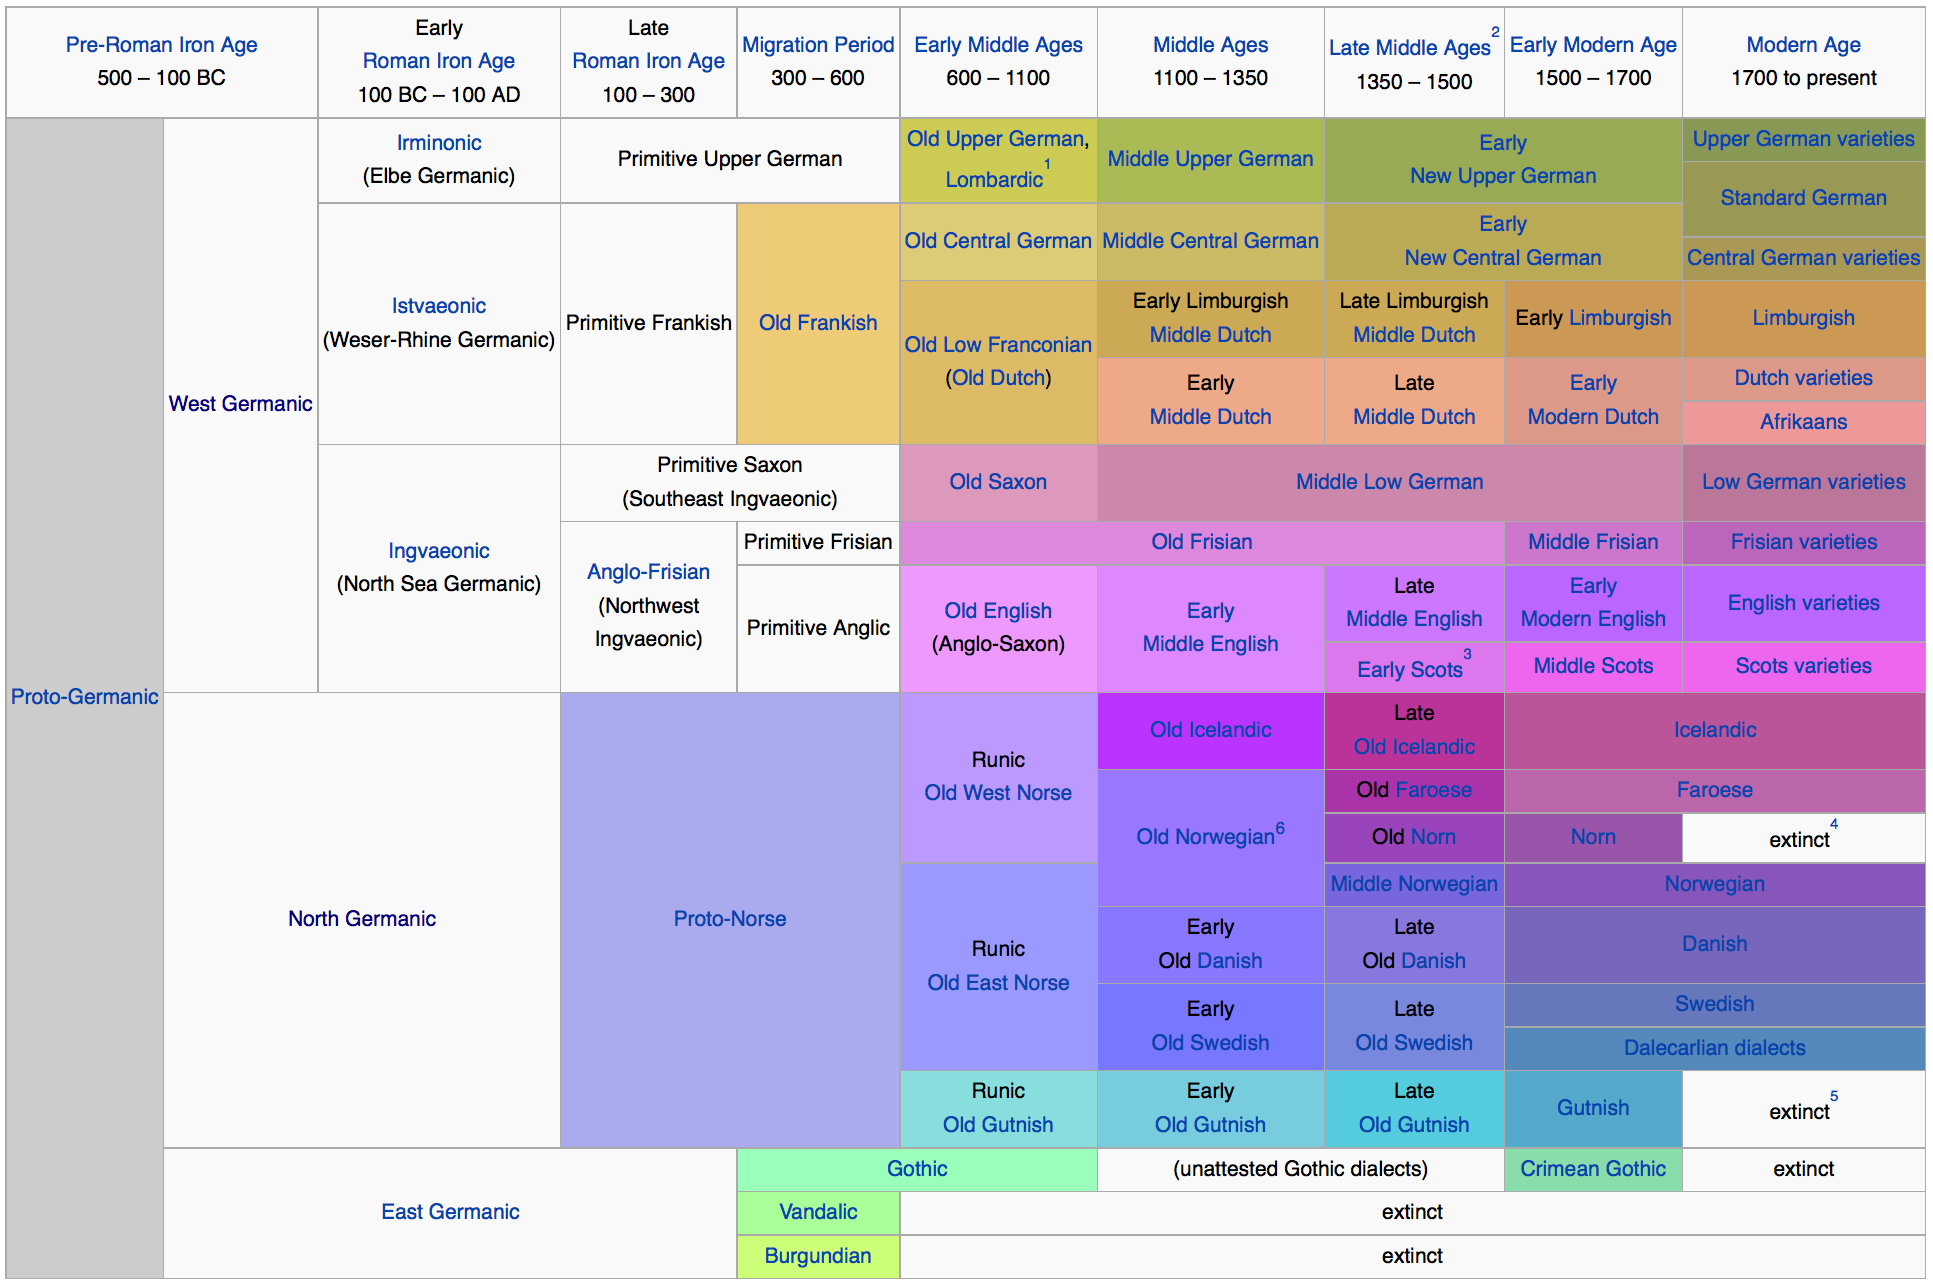
\includegraphics[width=.75\textwidth]{Bilder/germanic-wikipedia}

\oneline{Quelle: Englische Wikipedia: \url{https://en.wikipedia.org/wiki/Germanic_languages\#Diachronic}}


}



\subsection{Drei Zweige des Germanischen}

\frame{
\frametitle{Drei Zweige des Germanischen}

\begin{itemize}
\item Aufteilung des Protogermanischen in drei Zweige:\\
Ost-, West- und Nordgermanisch (etwa im ersten Jh.\ nach Chr.)
\pause

\item Ursachen:
\begin{itemize}
\item inhärente sprachliche Variation (Dialekte)
\item Migration (Sprachkontakt)
\item Standardisierung
\end{itemize}

\pause

\item Wir behandeln die Struktur germanischer Standardsprachen
\end{itemize}

}

\subsubsection{Ostgermanisch}

\frame{
\frametitle{Ostgermanisch}

\begin{itemize}
\item
ca.\ 100 v. Chr: Goten emigrieren von den dänischen Inseln
und aus Südschweden und treffen auf Vandalen und andere
Stämme
\pause
\item Sie konstituieren den ostgermanischen Zweig,\\ von dem nur
das Gotische überliefert ist
\pause
\item Mit dem Ende der Gotenreiche ist auch das Gotische
ausgestorben\\
(letzte Reste bis ca.\ 1800 auf der Halbinsel Krim)
\pause
\item Im 4.\ Jahrhundert übersetzte der westgotische Bischof
Wulfila die Bibel ins Gotische (Wulfila-Bibel)
\pause
\item  Bekannt ist vor allem das Manuskriptfragment in der
Universitätsbibliothek von Uppsala (Codex Argenteus)
\end{itemize}


}


\frame{
\frametitle{Wulfila-Bibel (Codex Argenteus)}

\begin{columns}[T]
\begin{column}{53mm}

\includegraphics[width=53mm]{Bilder/Wulfila_bibel}
\end{column}
\begin{column}{65mm}

Quelle: Wikipedia\\
\url{http://de.wikipedia.org/wiki/Bild:Wulfila_bibel.jpg}
\end{column}
\end{columns}

}

\subsubsection{Nordgermanisch}

\frame{
\frametitle{Nordgermanisch}

\begin{itemize}
\item erste Runen-Inschriften aus dem 6.\,Jh.
\item Sprache der Wikinger (800--1050) war noch relativ homogen
\item erst gegen Ende der Wikinger-Ära entstanden zwei Zweige:\\
 Ost-Skandinavisch (Altdänisch, Altschwedisch),\\
 West-Skandinavisch (Altnorwegisch, Altisländisch)
\end{itemize}

}



\subsubsubsection{Dänisch}

\frame{
\frametitle{Dänisch}

\begin{itemize}
\item Dänisch (dansk): offizielle Sprache des Königreichs Dänemark,
zweite Amtssprache der Färöer-Inseln und Grönlands (Inuit als
erste Sprache)
\item ca.\ 5,5 Millionen Sprecher*innen
\item ca.\ 50.000 Sprecher*innen in Schleswig Holstein
\item das Dänische hat sich von allen skandinavischen Sprachen am
weitesten von den gemeinskandinavischen Wurzeln entfernt
\end{itemize}

}



\subsubsubsection{Schwedisch}

\frame{
\frametitle{Schwedisch}

\begin{itemize}
\item Schwedisch (svenska):\\
offizielle Sprache in Schweden mit ca.\ 8,5 Millionen Muttersprachlern
\item erste Sprache von ca.\ 300.000 Sprecher*innenn in Finnland
\item Bis zur Wikingerzeit sind Dänisch und Schwedisch kaum
voneinander zu unterscheiden; 

ab ca.\ 800 entwickeln sie sich auseinander; 

seit ca.\ 1300 deutlich unterscheidbar
\end{itemize}

}


\subsubsubsection{Isländisch}

\frame{
\frametitle{Isländisch}

\begin{itemize}
\item Isländisch (íslenska) ist die westskandinavische Sprache Islands
seit der Besiedlung vor über 1000 Jahren
\item ca.\ 260.000 Sprecher*innen
\item kaum Variation (keine Dialekte)
\item Konservativ: von allen skandinavischen Sprachen hat das
Isländische die Flexion und seinen germanischen Erbwortschatz
am besten bewahrt.
\item Zunächst kaum Unterschiede zum Norwegischen,\\
dann auseinander entwickelt
\end{itemize}

}



\subsubsubsection{Norwegisch}


\frame{
\frametitle{Norwegisch}

\begin{itemize}
\item Norwegisch (norsk) kennt zwei Varietäten:\\
Dänisch-Norwegisch (bokmål) und Neu-Norwegisch (nynorsk). 

Beide sind offizielle Landessprachen und werden nebeneinander verwendet.
\item Insgesamt ca.\ 4,3 Millionen Sprecher*innen.
\item Von 1380--1814 war Dänisch die Schriftsprache;\\
gesprochen wurden lokale Dialekte
\item norwegischer Standard musste daher erst geschaffen werden;\\
Ivar Aasen (1813--1896): nynorsk; offiziell anerkannt 1885
\item bokmål (`Buchsprache') ist die erste Sprache der Mehrheit
\end{itemize}

}




\subsubsubsection{Färöisch}

\frame{
\frametitle{Färöisch}

\begin{itemize}
\item Färöisch oder Färingisch (føroyskt) ist, zusammen mit Dänisch,\\
die offizielle Sprache der Färöer-Inseln
\item 47.000 Sprecher*innen
\item Färöer-Inseln gehören seit 1816 zu Dänemark, \\
seit 1948 Status eines autonomen Landesteils
\item Färöisch ist stark vom Dänischen beeinflusst
\item Schriftsprachliche Überlieferung erst seit 1773 und auch dann nur spärlich\\
(dies im Gegensatz zum Isländischen)
\end{itemize}

}




\subsubsection{Westgermanisch}

\frame{
\frametitle{Westgermanisch}

\begin{itemize}
\item kein homogener Ursprung, sondern drei Zweige von
Dialektgruppen (Nordseegermanisch, Weser-Rheingermanisch,
Elbgermanisch)
\item aber keine 1-zu-1-Zuordnung dieser Dialektgruppen zu den
heutigen Standardsprachen
\end{itemize}

}




\subsubsubsection{Deutsch}

\author{Matthias Hüning, Stefan Müller}\institute[FU Berlin, Philosophie und Geisteswissenschaften]{}

\frame{
\frametitle{Deutsch}


\begin{itemize}
\item Deutsch ist offizielle Landessprache von 
\begin{itemize}
\item Deutschland (ca.\ 80 Millionen Sprecher*innen), 
\item Österreich (7,5 Millionen), 
\item Liechtenstein
(15.000), 
\item Schweiz (4,2 Millionen, von insgesamt 6,4 Millionen
Schweizern), 
\item Italien/Südtirol (270.000), 
\item Belgien (65.000),
\item Luxemburg (360.000).
\end{itemize}
\item In Luxemburg gilt neben dem nicht-ursprünglichen Deutsch auch
das ursprüngliche Lëtzebuergesch als offizielle Sprache.
\item Insgesamt hat das Deutsche ca.\ 97 Millionen Sprecher*innen, davon
ca.\ 90 Millionen Muttersprachler und 7 Millionen
Zweitsprachler (täglicher Gebrauch)
% = Migrationshintergrund
% Quelle Wikipedia 15.10.2013


\item ca.\ 80 Mio Fremdsprachler, davon ca. 55 Mio in der EU
\end{itemize}

}




\author{Matthias Hüning}\institute[FU Berlin, Philosophie und Geisteswissenschaften, Niederlandistik]{}


\frame{
\frametitle{Deutsch}

\begin{itemize}
\item Drei nationale Hauptvarianten (Deutschland, Österreich, Schweiz);\\
in anderen Staaten meist Minderheitensprache
\item Zwei Dialektgruppen: Niederdeutsch/Plattdeutsch und
Hochdeutsch
\end{itemize}

}



\subsubsubsection{Jiddisch}

\frame{
\frametitle{Jiddisch}

\begin{itemize}
\item Jiddisch ist eine von vielen jüdischen Sprachen.\\
heute von ca.\ 2 Millionen Menschen in verschiedenen Regionen der Welt gesprochen,\\
davon die meisten in den USA (1,25 Mill.)
\item Vor 100 Jahren lebten weit über 7 Millionen Sprecher*innen des
Jiddischen in Europa, die meisten in Russland und in Österreich-Ungarn.
\item Heute höchstens noch 75.000 Jiddisch-Sprachige in Westeuropa
\item Ursprung: mittelalterliches Deutsch, vermischt mit Hebräisch und
Aramäisch
\end{itemize}

}


\subsubsubsection{Pennsylvania German}

\frame{
\frametitle{Pennsylvania German}

\begin{itemize}
\item Pennsylvanisch (Deitsch, auch bekannt als Pennsylvanian Dutch)
hat ca.\ 300.000 Muttersprachler, vor allem in den USA
\item Sprachinseln, vor allem in Pennsylvania, Ohio und Indiana
\item Auswanderung im 17. und 18. Jahrhundert; Mitglieder
verschiedener protestantischer Glaubensrichtungen (Mennoniten,
Pietisten usw.)
\item Sprache baut hauptsächlich auf Pfälzer Dialekten auf
\item heute vor allem gesprochen von Amischen und Mennoniten
\end{itemize}

}



\subsubsubsection{Niederländisch}

\frame{
\frametitle{Niederländisch}

\begin{itemize}
\item Niederländisch (Nederlands) ist offizielle Landessprache in den Niederlanden\\
(ca.\ 15 Millionen Sprecher*innen),\\
eine der Landessprachen in Belgien (ca.\ 6 Millionen; knapp 4 Millionen
Wallonen).
\item Es ist die offizielle Verwaltungs- und Unterrichtssprache in Surinam\\
 (seit 1975 unabhängig) und auf Aruba und den niederländischen Antillen
\end{itemize}

}



\subsubsubsection{Afrikaans}

\frame{
\frametitle{Afrikaans}

\begin{itemize}
\item Afrikaans ist eine der offiziellen Sprachen Südafrikas\\
      (insgesamt über 10 Amtssprachen)
\item ca.\ 6,4 Millionen Muttersprachler,
davon 6,2 Millionen in Südafrika\\ (= ca.\ 15\,\% der Bevölkerung) und 150.000 in Namibia
\item seit Mitte des 17.\ Jh.; Entwicklung aus niederländischen Dialekten;\\
Afrikaans wird seit dem frühen 19.\ Jh. als
eigenständige Sprache gesehen
\item Sprachkontakt; heute starker Einfluss des Englischen
\item starke Tendenzen zu struktureller Vereinfachung im
Sprachsystem
\end{itemize}

}



\subsubsubsection{Friesisch}

\frame{
\frametitle{Friesisch}

Drei Varietäten, untereinander nicht verständlich:\begin{itemize}
\item Nordfriesisch, ca.\ 10.000 Sprecher*innen, vor allem auf den
nordfriesischen Inseln (Amrum, Sylt, Helgoland)
\item Ostfriesisch, in Ostfriesland ausgestorben.\\
Überbleibsel: das Saterfriesische (wird in der Gemeinde Saterland im Landkreis
Cloppenburg von etwa 1.000 bis 2.500 Menschen
gesprochen)
\item Westfriesisch, niederländische Provinz Friesland,\\
 ca.\ 350.000 Muttersprachler
\end{itemize}


}



\subsubsubsection{Englisch}

\frame{
\frametitle{Englisch}

\begin{itemize}
\item Englisch hat gegen Ende des 20.\ Jh. ca.\ 570 Millionen Sprecher*innen in
aller Welt (337 Mill. Muttersprachler, 235 Mill. Zweitsprachler)
\begin{itemize}
\item USA: 227 Mill. Muttersprachler; 
\item Großbritannien: 57 Mill.;
\item Nigeria: 43 Mill.; 
\item Kanada: 24 Mill.; 
\item Australien: 17 Mill.; 
\item Irland: 3,5 Mill.; 
\item Neuseeland: 3,2 Mill.
\end{itemize}
\item Viele nationale Varianten (vor allem Aussprache)
\item Geschätzte 1 bis 1,5 Milliarden Menschen besitzen aktive oder
passive Englischkenntnisse
\item Amtlicher Status in 59 Staaten
\item Weltweit wichtigste Wissenschaftssprache
\end{itemize}

\pause\pause\pause
}



%% -*- coding:utf-8 -*-
\frame{
\frametitle{Source code of the slides}

The source code of the slides is available on GitHub:

\url{https://github.com/stefan11/Germanic-Slides-English}

\medskip
The source code of the book as well:

\url{https://github.com/langsci/353}

}

%% -*- coding:utf-8 -*-
\author{Stefan Müller}\institute[HU Berlin, Institut für deutsche Sprache und Linguistik, Syntax]{}

\settowidth\jamwidth{(Niederländisch)}

\subtitle{Phenomena}

\section{Phenomena}

\huberlintitlepage[22pt]

\outline{

\begin{itemize}
%\item {Überblick über die germanischen Sprachen}
\item \alert{Phenomena}
\item Phrase structure grammars and \xbart
\item Valence, order of arguments and adjuncts
\item Verb clusters in SOV langauges
\item Verbposition: Verb first and verb second order
\item Passive
%\item embedded sentences
\end{itemize}

}



% \frame{
% \frametitle{Übungsaufgaben/Wiederholung}


% Bestimmen Sie in den folgenden Sätzen die topologischen Felder, die Wortarten der Wörter, die Kasus der Nominalgruppen und die
% grammatischen Funktionen und zeichnen Sie für einen Satz einen Strukturbaum in einem theoretischen
% Modell Ihrer Wahl (\zb Government \& Binding)!
% \eal
% \ex Der Mann lacht.
% \ex Der Frau hat der Mann das Buch gegeben, den wir kennen.
% \ex Ein Lied singend ging Peter voran.
% \ex Einen Aufsatz schreiben, der komplett neue Gedanken enthält,\\
%     können nur wenige.
% \zl

% }

\frame{
\frametitle{Introductory material}


Terminology (part of speech, grammatical functions, topological fields, \ldots): Chapter~1 in \citew{MuellerGT-Eng}.
\begin{refsection}

\nocite{MuellerGT-Eng}

\printbibliography[heading=none,notkeyword=this]

\end{refsection}

\pause

Overview of phenomena: Chapter~2 in \citew{MuellerGermanic}.


\begin{refsection}

\nocite{MuellerGermanic}

\printbibliography[heading=none,notkeyword=this]

\end{refsection}





}


  


\frame{
\frametitle{Variation}

\begin{itemize}
\item order:
\begin{itemize}
\item VO vs.\ OV
\item V2 vs. Non-V2
\item order of subjects and objects (fixed or free)
\item order of adverbs
\end{itemize}
\item verb clusters
\item subject requirement
\item passive
\begin{itemize}
\item personal passive
\item impersonal passive
\item objects of ditransitive verbs
\end{itemize}
\item expletives
\begin{itemize}
\item marking of clause type in main clauses (V2)
\item marking of clause type in embedded clauses (V3)
\end{itemize}
\end{itemize}


}


\subsection{Warning: OV/VO vs.\ V2/non-V2}

\frame{
\frametitle{Warning: OV/VO vs.\ V2/non-V2}


\begin{itemize}
\item Languages are classified according to order of subject, object and verb:
\begin{itemize}
\item SOV
\item SVO
\item \ldots
\end{itemize}
\item This does not mean that all sentences of a language always correspond to this pattern.
\item Languages are classified according to their type.

\item independent property: V2 or not V2.

\item third independent property:\\
      possibility to reorder subject and objects (Scrambling).

\item \citet{Haftka96a}:\\
      \emph{Deutsch ist eine V/2-Sprache mit Verbendstellung und freier Wortfolge}

German is a V2 language with verb in final position and free constituent order.

Sounds crazy, but it is not.

\end{itemize}
}


\subsection{Order of subject, object and verb}

\frame[shrink]{
\frametitle{Order of subject, object \& verb in the world's languages}

\medskip

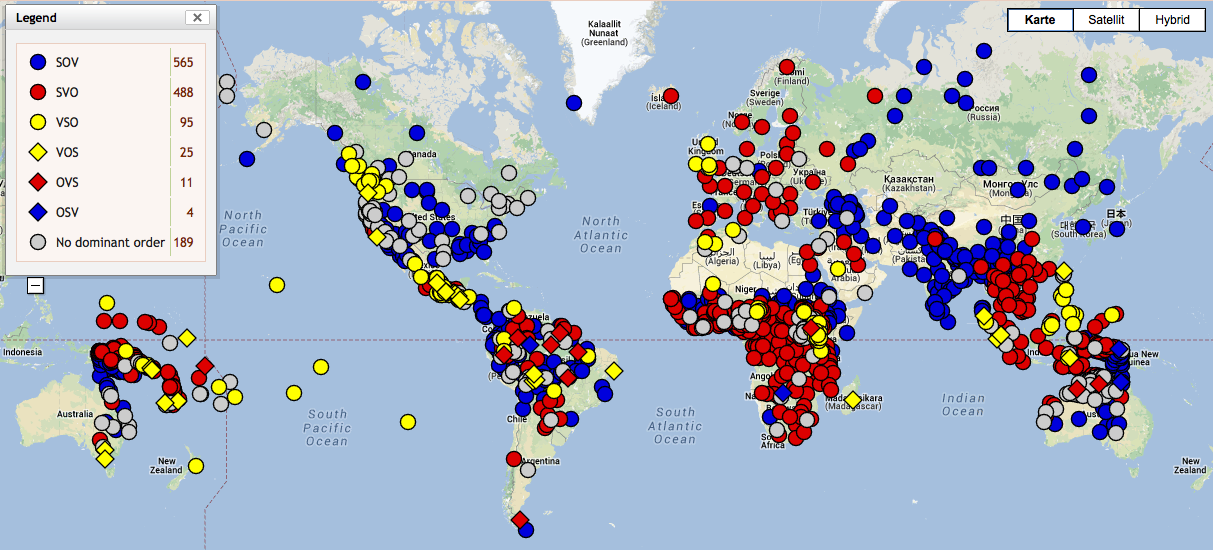
\includegraphics[width=\textwidth]{Bilder/WALS-SOV}

\vfill

{\small Matthew S. Dryer: Feature 81A: Order of Subject, Object and Verb,\\
 The World Atlas of Language Structures} 


}

\frame{
\frametitle{Subject, object and verb in the WALS}


\pause
\begin{itemize}
\item Subjects are arguments with more agent-like properties.
\pause
\item Objects are arguments with more patient-like properties.
\pause
\item This is not necessarily what we assume to be subjects and objects within traditional grammars
  of particular languages.\\ For example German: Subject = nominative \citep{Reis82}
\ea
\gll Der Aufsatz interessiert mich.\\
     the paper   interests    me\\
\glt `I am interested in the paper.'
\z
\end{itemize}



}

\frame{
\frametitle{Dryer: Word order}

\begin{itemize}
\item Dryer: Determining Dominant Word Order

\emph{Where a language is shown on one of the word order maps as having a particular order as the dominant
order in the language, this means that it is either \blaubf{the only order possible} or the order
that is \blaubf{more frequently used}.


I base my classification of Macushi here on the frequency counts, and since no order is more than
twice as frequent as the next most frequent order, I treat this language as lacking a dominant order
of subject, object, and verb.}

\bigskip

German, Dutch and Frisian are V2 languages, that is, SVO and SVAuxOV orders are the result of verb
fronting with a semantic function. These languages are usually counted among the SOV languages as well.

\end{itemize}



}

\frame{
\frametitle{Subject, object, verb in Europe}

\begin{columns}[T]
\begin{column}{90mm}
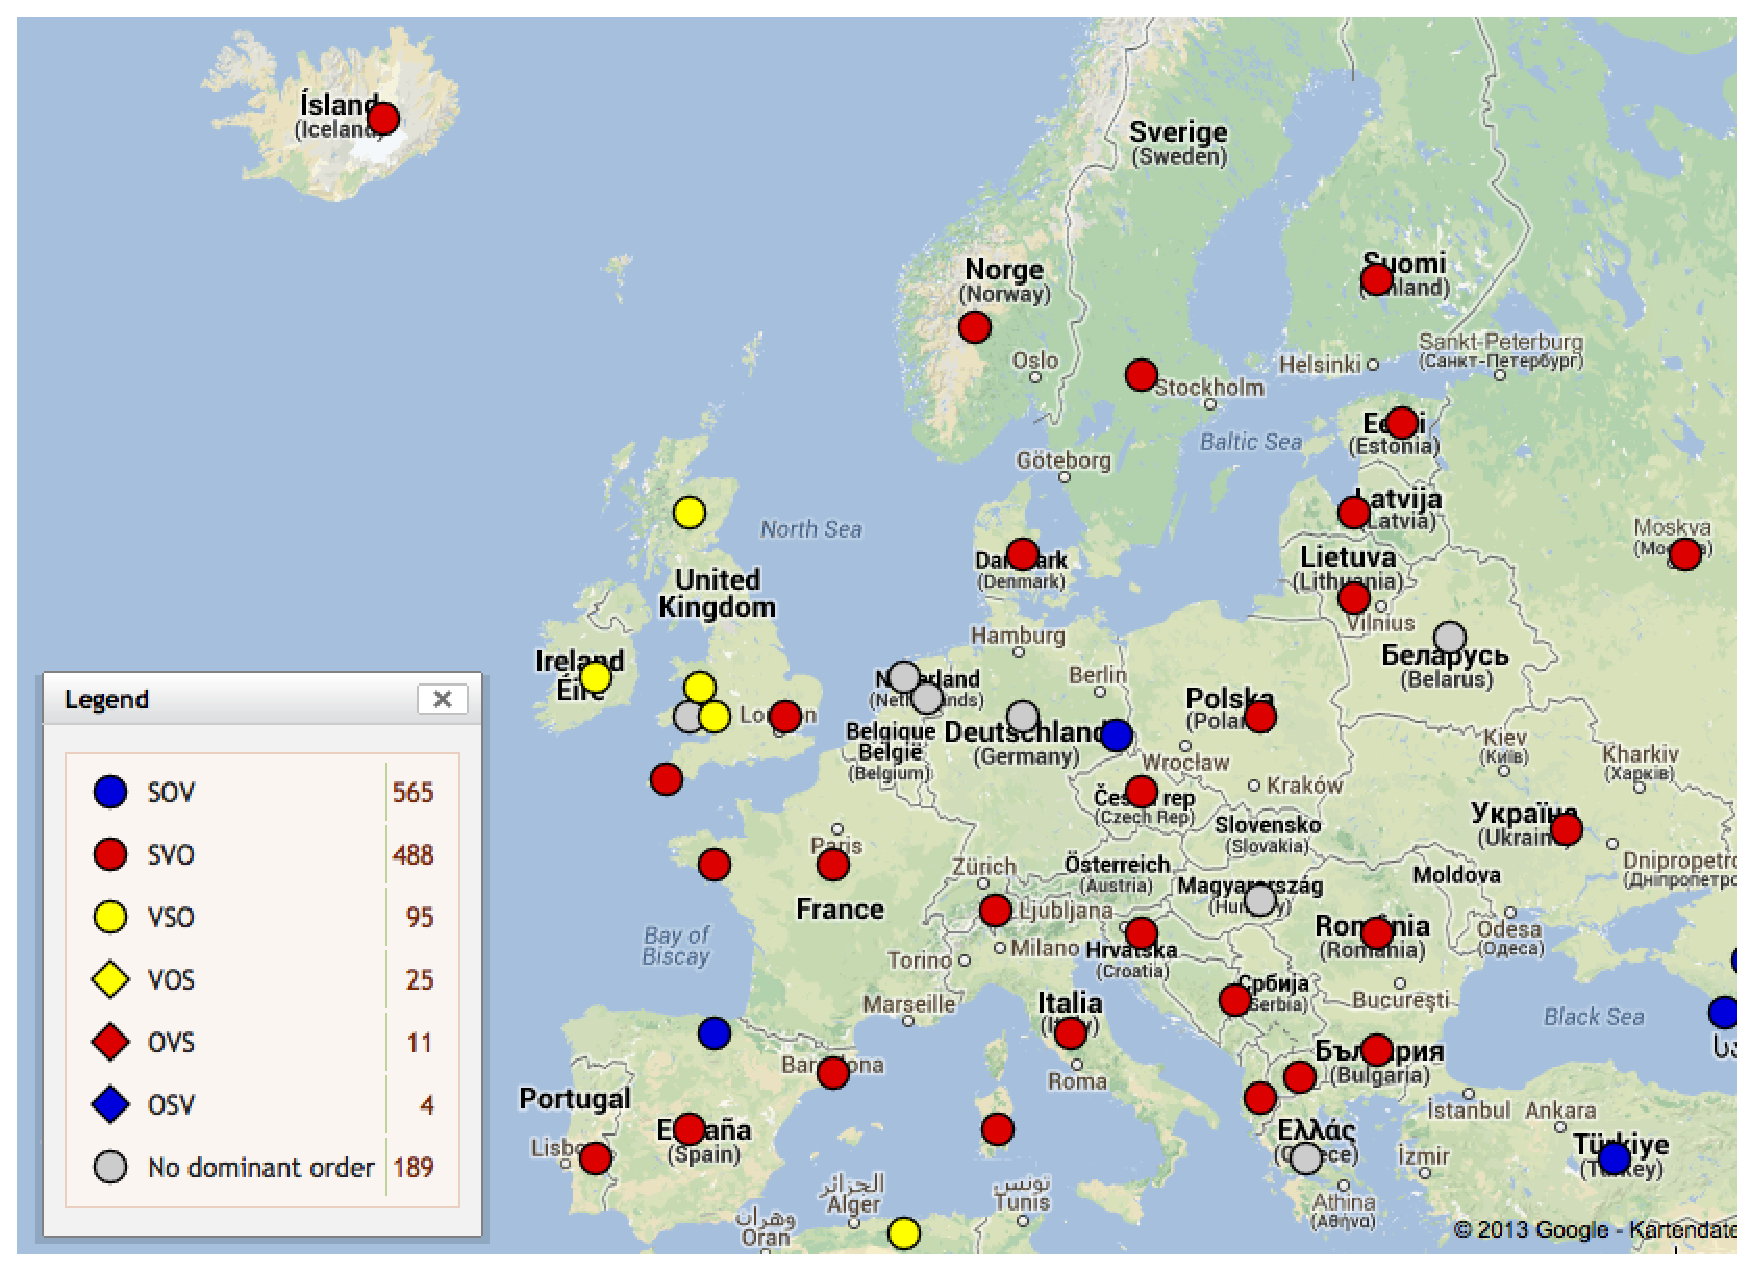
\includegraphics[width=\textwidth]{Bilder/WALS-SOV-Europa}
\end{column}
\begin{column}{25mm}
SVO:\\
Islandic,\\
Norwegian,\\
Swedish,\\
Danish,\\
English
\end{column}
\end{columns}
}


\frame{
\frametitlefit{Dryer: Feature 81b: Two Dominant Orders of Subject, Object, and Verb}

\begin{columns}[T]
\begin{column}{90mm}
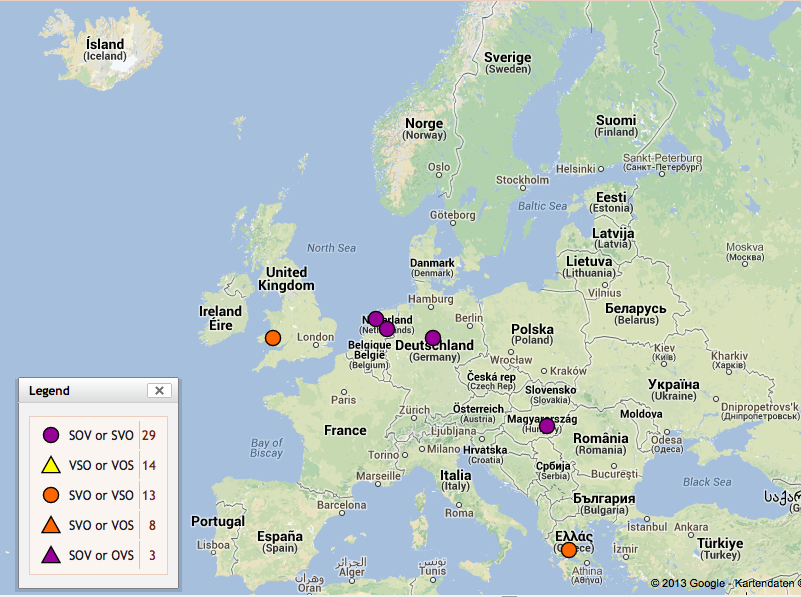
\includegraphics[width=.95\textwidth]{Bilder/WALS-SOV-Europa-no-dominant}
\end{column}
\begin{column}{30mm}
SVO oder SOV:\\
German,\\
Frisian,\\
Dutch
\end{column}
\end{columns}
% Walisisch: SVO oder VOS
% Friesisch
% Niederländisch
% Deutsch 
% Ungarisch

}
% Eisenberg89:409 zitiert Greenberg66 mit Deutsch als SVO.


\frame{
\frametitle{Languages without a dominant order in the WALS}

Dryer:

A third subtype of language lacking a dominant order consists of languages in which different word
orders occur but the choice is syntactically determined. For example, in \blaubf{German and Dutch}, the
dominant order is \blaubf{SVO in main clauses lacking an auxiliary} and \blaubf{SOV in subordinate clauses and
clauses containing an auxiliary} [\ldots]. Because this results in both orders being
common, neither order is considered dominant here and these two languages are shown on the map as
lacking a dominant word order. In general, if the word order varies according to whether there is an
auxiliary verb, the language is shown on the map as lacking a dominant order.


}

\frame{
\frametitle{Auxiliaries do not count, or do they?}

\eal
\ex 
\gll Kim sieht den Fuchs.\\
     Kim sees the fox\\
\glt `Kim sees the fox.'
\ex
\gll Kim hat den Fuchs gesehen.\\
     Kim has the fox seen\\
\glt `Kim has seen the fox.'
\zl
Dreyer classifies (\mex{0}a) as SVO and (\mex{0}b) as SAuxOV.\\
Aux is ignored so that the pattern counts as SOV.
\pause

}

\frame{
\frametitle{Other verb embedding verbs?}

But what about (\mex{1})?
\eal
\ex 
\gll Kim scheint den Fuchs zu sehen.\\
     Kim seems   the fox  to see\\ \hfill(SVOV?)
\glt `Kim seems to see the fox.'

\pause

\ex 
\gll Kim scheint den Fuchs gesehen zu haben.\\
     Kim seems   the fox  seen to have\\
\glt `Kim seems to have seen the fox.'
\zl

It is just the finite verb that is placed differently because of clause type marking.

}

\frame{
\frametitle{OV vs.\ VO: OV}

OV: Verbs follow the object:

\eal
\ex
\gll dass sie ihn sieht$_1$\\
     that she him sees\\\jambox{(German, SOV)}
\glt `that she sees him'
\ex
\gll dass sie ihn gesehen$_2$ hat$_1$\\
     that she him seen        has\\
\glt `that she has seen him'
\ex
\gll dass sie ihn gesehen$_3$ haben$_2$ muss$_1$\\
     that she him seen        have     must\\
\glt `that she must have seen him'
\zl

Embedding verbs follow embedded ones.

}

\frame{
\frametitle{OV vs.\ VO: VO}

VO: Verbs precede their object:

\eal
\ex
\gll at   hun ser$_1$ ham\\
     that she  sees    him\\\jambox{(\ili{Danish, SVO})}
\ex
\gll at   hun have$_1$ set$_2$ ham\\
     that she  has      seen    him\\
\ex
\gll at   hun må$_1$ have$_2$ set$_3$ ham\\
     that she  must   have     seen   him\\
\zl

OV: German, Dutch, Afrikaans, \ldots

VO: English, Danish, Norwegian, Swedish, \ldots

}

\frame{
\frametitle{Particle verbs and resultative constructions}

%[Section~15.2]
\citet{Haider2020a}: further differences between VO and OV languages:

Particle verbs:
\eal
\ex Kim will \alert{look up} the information.      \hfill(verb < particle)
\ex Kim wird die Information \alert{nachschlagen}. \hfill(particle < verb)
\zl
\pause

Resultative constructions:
\eal
\ex Kim will \alert{fish} the pond \alert{empty}.       \hfill(verb < pred)
\ex Kim wird den Teich \alert{leer} \alert{fischen}.    \hfill(pred < verb)
\zl

}

\subsection{V2}

\frame{
\frametitle{V2}

\begin{itemize}
\item German (and other Germanic languages) are V2 languages:\\
      The finite verb is in second position in assertions and \emph{w} questions.
\item An arbitrary constituent can be placed in front of it:
\eal
\ex 
\gll Das Kind  gibt dem Eichhörnchen jetzt eine Nuss.\\
     the child gives the squirrel now a nut\\\jambox{(\ili{German})}
\glt `The child gives the squirrel a nut now.'
\ex 
\gll Dem Eichhörnchen gibt das Kind jetzt eine Nuss.\\
     the squirrel gives the child now a nut\\
\ex 
\gll Eine Nuss gibt das Kind dem Eichhörnchen jetzt.\\
     a nut gives the child the squirrel now\\
\ex 
\gll Jetzt gibt das Kind dem Eichhörnchen eine Nuss.\\
     now gives the child the squirrel a nut\\
\zl
% \eal
% \ex 
% \gll Wer gibt dem Eichhörnchen jetzt eine Nuss?\\  
%      who gives the squirrel now a nut\\\jambox{(\ili{German})}
% \glt `Who gives the squirrel a nut now?'
% \ex 
% \gll Wem gibt das Kind jetzt eine Nuss?\\
%      who gives the child now a nut\\
% \glt `Who does the child give a nut to now?'
% \ex 
% \gll Was gibt das Kind dem Eichhörnchen jetzt?\\
%      what gives the child the squirrel now\\
% \glt `What does the child give the squirrel now?'
% \ex 
% \gll Wann gibt das Kind dem Eichhörnchen eine Nuss?\\
%      when gives the child the squirrel a nut\\
% \glt `When does the child give the squirrel a nut?'
% \zl
\end{itemize}

}

\frame{
\frametitle{V2 vs.\ non-V2}

\begin{itemize}
\item All Germanic languages are V2, except English:
\eal
\ex Bagels mag ich.\jambox{(German)}
\ex Bagels, I like.\jambox{(English)}
\zl 


\eal
\ex Gestern gab ich dem Eichhörnchen eine Nuss.\jambox{(German)}
\ex Yesterday, I gave the squirrel a nut.\jambox{(English)}
\zl 

\item There is fronting in English, but the fronted constituent is placed\\ before the subject and the
  verb.

\end{itemize}

}

\frame{
\frametitle{Non-extractable Elements}

Allmost all arguments can be frotned in V2 langauges.

Not all objects may be fronted in English (speaker dependent) \citep[\page 258]{Hudson92a-u}:

\eal
\judgewidth{\%}
\ex[]{
We give children sweets.
}
\ex[]{
These sweets, we give children \_.
}
\ex[\%]{
These children, we give \_ sweets.
}
\zl

}

\frame{
\frametitle{Fronting may cross clause boundaries}



\ea
\gll [Über dieses Thema]$_i$ habe ich sie gebeten, [[einen Vortrag \_$_i$~] zu halten].\footnotemark\\
     \spacebr{}about this topic  have I her asked \hphantom{[[}a talk {} to hold\\\german
\footnotetext{
Adapted from \citew[\page 21]{HN89b}.
}
\glt `I asked her to give a talk about this topic.'
\z

This means that V2 cannot be local reordering of constituents.


}


\frame{
\frametitle{V2 and OV/VO}

\begin{itemize}
\item V2 is independent of VO/OV. Danish is SVO and V2.
\eal
\ex 
\gll Gert har læst bogen.\\
     Gert has read book.\textsc{def}\\\danish
\ex
\gll Bogen har Gert læst.\\
     book.\textsc{def} has Gert read\\
\zl


\end{itemize}

}

\frame{
\frametitle{Englisch as Residual V2}

There is a residuum of V2 structures in questions:
\eal
\ex Which book did Sandy read?
\ex Which book did Sandy give to Kim?
\ex To whom did Sandy give the book?
\zl

\citet[\page 375]{Rizzi1990a-u}:  \emph{residual V2 language}


}


\frame{
\frametitle{Satztypen}

Satztypen werden über Verbstellung kodiert. Neben Aussagesätzen und \emph{w}-Fragesätzen gibt es
auch V2-Imperative:

\ea
Jetzt gib ihr das Buch!
\z
\pause

Ansonsten: Entscheidungsfragen und Imperative als V1:
\eal
\ex Gibt er ihr das Buch?
\ex Gib ihr das Buch!
\zl

} 


\frame{
\frametitle{V2 ist selten}

V2 ist selten \citep[\page 343]{Holmberg2015a}.

\begin{itemize}
\item germanische Sprachen (außer Englisch, \citealp{HP86a-ed})
\item modernes Bretonisch \citep{BK2000a-u}
\item Estnisch
\item Altfranzösisch \parencites[Section~1.3]{Adams1987a-u}[Section~2.1.2]{Roberts93a-u}[Chapter~2]{Vance97a-u},
  Altitalienisch, Altspanisch \citep[Section~3.3.2]{Fontana97a-u}, 
\item Rätoromanisch \citep{Poletto2002a-u,Anderson2006a-u},
\item das Kashmiri (Indien, Pakistan, \citealp[Chapter~4]{Bhatt99a-u})
\item Inguschisch (autonomen Republik Inguschetien, Russische Föderation)
\item die austronesischen Sprachen Taiof und Sisiqa, \citep[\page 495]{Ross2004a-u} % wieder aus der englischen Wikipedia verschwunden
\item die Sprache brasilianischer Ureinwohner*innen Karitiana aus der Tupí-Familie \citep{Storto2003a-u} 
% Ist vielleicht nur X2 sowas wie die australischen Sprachen (Bayer2010)
%\item die uto-aztekische Sprache Tohono O'odham\\
%      (Südwesten der USA sowie im Norden Mexikos).
\end{itemize}



}





\subsection{Scrambling}

\frame{
\frametitle{Scrambling oder nicht}

Germanische OV-Sprachen (Deutsch, \ldots):\\
prinzipiell alle Abfolgen von Argumenten möglich:
\eal
\ex {}[weil] \rot{das Kind} \gruen{dem Eichhörnchen} \blau{die Nuss} gibt
\ex {}[weil] \rot{das Kind} \blau{die Nuss} \gruen{dem Eichhörnchen} gibt
\ex {}[weil] \blau{die Nuss} \rot{das Kind} \gruen{dem Eichhörnchen} gibt
\ex {}[weil] \blau{die Nuss} \gruen{dem Eichhörnchen} \rot{das Kind} gibt
\ex {}[weil] \gruen{dem Eichhörnchen} \rot{das Kind} \blau{die Nuss} gibt
\ex {}[weil] \gruen{dem Eichhörnchen} \blau{die Nuss} \rot{das Kind} gibt
\zl

\pause

Germanische VO-Sprachen (Englisch, \ldots): Argumente haben eine feste Stellung.
\eal
\ex because \rot{the child} gives \gruen{the squirrel} \blau{the nut}
\ex because \rot{the child} gives \blau{the nut} \gruen{to the squirrel} 
\zl
\emph{Dative Shift} erfordert Umkategorisierung. Markierung durch Präposition.


}

\subsection{Stellung der Adverbialien}

\frame{
\frametitle{Stellung der Adverbialien}


Deutsch, Niederländisch, \ldots: Stellung der Adverbien frei:
\eal
\ex weil das Kind dem Eichhörnchen die Nuss \blauit{gestern} gab
\ex weil das Kind dem Eichhörnchen \blauit{gestern} die Nuss gab
\ex weil das Kind \blauit{gestern} dem Eichhörnchen die Nuss gab
\ex weil \blauit{gestern} das Kind dem Eichhörnchen die Nuss gab
\zl

\pause

Dänisch, Englisch, \ldots: Adverbien stehen vor oder nach der VP:
\eal
\ex because the child \blauit{often} [\gruen{gave the squirrel the nut}]
\ex because the child [\gruen{gave the squirrel the nut}] \blauit{often}
\zl

\pause
Extremfall verschachtelte VPen \citep[§ 8.20, 495]{QGLS85a-u}:
\ea
It [\blauit{certainly} [\sub{VP} may [\blauit{possibly} [\sub{VP} have [\blauit{indeed} [\sub{VP} been\\ {}[\blauit{badly} [\sub{VP} formulated]]]]]]]].
\z

}

\if0

\subsection{Eingebettete Sätze}

\subsubsection{Konjunktional eingeleitete Nebensätze}

\frame{
\frametitle{Deutsch: eingebettete Sätze sind VL}

\begin{itemize}
\item Deutsch, Niederländisch, \ldots: V-letzt:

\ea
Ich weiß, dass Aicke das Buch heute gelesen hat.
\z

\pause
Stellung der anderen Konstituenten ist frei:
\eal
\ex Ich weiß, dass das Buch Aicke heute gelesen hat.
\ex Ich weiß, dass das Buch heute Aicke gelesen hat.
\zl

\end{itemize}

}

\frame{
\frametitle{Englisch: eingebettete Sätze SVO}


\begin{itemize}
\item Englisch: eingebettete Sätze SVO
\ea[]{
I  know that Kim has read the book yesterday.
}
\z

%% \pause
%% Andere Stellungen sind nicht möglich:
%% \eal
%% \ex[*]{
%% I know that has Max read the book yesterday.
%% }
%% \ex[*]{
%% I know that yesterday Max has read the book.
%% }
%% \zl

\end{itemize}

}



\frame{
\frametitle{Dänisch: eingebettete Sätze SVO oder V2}


\begin{itemize}
\item Dänisch: eingebettete Sätze SVO oder V2
\ea[]{
\gll Jeg  ved, at   Gert ikke  har læst  bogen          {i dag}.\\
     ich weiß dass Gert nicht hat gelesen Buch.{\sc def} heute\\\jambox{(SVO)}
}
\z
Negation hilft, Verbstellung zu bestimmen:
\ea[]{
\gll Jeg  ved, at   Gert har ikke  læst  bogen          {i dag}.\\
     ich weiß dass Gert hat nicht gelesen Buch.{\sc def} heute\\\jambox{(V2)}
}
\z



\pause
Andere Konstituenten in Initial-Stellungen sind möglich, \dash klares V2:
\eal
\ex[]{
\gll Jeg  ved, at   {i dag} har Gert ikke læst bogen.\\
     ich weiß dass heute   hat Gert nicht gelesen Buch.{\sc def}\\
}
\ex[]{
\gll Jeg ved, at   bogen          har Gert ikke  læst {i dag}.\\
     ich weiß dass Buch.{\sc def} hat Gert nicht gelesen heute\\
}
\zl

%% \ex[*]{
%% \gll Jeg  ved, at   {i dag} Gert har læst bogen.\\
%%      ich weiß dass heute   Gert hat gelesen Buch.{\sc def}\\
%% }
%%
%% \ex[*]{
%% \gll Jeg  ved, at   bogen          Gert har læst {i dag}.\\
%%      ich weiß dass Buch.{\sc def} Gert hat gelesen heute\\
%% }
%% \zl

\end{itemize}

}


\frame{
\frametitle{Jiddisch, Isländisch: eingebettete Sätze sind V2}

% Isländisch: Wikipedia (en)

\begin{itemize}
\item Jiddish: eingebettete Sätze sind V2 \citep[]{Diesing90a}:
\eal
\ex
\gll Ikh meyn  az   haynt hot Max geleyent dos bukh.\footnotemark\\
     ich   denke dass heute hat Max gelesen   das Buch\\
\footnotetext{\citew[\page 58]{Diesing90a}.}
\glt `Ich denke, dass Max heute das Buch gelesen hat.'

\ex% check!
\gll Ikh meyn  az   dos bukh hot Max geleyent.\\
     ich denke dass das Buch hat Max gelesen\\

\zl

\pause
Isländisch:
\ea 
\gll Engum         datt í hug,  að   vert  væri að reyna til     að kynnast honum.\footnotemark\\
     niemand.\DAT{} kam in Gedanke dass wert war  zu versuchen  \PREP{} zu kennen ihn\\\icelandic
\footnotetext{\citew[\page 75]{Maling90a-u}.}
\glt `Niemand kam der Gedanke, dass es sich lohnen könnte zu versuchen, ihn kennenzulernen.'
\z



\end{itemize}

}


\subsubsection{Interrogativnebensätze}


\frame{
\frametitle{Deutsch: Interrogativnebensätze \emph{w} + VL}

\begin{itemize}
\item Deutsch, Niederländisch, \ldots: \emph{w} + V-letzt:

\eal
\ex Ich weiß, wer heute das Buch gelesen hat.
\ex Ich weiß, was Aicke heute gelesen hat.
\zl

Interrogativnebensätze beginnen mit einer \emph{w}-Phrase.

\pause
\item Die \emph{w}-Phrase kann von weit her kommen:
\ea
Ich weiß nicht, [\gruen{über welches Thema}]$_i$ sie versprochen hat,\\
{}[[einen Vortrag \_$_i$] zu halten].
\z

\pause
\item Stellung der anderen Konstituenten ist frei:
\eal
\ex Ich weiß, was keiner diesem Eichhörnchen geben würde.
\ex Ich weiß, was diesem Eichhörnchen keiner geben würde.
\zl



\end{itemize}

}

\frame{

\frametitle{Dänisch, Englisch: Interrogativnebensätze  \emph{w} + SVO}


\begin{itemize}
\item Dänisch: Interrogativnebensätze sind \emph{w} + SVO

\eal
\ex
\gll Jeg ved, hvad Gert har givet ham.\\
     ich weiß was Gert  hat gegeben ihm\\
\glt `Ich weiß, was Gert ihm gegeben hat.'
\ex
\gll Jeg ved, hvem Gert har givet   bogen.\\
     ich weiß wem  Gert hat gegeben Buch.{\sc def}\\
\glt `Ich weiß, wem Gert das Buch gegeben hat.'
\zl

\end{itemize}

}

\frame{
\frametitle{Jiddish: Interrogativnebensätze \emph{w} + V2}

\begin{itemize}
\item Jiddish: Interrogativnebensätze \emph{w} + V2 \citep[Abschnitte~4.1, 4.2]{Diesing90a}

%% \ea
%% %\ex
%% \label{vosmaks}
%% \gll Ikh veys nit   [vos Max hot gegesn].\footnotemark\\
%%      ich weiß nicht \hspaceThis{[}was Max hat gegessen\\
%% \footnotetext{\citew[S.\,68]{Diesing90a}.}
%% \glt `Ich weiß nicht, was Max gegessen hat.'

%% %% \ex%check
%% %% \gll Ikh veys nit   [vos              hot Max gegesn].\footnotemark\\
%% %%      ich weiß nicht \hspaceThis{[}was heute hat Max gegessen\\
%% %% \footnotetext{\citew[S.\,68]{Diesing90a}.}
%% %% \glt `Ich weiß nicht, was Max heute gegessen hat.'


\ea
\gll Ir veyst efsher [avu            do    voynt Roznblat   der goldshmid]?\footnotemark\\
     Sie wissen vielleicht  \spacebr{}wo da wohnt Roznblat der Goldschmied\\
\glt `Wissen Sie vielleicht, wo Roznblat der Goldschmied wohnt?' 
\footnotetext{
\citew[S.\,65]{Diesing90a}. Zitiert aus Olsvanger, \emph{Royte Pomerantsn}, 1949
}
\z
\end{itemize}

}



\subsection{Expletiva zur Satztypmarkierung}

\frame{
\frametitle{Expletiva zur Satztypmarkierung}

\begin{itemize}
\item Germanische Sprachen benutzen Expletiva, um Satztypen kenntlich zu machen,
      falls keine andere Konstituente die entsprechende Position füllt.
\pause
\item Deutsch V2-Hauptsätze

\eal
\ex Drei Reiter ritten zum Tor hinaus.
\ex \rot{Es} ritten drei Reiter zum Tor hinaus.
\zl
\end{itemize}


}

\frame{
\frametitle{Dänisch: \emph{w}-Sätze mit extrahiertem Subjekt}

\begin{itemize}
\item Dänisch: \emph{w} + SVO\\
      Bei Subjektextraktion muss Extraktion explizit kenntlich gemacht werden:
\eal
\ex[]{
\gll Politiet ved ikke, \gruen{hvem} \rot{der}   havde placeret bomben.\\
     Polizei.{\sc def} weiß nicht wer {\sc expl} hat plaziert Bombe.{\sc def}\\
\glt `Die Polizei weiß nicht, wer eigentlich die Bombe plaziert hat.'
}
\ex[*]{
\gll Politiet ved ikke, \gruen{hvem} havde placeret bomben.\\
     Polizei.{\sc def} weiß nicht wer hat plaziert Bombe.{\sc def}\\
}
\zl

\pause

Expletivum macht Extraktion sichtbar:
\eal
\ex[*]{ 
\gll [\gruen{hvem}$_i$     [\trace$_i$ havde placeret bomben]]\\
     \spacebr{}wer {}          hat   plaziert Bombe.\textsc{def}\\\danish
}
\ex[]{
\gll [\gruen{hvem}$_i$     [\rot{der}                    havde \trace$_i$ placeret bomben]]\\
     \spacebr{}who \spacebr{}\textsc{expl} hat   {}         plaziert Bombe.\textsc{def}\\
}
\zl


\end{itemize}

}

\frame{
\frametitle{Jiddish: \emph{w}-Sätze mit extrahiertem Subjekt}

\begin{itemize}
\item Jiddish: Interrogativnebensätze \emph{w} + V2\\
%% \ea
%% \label{vosmaks}
%% \gll Ikh veys nit   [vos Max hot gegesn].\footnotemark\\
%%      ich weiß nicht \hspaceThis{[}was Max hat gegessen\\
%% \footnotetext{\citew[S.\,68]{Diesing90a}.}
%% \glt `Ich weiß nicht, was Max gegessen hat.'
%% \z
%% \pause
%% \item 
  Wenn %das Subjekt extrahiert wird und 
kein anderes Element ins Vorfeld soll, muss dort ein \emph{es} stehen:

\eal
\ex[]{
\gll ikh hob  zi  gefregt \gruen{ver} \rot{es}         iz beser  far ir\\
     ich habe sie gefragt wer         {\sc expl} ist besser für sie\\
\glt `Ich habe sie gefragt, wer besser für sie ist.'}
\ex[]{
\gll ikh hob  im  gefregt \gruen{vemen} \rot{es}        kenen ale dayne khaverim\\
     ich habe ihn gefragt wen           {\sc expl} kennen alle deine Freunde\\
\glt `Ich habe ihn gefragt, wen alle deine Freunde kennen.}
\zl

\end{itemize}

}

\fi

\subsection{Verbalkomplexbildung}


\frame{
\frametitle{Verbalkomplexbildung nur in OV-Sprachen}

\begin{itemize}
\item Normalerweise stehen Objekte neben ihren Verben:
\ea
Somebody promised him [to read a book].
\z
\ea
weil    jemand   [ihr [das Buch zu lesen] versprochen] hat\\
\z

\pause

\item Deutsch, Niederländisch erlauben Verbalkomplexbildung:
\ea
weil \highlight{es}<2> \highlight{ihr}<3> \highlight{jemand}<4> \highlight{zu lesen}<2> \highlight{versprochen}<3> \highlight{hat}<4>. \citep{Haider90b}
\z

\pause
\pause
\pause
Die Verben am Ende verhalten sich wie ein einfaches Verb $\to$\\
Umordnung der Argumente ist möglich.


\pause
\item Englisch, Dänisch, \ldots{} erlauben keine Umordnung von Konstituenten

\eal
\judgewidth{\#}
\ex[*]{
Somebody promised a book her to read.
}
\ex[\#]{
Somebody promised to read her a book.
}
\zl

\end{itemize}


}

\subsection{Obligatorische Subjekte}

\frame{
\frametitle{Obligatorische Subjekte}

\begin{itemize}
\item Englisch, Dänisch brauchen ein Subjekt

\pause
\item Deutsch kommt ohne Subjekt klar:
\eal
\ex Ihm graut vor der Prüfung.
\ex Heute wird nicht gearbeitet.
\zl

\pause
\item Oft kann bei subjektlosen Verben ein expletives Subjekt angeschlossen werden:
\ea
Ihm graut es vor der Prüfung.
\z
\pause
\item Aber manchmal geht auch das nicht:
\eal
\ex[]{
Mir ist schlecht.
}
\ex[*]{
Mir ist es schlecht.
}
\ex[*]{
weil es mir schlecht ist
}
\zl
%% Das geht mit "etwas" oder "viel" aber das sind wohl adverbiale Akkusative, sie können nicht durch
%% Pronomina ersetzt werden.
%% \eal
%% \ex[]{
%% Mir liegt an dir.
%% }
%% \ex[*]{
%% Mir liegt es an dir.
%% }
%% \zl

\end{itemize}

}


\subsection{Kasus}

\frame{
\frametitle{Kasus}

\begin{itemize}
\item Isländisch hat das am besten erhaltene Flexionssystem.
\pause
\item Im Vergleich zu anderen germanischen Sprachen ist Isländisch interessant,\\
      weil es Subjekte hat, die nicht im Nominativ stehen \citep{ZMT85a}.
\pause
\item Einheitliche Behandlung der Kasuszuweisung ist möglich:\\
\citew*{YMJ87}.

\end{itemize}


}

\subsection{Unpersönliches Passiv}

\frame[shrink]{
\frametitle{Unpersönliches Passiv}

\begin{itemize}
\item Das Deutsche erlaubt ein unpersönliches Passiv:
\ea[]{
\label{ex-gearbeitet-wurde}
weil noch gearbeitet wird
}
\z

\pause
\item Das Englische lässt kein unpersönliches Passiv zu.
\ea[*]{
because (it) was worked
}
\z

\pause
\item Dänisch schon, trotz Subjektbedingung: Expletivum wird eingefügt.
\eal
\label{ex-bliver-arbejder}
\ex 
\gll fordi der bliver arbejdet\\
     weil {\sc expl} wird gearbeitet\\
\glt `weil gearbeitet wird'
\ex
\gll fordi   der arbejdes\\
     weil  {\sc expl} arbeiten.{\sc pass}\\
\glt `weil gearbeitet wird'
\zl
\pause
\item Das Deutsche erlaubt kein Expletivum.

\end{itemize}
\pause\pause\pause

}


%      <!-- Local IspellDict: en_US-w_accents -->

%% -*- coding:utf-8 -*-

\subtitle{Phrase structure grammar and \xbar Theory}

\section{Phrase structure grammar and \xbar Theory}


\huberlintitlepage[22pt]


\outline{

\begin{itemize}
\item {Überblick über die germanischen Sprachen}
\item Phänomene
\item \alert{Phrasenstrukturgrammatiken und \xbart}
\item Valenz, Argumentanordnung und Adjunkte
\item Verbalkomplexbildung in den SOV-Sprachen
\item Verbstellung: Verberst- und Verbzweitstellung
\item Passiv
\item Eingebettete Sätze
\end{itemize}

}


\frame{
\frametitle{Literature}

The following is based on \citew[Kapitel~3]{MuellerGermanic}.


\begin{refsection}

\nocite{MuellerGermanic}

\printbibliography[heading=none,notkeyword=this]

\end{refsection}


}

\subsection{Phrase structure grammar}


\subsubsection{Phrase structure}

\frame{
\frametitle{Phrase structure}

\smallframe
\hfill%
\begin{tabular}{@{}l@{\hspace{1cm}}l@{}}
\scalebox{.7}{%
\begin{forest}
sm edges
[S
  [NP [Aicke;Aicke] ]
  [NP
    [Det [dem;the] ]
    [N [Affen;monkey] ] 
  ]
  [NP
    [Det [den;the] ]
    [N [Stock;stick] ] 
  ]
  [V [gibt;gives] ]
]
\end{forest}} &
\scalebox{.7}{%
\begin{forest}
sm edges
[V
  [NP [Aicke;Aicke] ]
  [V
    [NP
      [Det [dem;the] ]
      [N [Affen;monkey] ] ]
    [V
      [NP
        [Det [den;the] ]
        [N [Stock;stick] ] ]
      [V [gibt;gives] ] ] ] ]
\end{forest}}
\\
\\[-0.4ex]
\begin{tabular}{@{~}l@{ }l@{}}
NP & $\to$ Det, N            \\
S  & $\to$ NP, NP, NP, V  \\
\end{tabular} & \begin{tabular}{@{~}l@{ }l@{}}
NP & $\to$ Det, N  \\
V  & $\to$ NP, V\\
\end{tabular}\\
\end{tabular}
\hfill\mbox{}

\medskip
Rewrite rules are the real thing! Trees are just visualizations.\\
%
\pause%
%
Sometimes a bracket notation is used:\\
{}[\sub{S} [\sub{NP} Aicke] [\sub{NP} [\sub{Det} dem] [\sub{N} Affen]]  [\sub{NP} [\sub{Det} den] [\sub{N} Stock]] [\sub{V} gibt]]

\handoutspace
}

\iftoggle{psgbegriffe}{
\subsubsection{Terminology}


\frame{
\frametitle{Nnode}

\vfill
\psset{xunit=5mm,yunit=5mm,nodesep=8pt}
\hfill
\begin{pspicture}(0,0)(14,7.4)
\rput(3,7){\rnode{xp}{A}}
\rput(1,4){\rnode{up}{B}}\rput(5,4){\rnode{xs1}{C}}
\rput(5,1){\rnode{vp}{D}}

\psset{angleA=-90,angleB=90,arm=0pt}
\ncdiag{xp}{up}\ncdiag{xp}{xs1}%
\ncdiag{xs1}{vp}\ncdiag{xs1}{xs2}%
\ncdiag{xs2}{wp}\ncdiag{xs2}{x}%
\ncdiag{wp}{yp}\ncdiag{wp}{ws}%

\pause

%\mode<beamer>{
\psset{linecolor=red}%radius=1em}
%}
%\pscircle(3,7){2ex}
\cnode[linewidth=1.5pt](3,7){1.7ex}{nodeA}
\pscircle[linewidth=1.5pt](1,4){1.7ex}\cnode[linewidth=1.5pt](5,4){1.7ex}{nodeC}
\cnode[linewidth=1.5pt](5,1){1.7ex}{nodeD}

\pause

\rput[l](8,7){\rnode{verz}{verzweigend}}
\rput[l](8,6){\rnode{nverz}{n}icht verzweigend}

%\psset{angleA=180,angleB=0,arm=0pt,arrows=->}
\only<3>{
\ncline{->}{verz}{nodeA}
}
\pause
\only<4>{
\ncline{->}{nverz}{nodeC}
}
%\psgrid
\end{pspicture}
\hfill\hfill\mbox{}
\vfill
}

\frame{

\frametitle{Mother, daughter and sister}

\vfill
\psset{xunit=5mm,yunit=5mm,nodesep=8pt}
\hspace{1cm}%
%\begin{tabular}{@{}l@{\hspace{1cm}}l@{}}
\begin{pspicture}(0,0)(7.4,7.4)
\rput(3,7){\rnode{xp}{A}}
\rput(1,4){\rnode{up}{B}}\rput(5,4){\rnode{xs1}{C}}
\rput(5,1){\rnode{vp}{D}}

\psset{angleA=-90,angleB=90,arm=0pt}
\ncdiag{xp}{up}\ncdiag{xp}{xs1}%
\ncdiag{xs1}{vp}\ncdiag{xs1}{xs2}%
\ncdiag{xs2}{wp}\ncdiag{xs2}{x}%
\ncdiag{wp}{yp}\ncdiag{wp}{ws}%

%\psgrid
\end{pspicture}
\hspace{1cm}\raisebox{3cm}{\begin{tabular}[t]{@{}l@{}}
A is the mother of B and C\\
C is the mother of D\\
B is the sister of C\\
\end{tabular}}


As in genealogies

\vfill

}

\iftoggle{einfsprachwiss-exclude}{
\frame{
\frametitle{Dominance}

\vfill
\psset{xunit=5mm,yunit=5mm,nodesep=8pt}
\hspace{1cm}
\begin{pspicture}(0,0)(7.4,7.4)
\rput(3,7){\rnode{xp}{A}}
\rput(1,4){\rnode{up}{B}}\rput(5,4){\rnode{xs1}{C}}
\rput(5,1){\rnode{vp}{D}}

\psset{angleA=-90,angleB=90,arm=0pt}
\ncdiag{xs1}{xs2}%
\ncdiag{xs2}{wp}\ncdiag{xs2}{x}%
\ncdiag{wp}{yp}\ncdiag{wp}{ws}%

\alt<2>{
\mode<beamer>{
\psset{linecolor=red}
}
\ncdiag{->}{xp}{up}\ncdiag{->}{xp}{xs1}
}{
\ncdiag{xp}{up}\ncdiag{xp}{xs1}%
}
\alt<2,4>{
\mode<beamer>{
\psset{linecolor=red}
}
\ncdiag{->}{xs1}{vp}
}{
\ncdiag{xs1}{vp}
}
%\psgrid
\end{pspicture}
\hspace{1cm}\raisebox{3cm}{\begin{tabular}[t]{@{}l@{}}
A dominates \only<2->{B, C and D}\\
\only<3->{C dominates} \only<4->{D} \\
\end{tabular}}

\bigskip

A dominates B iff A is higher in the tree and\\
if there is a connection from A to B that goes downwards only.

\pause\pause\pause

\vfill

}

\frame{

\frametitle{Immediate dominance}

\psset{xunit=5mm,yunit=5mm,nodesep=8pt}
\hspace{1cm}
\begin{pspicture}(0,0)(7.4,7.4)
\rput(3,7){\rnode{A}{A}}
\rput(1,4){\rnode{B}{B}}\rput(5,4){\rnode{C}{C}}
\rput(5,1){\rnode{D}{D}}

\psset{angleA=-90,angleB=90,arm=0pt}
\ncdiag{C}{xs2}%
\ncdiag{xs2}{wp}\ncdiag{xs2}{x}%
\ncdiag{wp}{yp}\ncdiag{wp}{ws}%

\alt<2>{
\mode<beamer>{
\psset{linecolor=red}
}
\ncdiag{->}{A}{B}\ncdiag{->}{A}{C}
}{
\ncdiag{A}{B}\ncdiag{A}{C}%
}
\alt<4>{
\mode<beamer>{
\psset{linecolor=red}
}
\ncdiag{->}{C}{D}
}{
\psset{linecolor=black}
\ncdiag{C}{D}
}
%\psgrid
\end{pspicture}
\hspace{1cm}\raisebox{3cm}{\begin{tabular}[t]{@{}l@{}}
A dominates immediately \only<2->{B and C}\\
\only<3->{C dominates immediately} \only<4->{D} \\
\end{tabular}}

\bigskip

A dominates B immediately iff \\
A dominates B and there is no node C between A and B.

\pause\pause\pause


}


\frame{
\frametitle{Precedence}

\begin{description}[<+->]
\item[Precedence]~\\ A preceeds B iff A is to the left of B in the tree and\\
     none of the two nodes dominates the other.
\item[Immediate precedence]~\\ There is no element C between A and B.
\end{description}

}
}%\end{einfsprachwiss-exclude}
}%psgbegriffe


\subsubsection{A sample grammar}


\frame[shrink=8]{
\frametitle{Example derivation with a flat structure}

\vfill

\bigskip
\parskip0pt
\begin{tabular}[t]{@{}l@{ }l}
\highlight{NP}<5,8> & \highlight{$\to$ Det N}<5,8>\\          
\highlight{S}<10>  & \highlight{$\to$ NP NP NP V}<10>
\end{tabular}\hspace{2cm}%
\begin{tabular}[t]{@{}l@{ }l}
\highlight{NP}<2> & \highlight{$\to$ Aicke}<2>\\
\highlight{Det}<3>  & \highlight{$\to$ dem}<3>\\
\highlight{Det}<6>  & \highlight{$\to$ den}<6>\\
\end{tabular}\hspace{8mm}
\begin{tabular}[t]{@{}l@{ }l}
\highlight{N}<4> & \highlight{$\to$ Affen}<4>\\
\highlight{N}<7> & \highlight{$\to$ Stock}<7>\\
\highlight{V}<9> & \highlight{$\to$ gibt}<9>\\
\end{tabular}
\vfill

\begin{tabular}{@{}llllll@{\hspace{2.5cm}}l}
Aicke            & dem          & Affen          & den          & Stock & gibt                \pause\\
\highlight{NP}<2> & dem          & Affen          & den          & Stock & gibt & \only<handout>{NP $\to$ Aicke}  \pause\\
NP            & \highlight{Det}<3> & Affen          & den          & Stock & gibt & \only<handout>{Det $\to$ das}  \pause\\
NP            & Det            & \highlight{N}<4>  & den          & Stock & gibt & \only<handout>{N $\to$ Buch} \pause\\
NP            &              & \highlight{NP}<5> & den          & Stock & gibt & \only<handout>{NP $\to$ Det N}\pause\\
NP            &              & NP            & \highlight{Det}<6> & Stock & gibt & \only<handout>{Det $\to$ den}  \pause\\
NP            &              & NP            & Det            & \highlight{N}<7>    & gibt & \only<handout>{N $\to$ Stock} \pause\\
NP            &              & NP            &              & \highlight{NP}<8>       & gibt & \only<handout>{NP $\to$ Det N}\pause\\
NP            &              & NP            &              & NP       & \highlight{V}<9>   & \only<handout>{V $\to$ gibt}  \pause\\
              &              &               &              &      & \highlight{S}<10>   & \only<handout>{S $\to$ NP NP NP V}\\
\end{tabular}

\vfill
}


\begin{frame}[fragile]
\frametitle{Do try this at home!}

You may try such grammars on your own.
\begin{itemize}
\item Go to \url{https://swish.swi-prolog.org/}.
\item Click "`Program"'.
\item Enter the following:
\begin{verbatim}
s --> np, v, np, np.
np --> det, n.
np --> [Aicke].
det --> [dem].
det --> [den].
n --> [affen].
n --> [stock].
v --> [gibt].
\end{verbatim}
\item Enter the following into the right box: \texttt{s([Aicke,gibt,dem,affen,den,stock],[]).}
\item The word "`true"' should appear in the box on top. If so, celebrate!
\end{itemize}

\end{frame}

\frame{
\frametitle{A generative grammar}

\begin{itemize}
\item The grammar that you entered can generate sentences.
\pause
\item You can tests, which sentences the grammar generates by entering the following:
\texttt{s([X],[]),print(X),nl,fail.}

\pause
\item \texttt{s([X],[])} asks Prolog to find an X that is an "`s"'.
\pause
\item \texttt{print(X),nl} prints the X and a newline.
\pause
\item \texttt{fail} tells Prolog that we are not satisfied an expect it to find another solution.
\pause
\item It tries to find and print other solutions and fails if it runs out of possibilities to try.
\pause
\item Some grammars generate infinitely many Xs. So this process would never terminate (except if
  the computer runs out of memory \ldots).

\end{itemize}

}




\frame{

\frametitle{Sentences described by the grammar}



\begin{itemize}
\item The grammar is not detailed enough:\\
\begin{tabular}{@{}l@{ }l}
NP & $\to$ Det N\\
S  & $\to$ NP NP NP V\\
\end{tabular}
\eal
\ex[]{
\gll Aicke dem Affen den Stock gibt\\
     Aicke the monkey the stick gives\\
}
\ex[*]{
\gll ich dem Affen den Stock gibt\\
     I   the monkey the stick gives\\\\
\pause
(subject verb agreement \emph{ich}, \emph{gibt})}
\pause
\ex[*]{
\gll Aicke dem Affen dem Stock gibt\\
     Aicke the monkey the stick gives\\\\
\pause
(case assignment of the verb: \emph{gibt} needs accusative)
}
\pause
\ex[*]{
\gll Aicke dem Affen das Stock gibt\\
     Aicke the monkey the stick gives\\\\
\pause
(determinator noun agreement \emph{das}, \emph{Stock})
}
\zl
\end{itemize}

}

% geht hier nicht, weil das von anderen eingebunden wird
%\exewidth{\exnrfont(12)}

\frame{

\frametitle{Subject verb agreement (I)}


\begin{itemize}
\item agreement in person (1, 2, 3) and number (sg, pl)
\eal
\ex Ich schlafe. (1, sg)
\ex Du schläfst.  (2, sg)
\ex Er schläft.  (3, sg)
\ex Wir schlafen. (1, pl)
\ex Ihr schlaft.  (2, pl)
\ex Sie schlafen. (3,pl)
\zl
\item How can this be expressed in rules?
\end{itemize}

}

\frame{
\frametitle{Subject verb agreement (II)}

\begin{itemize}
\item making the symbols more specific\\
            aus S $\to$ NP NP NP V wird\\[2ex]
\begin{tabular}{@{}l@{ }l}
S  & $\to$ NP\_1\_sg NP NP V\_1\_sg\\
S  & $\to$ NP\_2\_sg NP NP V\_2\_sg\\
S  & $\to$ NP\_3\_sg NP NP V\_3\_sg\\
S  & $\to$ NP\_1\_pl NP NP V\_1\_pl\\
S  & $\to$ NP\_2\_pl NP NP V\_2\_pl\\
S  & $\to$ NP\_3\_pl NP NP V\_3\_pl\\
\end{tabular}

\item six symbols for noun phrases, six for verbs
\item six rules instead of one
\end{itemize}

}

\frame{

\frametitle{Case assignment by the verb}

\begin{itemize}
\item Case has to be represented:
\begin{tabular}{@{}l@{ }l}
S  & $\to$ NP\_1\_sg\_nom NP\_dat NP\_acc V\_1\_sg\_ditransitiv\\
S  & $\to$ NP\_2\_sg\_nom NP\_dat NP\_acc V\_2\_sg\_ditransitiv\\
S  & $\to$ NP\_3\_sg\_nom NP\_dat NP\_acc V\_3\_sg\_ditransitiv\\
S  & $\to$ NP\_1\_pl\_nom NP\_dat NP\_acc V\_1\_pl\_ditransitiv\\
S  & $\to$ NP\_2\_pl\_nom NP\_dat NP\_acc V\_2\_pl\_ditransitiv\\
S  & $\to$ NP\_3\_pl\_nom NP\_dat NP\_acc V\_3\_pl\_ditransitiv\\
\end{tabular}
\item 3 * 2 * 4 = 24 new categories for NP in total
\item 3 * 2 * x  categories for V (x = number of different valence classes)
\end{itemize}

}


\frame[shrink=15]{

\frametitle{Determiner noun agreement}

\begin{itemize}
\item Agreement in gender (fem, mas, neu), number (sg, pl) and
      case (nom, gen, dat, acc)
\eal
\ex
\gll der Mann, die Frau, das Buch (gender)\\
     the man   the woman the book\\
\ex 
\gll das Buch, die Bücher (number)\\
     the book  the books\\
\ex 
\gll des Buches, dem Buch (case)\\
     the book    the book\\
\zl
\pause
\item from NP $\to$ Det N we get:\\[2ex]
\resizebox{\linewidth}{!}{
\begin{tabular}{@{}l@{ }l@{\hspace{4mm}}l@{ }l}
NP\_3\_sg\_nom  & $\to$ Det\_fem\_sg\_nom N\_fem\_sg\_nom & NP\_gen  & $\to$ Det\_fem\_sg\_gen N\_fem\_sg\_gen\\
NP\_3\_sg\_nom  & $\to$ Det\_mas\_sg\_nom N\_mas\_sg\_nom & NP\_gen  & $\to$ Det\_mas\_sg\_gen N\_mas\_sg\_gen\\
NP\_3\_sg\_nom  & $\to$ Det\_neu\_sg\_nom N\_neu\_sg\_nom & NP\_gen  & $\to$ Det\_neu\_sg\_gen N\_neu\_sg\_gen\\
NP\_3\_pl\_nom  & $\to$ Det\_fem\_pl\_nom N\_fem\_pl\_nom & NP\_gen  & $\to$ Det\_fem\_pl\_gen N\_fem\_pl\_gen\\
NP\_3\_pl\_nom  & $\to$ Det\_mas\_pl\_nom N\_mas\_pl\_nom & NP\_gen  & $\to$ Det\_mas\_pl\_gen N\_mas\_pl\_gen\\
NP\_3\_pl\_nom  & $\to$ Det\_neu\_pl\_nom N\_neu\_pl\_nom & NP\_gen  & $\to$ Det\_neu\_pl\_gen N\_neu\_pl\_gen\\[2mm]


\ldots & \hphantom{$\to$} dative                                                             & \ldots & \hphantom{$\to$} accusative\\[2mm]
\end{tabular}
}
\item 24 symbols for determiners, 24 symbols for nouns
\item 24 rules instead of one
\end{itemize}
}

\subsubsection{Extension of PSG by features}


\frame{

\frametitle{Problems of this approach}

\begin{itemize}
\item Gernalizations not captured.
\item neither in the rules nor in category symbols
      \begin{itemize}
      \item Where can an NP or an NP\_nom be placed?\\
            Not: Where can an NP\_3\_sg\_nom be placed?
      \item Comonalities of rules are not obvious.
      \end{itemize}
\pause
\item Solution: Features with values and identity of values\\
      Category symbol: NP Feature: Per, Num, Kas, \ldots\\

We get rules like the following:\\

\begin{tabular}{@{}l@{ }l}
NP(3,sg,nom)  & $\to$ Det(fem,sg,nom) N(fem,sg,nom)\\
NP(3,sg,nom)  & $\to$ Det(mas,sg,nom) N(mas,sg,nom)\\
\end{tabular}
\end{itemize}
}


\frame{
\frametitle{Features and rule schemata (I)}

\begin{itemize}
\item Rules with special values are generalized to schemata:

\medskip

\begin{tabular}{@{}l@{ }l@{ }l}
NP(\blau<3>{3},\blau<2>{Num},\blau<2>{Cas}) & $\to$ & Det(\gruen<2>{Gen},\blau<2>{Num},\blau<2>{Cas}) N(\gruen<2>{Gen},\blau<2>{Num},\blau<2>{Cas})\\
\end{tabular}
\pause
\item Gen, Num and Cas values do not matter,\\
      as long as the values are identical
\pause
\item The value of the person feature (first slot in NP(3,Num,Kas))\\
 is fixed by the rule: 3.
\end{itemize}
}


\frame{
\frametitle{Features and rule schemata (II)}

\begin{itemize}
\item Rules with specific values are generalized into rule schemata:

\medskip
\begin{tabular}{@{}l@{ }l@{ }l}
NP({3},{Num},{Kas}) & $\to$ & Det(Gen,{Num},{Kas}) N(Gen,{Num},{Kas})\\
S  & $\to$ & NP(\blau<1>{Per1},\blau<1>{Num1},\blau<3>{nom})\\
   &       & NP(Per2,Num2,\blau<3>{dat})\\
   &       & NP(Per3,Num3,\blau<3>{acc})\\
   &       & V(\blau<1>{Per1},\blau<1>{Num1})\\\\
\end{tabular}
\item Per1 and Num1 are identical for verb and subject.
\pause
\item The values of other NPs do not matter.\\
      (notation for irrelevant values: `\_')
\pause
\item Case of the NPs are specified in the second rule.
\end{itemize}

}

%% Kommt dann in Theorie anders, deshalb hier raus
%% \frame{

%% \small
%% \frametitle{Bündelung von Merkmalen}

%% \begin{itemize}
%% \item Kann es Regeln geben, in denen nur der Per-Wert oder nur der Num-Wert identisch sein muß?\\[2ex]

%% \begin{tabular}{@{}l@{ }l@{ }l}
%% S  & $\to$ & NP(Per1,Num1,nom)\\
%%    &       & NP(Per2,Num2,dat)\\
%%    &       & NP(Per3,Num3,akk)\\
%%    &       & V(Per1,Num1)\\\\
%% \end{tabular}
%% \pause
%% \item Gruppierung von Information $\to$ stärkere Generalisierung, stärkere Aussage\\[2ex]

%% \begin{tabular}{@{}l@{ }l@{ }l}
%% S  & $\to$ & NP(Agr1,nom)\\
%%    &       & NP(Agr2,dat)\\
%%    &       & NP(Agr3,akk)\\
%%    &       & V(Agr1)\\\\
%% \end{tabular}

%% wobei Agr ein Merkmal mit komplexen Wert ist: \zb agr(1,sg)
%% \end{itemize}


%% }


\iftoggle{hpsgvorlesung}{
\subsubsection{Abstraktion über Regeln: \texorpdfstring{\xbar}{X-Bar}-Theorie}

\frame{
\frametitle{Abstraktion über Regeln}

\xbar"=Theorie \citep{Jackendoff77a}:

\medskip
\oneline{\(
\begin{array}{@{}l@{\hspace{1cm}}l@{\hspace{1cm}}l}
\xbar\mbox{-Regel} & \mbox{mit Kategorien} & \mbox{Beispiel}\\[2mm]
\overline{\overline{\mbox{X}}} \rightarrow \overline{\overline{\mbox{Spezifikator}}}~~\xbar & \overline{\overline{\mbox{N}}} \rightarrow \overline{\overline{\mbox{DET}}}~~\overline{\mbox{N}} & \mbox{das [Bild von Maria]} \\
\xbar \rightarrow \xbar~~\overline{\overline{\mbox{Adjunkt}}}             & \overline{\mbox{N}} \rightarrow \overline{\mbox{N}}~~\overline{\overline{\mbox{REL\_SATZ}}} & \mbox{[Bild von Maria] [das alle kennen]}\\
\xbar \rightarrow \overline{\overline{\mbox{Adjunkt}}}~~\xbar             & \overline{\mbox{N}} \rightarrow \overline{\overline{\mbox{ADJ}}}~~\overline{\mbox{N}} & \mbox{schöne [Bild von Maria]}\\
\xbar \rightarrow \mbox{X}~~\overline{\overline{\mbox{Komplement}}}*               & \overline{\mbox{N}} \rightarrow \mbox{N}~~\overline{\overline{\mbox{P}}} & \mbox{Bild [von Maria]}\\\\
\end{array}
\)}

X steht für beliebige Kategorie, `*' für beliebig viele Wiederholungen

}

\frame{
\frametitle{\xbar-Theorie}

\xbar-Theorie wird in vielen verschiedenen Frameworks angenommen:\\
\begin{itemize}
\item Government \& Binding (GB): \citew*{Chomsky81a}
\item Lexical Functional Grammar (LFG): \citew{Bresnan82a-ed,Bresnan2001a}
\item Generalized Phrase Structure Grammar (GPSG):\\
      \citew*{GKPS85a}
\end{itemize}

}



\subsection{Hausaufgabe}

\frame{
\frametitle{Hausaufgabe}

\begin{enumerate}
\item Schreiben Sie eine Phrasenstrukturgrammatik, mit der man u.\,a.\ die Sätze in (\mex{1})
      analysieren kann, die die Wortfolgen in (\mex{2}) aber nicht zulässt.
      \eal
      \ex[]{
      Der Mann hilft der Frau.
      }
      \ex[]{
      Er gibt ihr das Buch.
      }
      \ex[]{
      Er wartet auf ein Wunder.
      }
%       \ex[]{
%       Er wartet neben dem Bushäuschen auf ein Wunder.
%       }
      \zl
      \eal
      \ex[*]{
        Der Mann hilft er.
      }
      \ex[*]{
        Er gibt ihr den Buch.
      }
      \zl
      Dabei sollen Sie nicht für jeden Satz einzeln eigene Regeln für NP usw.\ aufstellen, sondern gemeinsame Regeln für
      alle aufgeführten Sätze entwickeln.

      Sie können für Ihre Arbeit auch Prolog benutzen: \url{https://swish.swi-prolog.org} zur Syntax
      für die Grammatiken siehe \url{https://en.wikipedia.org/wiki/Definite_clause_grammar}.
\end{enumerate}

}

} % if hpsgvorlesung




%      <!-- Local IspellDict: en_US-w_accents -->

\subsection{\xbar syntax}

\subsubsection{Noun phrases}
\label{sec-psg-np}

\frame[shrink=5]{
\frametitle{Noun phrases}

\begin{itemize}
\item Until now NPs were Det + N, but NPs can be much more complex:

\eal
\label{Beispiele-NP-Adjunkte}
\ex 
\gll ein Buch\\
     a   book\\
\ex
\label{ex-ein-Buch-das-wir-kennen} 
\gll ein Buch, das  wir kennen\\
     a   book  that we  know\\
\ex 
\label{ex-ein-Buch-aus-Japan}
\gll ein Buch aus  Japan\\
     a   book from Japan\\
\ex 
\gll ein interessantes Buch\\
     an   interesting   book\\
\ex 
\gll ein Buch aus  Japan, das  wir kennen\\
     a   book from Japan  that we  know\\
\ex 
\gll ein interessantes Buch aus  Japan\\
     an  interesting   book from Japan\\
\ex 
\gll ein interessantes Buch, das  wir kennen\\
     an  interesting   book  that we  know\\
\ex 
\gll ein interessantes Buch aus  Japan, das  wir kennen\\
     an  interesting   book from Japan  that we  know\\
\zl

Additional material in (\mex{0}) are adjuncts.

\end{itemize}

}

\frame{
\frametitle{Adjectives in NPs}

\begin{itemize}
\item Suggestion:
\eal
\ex NP $\to$ Det N
\ex NP $\to$ Det A N
\zl
\pause
\item What about (\mex{1})?
\ea
\gll alle weiteren schlagkräftigen Argumente\\
     all further strong arguments\\
\glt `all other strong arguments'
\z
\pause
\item (\mex{1}) seems to be needed for the analysis of (\mex{0}):
\ea 
NP $\to$ Det A A N
\z
\pause
\item We do not want to stipulate a maximum number of adjectives in NPs: 
\ea 
NP $\to$ Det A* N
\z
\end{itemize}

}

\frame{
\frametitle{Adjectives in NPs (II)}

\begin{itemize}

\item Problem: Adjective and noun do not form a constituent if we assume (\mex{1}).
\ea 
NP $\to$ Det A* N
\z
Constituency tests suggest that A + N form a constituent:
\ea
\gll alle [[großen Seeelefanten] und [grauen Eichhörnchen]]\\
     all  \spacebr{}\spacebr{}big elephant.seals and  \spacebr{}gray squirrels\\
\glt `all big elephant seals and gray squirrels'	 
\z

\end{itemize}

}

\frame{
\frametitle{Adjective + noun as constituent}

\begin{itemize}
\item Better rules:
\eal
\ex NP $\to$ Det \nbar
\ex \nbar $\to$ A \nbar
\ex \nbar $\to$ N
\zl


\hfill%
\scalebox{.65}{%
\begin{forest}
sm edges
[NP
   [Det [ein;a] ]
   [\nbar
      [N [Eichhörnchen;squirrel] ] ] ]
\end{forest}}
\hfill
\scalebox{.65}{%
\begin{forest}
sm edges
[NP
   [Det [ein;a] ]
   [\nbar
      [A [graues;gray] ]
      [\nbar
        [N [Eichhörnchen;squirrel] ] ] ] ]
\end{forest}}
%
\hfill
\scalebox{.65}{%
\begin{forest}
sm edges
[NP
  [Det [ein;a] ]
    [\nbar
    [A [großes;big] ]
       [\nbar
       [A [graues;gray] ]
         [\nbar
         [N [Eichhörnchen;squirrel] ] ] ] ] ]
\end{forest}}
\hfill\mbox{}
%
\end{itemize}

}





% Das Adjektiv \emph{klug} schränkt die Menge der Bezugselemente der Nominalgruppe ein. Nimmt man ein
% weiteres Adjektiv wie \emph{glücklich} dazu, dann bezieht man sich nur auf die Frauen, die sowohl glücklich
% als auch klug sind. Solche Nominalphrasen können \zb in Kontexten wie dem folgenden verwendet
% werden:
% \ea
% \label{Beispiel-Iteration-Adjektive}
% A: Alle klugen Frauen sind unglücklich.\\
% B: Nein, ich kenne eine glückliche kluge Frau.
% \z
% Man kann sich nun überlegen, dass dieses schöne Gespräch mit Sätzen wie \emph{Aber alle glücklichen
%   klugen Frauen sind schön} und einer entsprechenden Antwort weitergehen kann. Die Möglichkeit,
% Nominalphrasen wie \emph{eine glückliche kluge Frau} weitere Adjektive hinzuzufügen, ist im
% Regelsystem in (\mex{-1}) angelegt.

% Wir haben jetzt eine wunderschöne kleine Grammatik entwickelt, die Nominalphrasen mit
% Adjektivmodifikatoren analysieren kann. Dabei wird der Kombination von Adjektiv und Nomen
% Konstituentenstatus zugesprochen. Der Leser wird sich jetzt vielleicht fragen, ob man nicht genauso
% gut die Kombination aus Determinator und Adjektiv als Konstituente behandeln könnte, denn es gibt
% auch Nominalgruppen der folgenden Art:
% \ea
% diese schlauen und diese neugierigen Frauen
% \z
% Hier liegt jedoch noch eine andere Struktur vor: Koordiniert sind zwei vollständige Nominalphrasen,
% wobei im ersten Konjunkt ein Teil gelöscht wurde:% \footnote{
% %   Außerdem gibt es bei entsprechendem Kontext natürlich noch die Lesart, in der sich \emph{diese schlauen} nicht auf Frauen
% %   sondern \zb auf Männer bezieht:
% % \ea
% % Hier stehen mehrere Gruppen von Männern
% \ea
% diese schlauen \st{Frauen} und diese neugierigen Frauen
% \z
% Man findet ähnliche Phänomene im Satzbereich und sogar bei Wortteilen:
% \eal
% \ex dass Peter dem Mann das Buch \st{gibt} und Maria der Frau die Schallplatte gibt
% \ex be- und entladen
% \zl
% % Dass in (\mex{-1}) wirklich keine normale symmetrische Koordination vorliegt, sieht man, wenn man
% % (\mex{-1}) mit (\mex{1}) vergleicht:
% % \ea
% % diese schlauen Frauen und klugen Männer
% % \z
% % Mit (\mex{0}) verweist man auf eine Gruppe, die aus schlauen Frauen und klugen Männern besteht,
% % wohingegen man mit (\mex{-2}) auf zwei Gruppen verweist, nämlich

\frame{
\frametitle{Other adjuncts}


\begin{itemize}
\item Other adjuncts are analogous:
\eal
\ex \nbar $\to$ \nbar PP
\ex \nbar $\to$ \nbar RelativeClause
\zl
\pause
\item With the rules introduced so far,\\
      we can anaylze all determiner-adjunct-noun combinations.

\end{itemize}

}

\frame{
\frametitle{Complements}


\begin{itemize}
\item \nbar $\to$ N contains one noun only,
      but some nouns allow further arguments:
\eal
\ex 
\gll der Vater von Peter\\
	 the father of Peter\\
\glt `Peter's father'
\ex 
\gll das Bild vom Gleimtunnel\\
	 the picture of.the Gleimtunnel\\
\glt `the picture of the Gleimtunnel'
\ex 
\gll das Kommen der Installateurin\\
	 the coming of.the plumber\\
\glt `the plumber's visit'
\zl

\pause
\item Therefore:
\ea
\nbar $\to$ N PP
\z

\end{itemize}

}

\frame{
\frametitle{Complements (and adjuncts)}

\hfill

\centerfit{%
\begin{forest}
sm edges
[NP
 [Det [das;the] ]
 [\nbar
   [N [Bild;picture] ]
   [PP [vom Gleimtunnel;of.the Gleimtunnel,roof ] ] ] ]
\end{forest}%
\hspace{2em}%
\begin{forest}
sm edges
[NP
  [Det [das;the] ]
  [\nbar
    [\nbar
      [N [Bild;picture] ]
      [PP [vom Gleimtunnel;of.the Gleimtunnel,roof ] ] ] 
    [PP [im Gropiusbau;in.the Gropiusbau,roof ] ] ] ]
\end{forest}}


}

\frame{
\frametitle{Missing nouns (I)}

\begin{itemize}
\item Noun is missing, but adjuncts are present:
\eal
\ex
\gll ein interessantes \_\\
     an  interesting\\
\glt `an interesting one'
\ex 
\gll ein neues interessantes \_\\
     a   new   interesting\\
\glt `a new interesting one'

\ex 
\gll ein interessantes \_ aus  Japan\\
     an  interesting   {} from Japan\\
\glt `an interesting one from Japan'
\ex 
\gll ein interessantes \_, das  wir kennen\\
     an  interesting   {}  that we  know\\
\glt `an interesting one that we know'
\zl
\end{itemize}
}

\frame[shrink=25]{
\frametitle{Missing nouns (II)}
\begin{itemize}
\item Noun is missing, but complement of the noun is present:
\eal
\ex
\gll (Nein, nicht der Vater von Klaus), der \_ von Peter war gemeint.\\
	\spacebr{}no not the father of Klaus the {} of Peter was meant\\
\glt `No, it wasn't the father of Klaus, but rather the one of Peter that was meant.'
%\itdopt{that statt the one?}
\ex 
\gll (Nein, nicht das Bild von der Stadtautobahn), das \_ vom Gleimtunnel war beeindruckend.\\
	 \spacebr{}no not the picture of the motorway the {} of.the Gleimtunnel was impressive\\
\glt `No, it wasn't the picture of the motorway, but rather the one of the Gleimtunnel that was impressive.'
\ex 
\gll (Nein, nicht das Kommen des Tischlers), das \_ der Installateurin ist wichtig.\\
	 \spacebr{}no not the coming of.the carpenter the {} of.the plumber is important\\
\glt `No, it isn't the visit of the carpenter, but rather the visit of the plumber that is important.'
\zl
\pause
\item PSG: \alert{Epsilon production}
\pause
\item Notational variants:
\eal
\ex N $\to$
\ex N $\to$ $\epsilon$
\zl 

\pause
\item Rules in (\mex{0}) = empty boxes with the same labels as boxes with normal nouns

\end{itemize}
}

\frame{
\frametitle{Analyses with empty nouns}

\hfill
\begin{forest}
sm edges
[NP
  [Det [ein;an] ]
  [\nbar
    [A [interessantes;interesting] ]
    [\nbar
      [N [\trace ] ] ] ] ]
\end{forest}
\hfill
\begin{forest}
sm edges
[NP
  [Det [das;the] ]
  [\nbar
    [N [\trace] ]
    [PP [vom Gleimtunnel;of.the Gleimtunnel, roof] ] ] ]
\end{forest}
\hfill%
\mbox{}

}


\frame{
\frametitle{Missing determiners -- plural}

\begin{itemize}
\item Determiners can be omitted as well:

Plural:
\eal
\ex 
\gll Bücher\\
     books\\
\ex 
\gll Bücher, die  wir kennen\\
     books   that we  know\\
\ex 
\gll interessante Bücher\\
     interesting  books\\
\ex 
\gll interessante Bücher, die  wir kennen\\
     interesting  books   that we know\\
\zl

\end{itemize}

}


\frame{
\frametitle{Missing determiners -- mass nouns}

\begin{itemize}
\item With mass nouns in the singular:
\eal
\ex 
\gll Getreide\\
	 grain\\
\ex 
\gll Getreide, das gerade gemahlen wurde\\
	 grain that just ground was\\
\glt `grain that has just been ground'
\ex 
\gll frisches Getreide\\
	 fresh grain\\
\ex 
\gll frisches Getreide, das gerade gemahlen wurde\\
	 fresh grain that just ground was\\
\glt `fresh grain that has just been ground'
\zl

\end{itemize}

}


\frame{
\frametitle{Missing Determiners}


\centering
\begin{forest}
sm edges
[NP
  [Det [\trace] ]
  [\nbar
    [N [Bücher] ] ] ]
\end{forest}

}

\frame{
\frametitle{Missing determiners and missing nouns}

Determiner and nouns can be dropped simultaneously:
\eal
\ex 
\gll Ich lese interessante.\\
     I   read interesting\\
\glt `I read interesting ones.'
\ex 
\gll Dort drüben steht frisches, das gerade gemahlen wurde.\\
	 there over stands fresh that just ground was\\
\glt `Over there is some fresh (grain) that has just been ground.'
\zl

\centerline{%
\scalebox{.6}{%
\begin{forest}
sm edges
[NP
  [Det [\trace] ]
  [\nbar
    [A [interessante;interesting] ]
    [\nbar
      [N [\trace] ] ] ] ]
\end{forest}}
}
}

% % Mit diesen wenigen Phrasenstrukturregeln sind die wesentlichen Aspekte der Nominalsyntax
% % abgedeckt. Zwei Probleme werden dem aufmerksamen Leser nicht entgangen sein: Erstens muss man, wenn
% % eine Nominalstruktur kein Adjektiv enthält, ausschließen, dass sowohl der Determinator als auch das
% % Nomen leer sind, denn ansonsten würde man eine leere Nominalphrase ableiten. Das kann man mit
% % zusätzlichen Merkmalen sicherstellen \citep{Netter98a}.\NOTE{genaue Quellenangabe} Zweitens darf das
% % Nomen nicht entfallen, wenn kein Adjektiv in der Nominalgruppe gibt:
% % \eal
% % \ex[]{
% % Wir helfen den Männern.
% % }
% % \ex[]{
% % Wir helfen den schlauen.
% % }
% % \ex[*]{
% % Wir helfen den.
% % }
% % \ex[]{
% % Wir helfen denen.
% % }
% % \ex[]{
% % Wir helfen denen mit Hut.
% % }
% % \ex[]{
% % Wir helfen denen, die wir kennen.
% % }
% % \zl
% % In den Fällen ohne Adjektiv muss das Demonstrativpronomen verwendet werden.
% %
% %
% % Da man in elliptischen Kontexten beim
% % Auspacken einer ähnlich beschrifteten Schachtel bereits etwas gefunden hat, muss man die leere
% % Schachtel nicht mehr auspacken und so fällt es nicht auf, dass sie nichts enthält.


% %%%%%%%%%%%%%%%%%%%%%%%%%%%%%%%%%%%%%%%%%%%%%%%%%%%%%%%%%%%%%%%%%%%%%%%%%%%%%%%%%%%%%%%%%%%%%%%%%%

\subsubsection{Adjective phrases}

\frame[shrink]{
\frametitle{Adjective phrases}

\begin{itemize}
\item Until now we only had simple adjective like \emph{interessant} `interesting'.
\pause
\item Adjective phrases can be very complex:
\eal
\ex 
\gll der seiner Frau treue Mann\\
     the his.\DAT{} wife faithful man\\
\glt `the man faithful to his wife'
\ex 
\gll der auf seinen Sohn stolze Mann\\
     the on his.\ACC{} son proud man\\
\glt `the man proud of his son'
\ex 
\gll der seine Frau liebende Mann\\
     the his.\ACC{} woman loving man\\
\glt `the man who loves his wife'
\ex 
\gll der von seiner Frau geliebte Mann\\
     the by his.\DAT{} wife loved man\\
\glt `the man loved by his wife'	 
\zl
\pause
\item Rule for attributive adjectives has to be adapted:
\ea
\nbar $\to$ AP \nbar
\z
\pause
\item
Rules for APs:
\eal
\ex AP $\to$ NP A
\ex AP $\to$ PP A
\ex AP $\to$ A
\zl

\end{itemize}

}

\if 0

In den bisher ausgearbeiteten Regeln gibt es zwei Unschönheiten. Das sind die Regeln für Adjektive
bzw.\ Nomina ohne Komplemente in (\mex{0}c) bzw.\ (\ref{NP-Regeln-Nbar-N}) --  hier als (\mex{1}) wiederholt:
\ea
\nbar $\to$ N
\z
Werden diese Regeln angewendet, ergeben sich Teilbäume mit unärer Verzweigung, \dash mit einer Mutter,
die nur eine Tochter hat. Für ein Beispiel siehe Abbildung~\ref{Abbildung-Adjektive-in-NP}. Wenn wir
bei unserem Gleichnis mit den Schachteln bleiben, heißt das, dass es eine Schachtel gibt, die eine
Schachtel enthält, in der dann der eigentlich relevante Inhalt steckt. 

Im Prinzip hindert uns aber nichts, den Inhalt gleich in die größere Schachtel zu tun. Statt der
Regeln in (\mex{1}) verwenden wir einfach die Regeln in (\mex{2}):
\eal
\ex A $\to$ kluge
\ex N $\to$ Mann
\zl
\eal
\label{Lexikon-Projektion}
\ex AP $\to$ kluge
\ex \nbar $\to$ Mann
\zl
Mit (\mex{0}a) wird ausgedrückt, dass \emph{kluge} dieselben Eigenschaften wie vollständige
Adjektivphrasen hat, insbesondere kann es nicht mehr mit einem Komplement kombiniert werden. Das ist
parallel zur Kategoriesierung des Pronomens \emph{er} als NP in den Grammatiken
(\ref{bsp-grammatik-psg}) und (\ref{psg-binaer}).


Die Einordnung von Nomina, die kein Komplement verlangen, als \nbar hat außerdem auch den Vorteil,
dass man nicht erklären muss, warum es neben (\mex{1}a) auch noch die Analyse (\mex{1}b) geben soll, obwohl es
keinen Bedeutungsunterschied gibt.
\eal
\ex {}[\sub{NP} einige [\sub{\nbar} kluge [\sub{\nbar} [\sub{\nbar} Frauen ] und [\sub{\nbar} Männer
]]]]
\ex {}[\sub{NP} einige [\sub{\nbar} kluge [\sub{\nbar} [\sub{N} [\sub{N} Frauen ] und [\sub{N} Männer
]]]]]
\zl
In (\mex{0}a) sind zwei Nomina der Kategorie \nbar koordinativ verknüpft worden. Das Ergebnis einer
Koordination zweier Konstituenten gleicher syntaktischer Kategorie ist immer einer neue Konstituente
derselben syntaktischen Kategorie, in (\mex{0}a) also ebenfalls eine \nbar. Diese wird dann mit dem
Adjektiv und dem Determinator kombiniert.
In (\mex{0}b)) wurden die Nomina kombiniert. Das Ergebnis ist wieder eine Konstituente, die dieselbe
Kategorie hat, wie ihre Teile, also ein N. Dieses N wird zur \nbar, die dann mit dem Adjektiv
verbunden wird. Wenn man Nomina, die kein Komplement verlangen, nicht als N sondern als \nbar
kategorisiert, ergibt sich das beschriebene Problem mit sogenannten unechten Mehrdeutigkeiten
nicht. 

\fi

\subsubsection{Prepositional phrases}

\frame[shrink=5]{
\frametitle{Prepositional phrases}

\savespace
\begin{itemize}
\item The syntax of PPs is rather simple. First suggestion:
\ea
PP $\to$ P NP
\z
\pause
\item But PPs can be extended by measurement phrases and other additions qualifying the semantic
  contribution of the preposition:
\eal
\ex\label{Beispiel-Schritt-vor-dem-Abgrund} 
\gll {}[[Einen Schritt] vor dem Abgrund] blieb er stehen.\\
	 {}\spacebr{}\spacebr{}one step before the abyss remained he stand\\
\glt `He stopped one step in front of the abyss.'
\ex 
\gll {}[[Kurz] nach dem Start] fiel die Klimaanlage aus.\\
	 {}\spacebr{}\spacebr{}shortly after the take.off fell the air.conditioning out\\
\glt `Shortly after take off, the air conditioning stopped working.'
\ex 
\gll {}[[Schräg] hinter der Scheune] ist ein Weiher.\\
	 {}\spacebr{}\spacebr{}diagonally behind the barn is a pond\\
\glt `There is a pond diagonally across from the barn.'
\ex 
\gll {}[[Mitten] im Urwald] stießen die Forscher auf einen alten Tempel.\\
	 {}\spacebr{}\spacebr{}middle in.the jungle stumbled the researchers on an old temple\\
\glt `In the middle of the jungle, the researches came across an old temple.'
\zl

% Man könnte jetzt für die Analyse von (\mex{0}a,b) eine Regel wie in (\mex{1}) vorschlagen:
% \eal
% \ex PP $\to$ NP PP
% \ex PP $\to$ AP PP
% \zl
% Die Regeln kombinieren eine PP mit einer Maßangabe. Das Ergebnis ist wieder eine PP. Mit den Regeln
% könnte man zwar die Präpositionalphrasen in (\mex{-1}a,b) analysieren, aber leider auch die in
% (\mex{1}):
% \eal
% \ex[*]{
% einen Schritt kurz vor dem Abgrund
% }
% \ex[*]{
% kurz einen Schritt vor dem Abgrund
% }
% \zl
% In (\mex{0}) wurden jeweils beide Regeln aus (\mex{-1}) angewendet.

% Durch Umformulierung der bisherigen Regeln kann man diesen Nebeneffekt vermeiden:
\eal
\ex PP $\to$ NP \pbar
\ex PP $\to$ AP \pbar
\ex PP $\to$ \pbar\label{Regel-PP-P}
\ex \pbar $\to$ P NP
\zl
\end{itemize}

}

\frame{
\frametitle{Prepositional phrases}

\hfill
\hfill
\begin{forest}
sm edges
[PP
  [\pbar
    [P [vor;before] ]
    [NP [dem Abgrund;the abyss, roof] ] ] ]
\end{forest}
\hfill
\begin{forest}
sm edges
[PP
  [AP [kurz;shortly,roof] ]
  [\pbar
    [P [vor;before] ]
    [NP [dem Abgrund;the abyss,roof] ] ] ]
\end{forest}
\hfill
\mbox{}

}



\subsubsection{\xbar theory}
\label{sec-xbar}

\frame{
\frametitle{Generalization over rules}

\begin{itemize}
\item head + complement = intermediate level:
\eal
\ex \nbar $\to$ N PP
\ex \pbar $\to$ P NP
\zl
\pause
\item intermediate level + further constituent = maximal projection
\eal
\ex NP $\to$ Det \nbar
\ex PP $\to$ NP \pbar
\zl
\pause
\item parallel structures for AP and VP in English
\end{itemize}

}


\frame{
\frametitle{Adjective phrases in Englisch}

\eal
\ex They are proud.
\ex They are very proud.
\ex They are proud of their child.
\ex They are very proud of their child.
\zl

\pause

\eal
\ex AP $\to$ \abar
\ex AP $\to$ Adv \abar
\ex \abar $\to$ A PP
\ex \abar $\to$ A
\zl

}


\frame{
\frametitle{Adjective phrases in Englisch}

\eal
\ex AP $\to$ \abar
\ex AP $\to$ AdvP \abar
\ex \abar $\to$ A PP
\ex \abar $\to$ A
\zl


\hfill
\begin{forest}
sm edges
[AP
  [\abar
    [A [proud] ] ] ]
\end{forest}
\hfill
\begin{forest}
sm edges
[AP
  [AdvP [very] ]
  [\abar
    [A [proud] ] ] ]
\end{forest}
\hfill
\begin{forest}
sm edges
[AP
  [\abar
    [A [proud] ]
    [PP [of their child,roof] ] ] ]
\end{forest}
\hfill
\begin{forest}
sm edges
[AP
  [AdvP [very] ]
  [\abar
    [A [proud] ]
    [PP [of their child,roof] ] ] ]
\end{forest}
\hfill
\mbox{}
\hfill
\mbox{}

}

\frame{
\frametitle{Further abstraction}

\begin{itemize}
\item We saw how one can abstract over case, gender and so on (variables in rule schemata).

\ea
NP({3},{Num},{Cas}) $\to$ D(Gen,{Num},{Cas}), N(Gen,{Num},{Cas})
\z

\pause
\item In a similar way one can abstract over part of speech.\\
      Instead of AP, NP, PP, VP, one writes XP.
\pause
\item Instead of (\mex{1}), one writes (\mex{2}):
\eal
\ex PP $\to$ \pbar
\ex AP $\to$ \abar
\zl
\ea
XP $\to$ \xbar
\z
\end{itemize}


}


\frame{
\frametitle{\xbar Theory: Assumptions}

Phrases have at least three levels:
\begin{itemize}
\item X$^0$ = head
\item X$'$ = intermediate level (= \xbar, X-Bar $\to$ name of the theory) 
\item XP = highest level (=~X$''$ = $\overline{\overline{\mbox{X}}}$), called maximal projection
\end{itemize}
%Neuere Analysen $\to$ teilweise Verzicht auf nichtverzweigende X$'$-Knoten
\nocite{Muysken82a}


}

\frame[shrink]{
\frametitle{Minimal and maximal structure of phrases}

\bigskip

\small\hfill
\begin{forest}
sm edges
[XP
  [\xbar [X] ] ]
\end{forest}
\hfill
\begin{forest}
%where n children=0{}{},
%sm edges
%for tree={parent anchor=south, child anchor=north,align=center,base=bottom}
[XP
  [specifier]
  [\xbar
    [adjunct]
    [\xbar
      [complement] [X] ] ] ]
\end{forest}
\hfill\mbox{}


\begin{itemize}
\item Adjuncts are optional $\to$ there does not need to be an X$'$ with adjunct daughter.
\pause
\item Some categories do not have a specifier or it is optional (\eg A).\\
%(Zusätzliche Regel nötig $\overline{\overline{\mbox{X}}} \rightarrow \xbar$)
\pause
\item Sometimes adjuncts to XP or head adjuncts to X are assumed.
\end{itemize}

}

\frame{
\frametitle{\xbar Theory: Rules according to \citew{Jackendoff77a}}\nocite{KP90a}\nocite{Pullum85a}



\oneline{%
\begin{tabular}[t]{@{}l@{\hspace{5mm}}l@{\hspace{5mm}}l@{}}
\xbar\mbox{ rule} & \mbox{with specific categories} & \mbox{example strings}\\[2mm]
$\overline{\overline{\mbox{X}}} \rightarrow \overline{\overline{\mbox{specifier}}}$~~\xbar &
$\overline{\overline{\mbox{N}}} \rightarrow \overline{\overline{\mbox{DET}}}$~~\nbar & \mbox{the [picture of Paris]} \\
$\xbar \rightarrow$ \xbar~~$\overline{\overline{\mbox{adjunct}}}$            & \nbar $\rightarrow$ \nbar~~$\overline{\overline{\mbox{REL\_CLAUSE}}}$ & \mbox{[picture of Paris]}\\
                            &                                              & \mbox{[that everybody knows]}\\
\xbar $\rightarrow \overline{\overline{\mbox{adjunct}}}$~~\xbar            & \nbar $\rightarrow \overline{\overline{\mbox{A}}}$~~\nbar & \mbox{beautiful [picture of Paris]}\\
\xbar $\rightarrow$ \mbox{X}~~$\overline{\overline{\mbox{complement}}}*$   & \nbar $\rightarrow$ \mbox{N}~~$\overline{\overline{\mbox{P}}}$ & \mbox{picture [of Paris]}\\
\end{tabular}}

X stands for an arbitrary category, X is the head, `*' stands for arbitrarily many repretitions

\medskip
X can be placed left or right in rules

}


\frame{
\frametitle{NP structures with all projection levels}

\centerline{
\scalebox{.7}{%
\begin{forest}
sm edges
[NP
  [DetP
    [\detbar
      [Det [das;the] ] ] ]
  [\nbar
    [N [Bild;picture] ] ] ]
\end{forest}}
\hspace{5mm}
\scalebox{.7}{%
\begin{forest}
sm edges
[NP
  [DetP
    [\detbar
      [Det [das;the] ] ] ]
  [\nbar
    [AP
      [\abar
        [A [schöne;beautiful] ] ] ]
    [\nbar
      [N [Bild;picture] ]
      [PP 
        [\pbar
          [P [von;of] ]
          [NP
            [\nbar
              [N [Paris;Paris] ] ] ] ] ] ] ] ]
\end{forest}}}
%
%
%\hfill\mbox{}


}




%      <!-- Local IspellDict: en_US-w_accents -->




%% -*- coding:utf-8 -*-
\author{Stefan Müller}

\subtitle{Valence, argument order and adjunct placement}

\section{Valence, argument order and adjunct placement}


\huberlintitlepage[22pt]


\outline{

\begin{itemize}
%\item {Überblick über die germanischen Sprachen}
\item Phenomena
\item Phrase structure grammars and \xbar theory
\item \alert{Valence, order of arguments and adjuncts}
\item Verb clusters in SOV languages
\item Verbposition: Verb first and verb second order
\item Passive
%\item embedded sentences
\end{itemize}

}



\frame{
\frametitle{Literature}



Please read \citew[Chapter~4]{MuellerGermanic}.

\begin{refsection}

\nocite{MuellerGermanic}

\printbibliography[heading=none,notkeyword=this]

\end{refsection}

\pause

The theory that is used in the following is Head-Driven Phrase Structure Grammar in a reduced version.

For HPSG, see \citew{ps,ps2,Sag97a,MuellerLehrbuch,HPSGHandbook}.



}

\subsection{Valence}



\frame{
\frametitle{Presence of certain constituents}

The sequences in (\mex{1}) are not well-formed:
\eal
\ex[*]{
that the dolphin devours 
}
\ex[*]{
that of the dolphin the child the ball him his the child gives
}
\zl
Something is missing in (\mex{0}a), there is too much in (\mex{0}b).


}

\frame{
\frametitle{Valenz in der Chemie und in der Linguistik}


\citet{Tesniere59a-Eng} adapts the concept of valence from chemistry:


\vfill

\centerline{
\begin{forest}
[O
  [H] 
  [H] ]
\end{forest}
\hspace{5em}
\begin{forest}
[kennen
 [Aicke]
 [Conny] ]
\end{forest}
}

\vfill

}

\frame{
\frametitle{Arguments}

NPs in (\mex{1}) are arguments of the respective verbs:
\eal
\ex[]{
\gll
\dass der        Delphin den        Menschen erwartet\\
     \that{}  the.\NOM{} dolphin den.\ACC{} human   expects\\
\glt `that the dolphin expects the human'
}
\ex[]{
\gll 
{}[dass] der        Delphin dem        Kind  den        Ball gibt\\
     \that{}  the.\NOM{} dolphin the.\DAT{} child the.\ACC{} ball gives\\
\glt `that the dolphin gives the child the ball'
}
\zl

Syntactic arguments usually fill a semantic role (\zb giver, agent, actor,
\ldots).\nocite{Dowty91a,VanValin99a-u}

\citet[Chapter~48]{Tesniere2015a-u}: 

drama scene: What is needed to act out a giving event?

\begin{itemize}
\item a giver
\item something given
\item a givee (recipient)
\end{itemize}

}

\frame{
\frametitle{Adjucts}

\begin{itemize}
\item There can be adjuncts in addition to arguments:

\eal
\ex
\gll
\dass{} der        Delphin dem        Kind  \alert{schnell} den        Ball gibt\\
\that{} the.\NOM{} dolphin the.\DAT{} child quickly the.\ACC{} ball gives\\
\glt `that the dolphin gives the child the ball quickly'
\ex that the dolphin gives the child the ball \alert{quickly}
\zl

\pause

\item Adjuncts convey additional information but do not fill a semantic role.

\end{itemize}

}

\frame{
\frametitle{Optional arguments}

Almost all arguments can be omitted, provided context provides enough info.

\eal
\ex 
\gll Sie gibt Geld.\\
     she gives money\\
\glt `She gives money.'
\ex 
\gll Sie gibt den Armen.\\
     she gives the poor\\
\glt `She gives to the poor.'
\ex\label{ex-sie-gibt} 
\gll  Sie gibt.\\
     she gives\\
\ex 
\gll Gib!\\
     give\\
\zl

If we are playing the card game skat, it is clear who gives what to whom.

}

\frame{
\frametitle{Obligatory arguments (rare)}

There are some verbs which really have obligatory arguments:
\eal
\ex 
\gll verschlingen\\
     devour\\\german
\ex 
\gll erwarten\\
     await\\
\zl

Arguments may be optional, arguments always are. 


}

\frame{
\frametitle{Chemistry and optional elements}

The analogy with chemical bonds is helpful, but optional arguments remain confusing:
\eal
\ex Kirby helps Sandy.
\ex Kirby helps.
\zl

\hfill
\begin{forest}
[O
  [H] 
  [H] ]
\end{forest}
\hspace{5em}
\begin{forest}
[helps
 [Kirby]
 [Sandy] ]
\end{forest}
\hfill\mbox{}

Solution: syntactic and semantic valency.

Theater analogy helps us to find semantic arguments,\\
chemistry analogy helps for syntactic arguments.

One has to assume a special, one place verb for (\mex{0}b).

}

\frame{
\frametitle{Shopping instead of drama}

\begin{itemize}
\item The analogy to shopping is better:\\
We want to prepare pasta with tofu and tomato sauce.

For tomato sauce we need onions.

\item All ingredients are added to a shopping list.

\item The shop does not have tofu.

\item No problem, we can do pasta without tofu: tofu is optional.

\item There are noodles. 10.000 types of pasta.

\item Tomatos and onions. Done.

\item Ah. Gummy bears. What? They were not on the list?

Gummy bears are adjuncts!

\end{itemize}

}

\frame{
\frametitle{Pasta, tomatos, onions and syntax}

\begin{itemize}
\item There are several ways to make sure that all that is needed is present.

\item Phrase structures as in GPSG 
\ea
\label{ditrans-schema-two}
\begin{tabular}[t]{@{}l@{ }l@{ }l}
S  & $\to$ & NP[\type{nom}] NP[\type{dat}] NP[\type{acc}] V[\type{ditransitive}]\\
\end{tabular}
\z

\pause
\item These were dropped in favour of lexical approaches\\
  \parencites{Jacobson87b}[Section~5.5]{MuellerGT-Eng1}{MWArgSt}
\pause
\item reasons: 
\begin{itemize}
\item Partial VP Fronting \citep{Nerbonne86a,Johnson86a} 
\pause
\item Interactions with morphologie \citep[Section~5.5.1]{MuellerGT-Eng1}
\end{itemize}
\pause
\item Come back of phrasal approaches in Construction Grammar \citep{Goldberg95a}. These do not work.

\parencites{Mueller2006d,MuellerPersian,MuellerUnifying,MWArgSt,MWArgStReply,MuellerFCG,MuellerLFGphrasal,MuellerPotentialStructure,MuellerGT-Eng4,MuellerCxG}

\end{itemize}

}

\frame{
\frametitle{Valenzlisten}

\begin{itemize}
\item Arguments are represented in lists:
\ea
\label{valence-specifications-German}
\begin{tabular}[t]{@{}l@{~}l@{~}l}
a. & \emph{schläft} `sleeps':         & \sliste{ NP[\type{nom}] }\\
b. & \emph{kennt} `knows':           & \sliste{ NP[\type{nom}], NP[\type{acc}] }\\
%b. & \emph{unterstützt}:  & \sliste{ NP[\type{nom}], NP[\type{acc}] }\\
c. & \emph{hilft} `helps':           & \sliste{ NP[\type{nom}], NP[\type{dat}] }\\
d. & \emph{gibt} `gives':            & \sliste{ NP[\type{nom}], NP[\type{dat}], NP[\type{acc}] }\\
e. & \emph{wartet} `waits':          & \sliste{ NP[\type{nom}], PP[\type{auf}] }\\
\end{tabular}
\z

NP[\type{nom}] stands for something like \emph{Nudeln}.\\
There are many ways to satisfy these valence requirements:\\
\emph{sie} `she', \emph{das Kind} `the child', \emph{der lachende Delphin} `the laughing dolphin', \ldots

\pause
\item Elements of lists are ordered in a certain order. This order corresponds to the order in
  English and other languages with fixed order and to the unmarked order in German \citep{Hoehle82a}. 


\end{itemize}



}


\frame{
\frametitle{Valence determining structure}

\vfill
\centerfit{
\begin{forest}
sm edges
[{S \eliste},visible on=6-
  [{NP[\type{nom}]},visible on=5- 
    [niemand,visible on=5-] ]
  [{V$'$\sliste{ \blau<4>{NP[\type{nom}]} } },visible on=3-
    [\blau<3>{NP[\type{acc}]}, visible on=2-
      [ihn,visible on=2-] ]
    [{V \sliste{ \blau<4>{NP[\type{nom}]}, \blau<3>{NP[\type{acc}]} }} [kennt]] ] ]
\end{forest}}

\vfill
\begin{itemize}
\item Valence requirements are represented in a list.
\pause
\item One element of the list is combined with a head.\\
\pause\pause
      List with remaining elements is passed up.
\pause\pause\pause
\item Like shopping with an app:\\
      One element after the other is removed from the list.
%\pause
%\item Wichtig: Die Theorie sagt nichts darüber aus welcher
\end{itemize}

}

\frame{
\frametitle{Constraint-based theories and psycholinguistics}

\centerfit{
\begin{forest}
sm edges
[{S \eliste},visible on=4-
%  [{[dass]},no edge,visible on=3-]
  [{NP[\type{nom}]},visible on=3- 
    [niemand,visible on=3-] ]
  [{V$'$\sliste{ NP[\type{nom}] } },visible on=4-
    [{NP[\type{acc}]},visible on=5- 
      [ihn,visible on=5-] ]
    [{V \sliste{ NP[\type{nom}], NP[\type{acc}] }},visible on=6- [kennt,visible on=7-]] ] ]
\end{forest}}

\begin{itemize}
\item I explain things bottom up.
\pause
\item But this is not required by the theory.

This is important from a psycholinguistic point of view, since processing is incremental.\\
\parencites{Marslen-Wilson75a,TSKES96a,SW2011a,Wasow2021a}
\pause

\end{itemize}




}


\frame{
\frametitle{Optional Arguments?}

\begin{itemize}
\item There are several ways to deal with optional arguments.
\item The most obvious: alternative lexical items.
% \ea
% \begin{tabular}[t]{@{}l@{~}l@{~}l}
% a. & \emph{gibt} `gives':            & \sliste{ NP[\type{nom}] }\\
% b. & \emph{wartet} `waits':          & \sliste{ NP[\type{nom}] }\\
% \end{tabular}
% \z
\ea
\begin{tabular}[t]{@{}l@{~}l@{~}l}
a. & \emph{gibt}:            & \sliste{ NP[\type{nom}] }\\
b. & \emph{wartet}:          & \sliste{ NP[\type{nom}] }\\
\end{tabular}
\z
\end{itemize}



}


\subsection{Scrambling}

\frame{
\frametitle{Scrambling: constituent order in German}

\vfill
\centerfit{
\begin{forest}
sm edges
[{S \eliste}
   [{NP[\type{acc}]} [ihn;him] ]
   [{V$'$\sliste{ NP[\type{acc}] } }
      [{NP[\type{nom}]} [niemand;nobody] ]
      [{V \sliste{ NP[\type{nom}], NP[\type{acc}] }} [kennt;knows] ] ] ]
\end{forest}}
\vfill
\pause
\begin{itemize}
\item An arbitrary element of the list can be combined with the head.\\
      $\to$ order Acc $<$ Nom can be analyzed.\\
      List with remaining elements is passed upwards.
\end{itemize}

}



\subsection{SVO: Danish/English}


\frame{
\frametitle{VP in SVO langauges}

\begin{itemize}
\item Verbs and objects form a group:
\eal
\ex John promised to read the book and [\alert{read the book}], he will.
\ex He will [\alert{read the book}].
\ex Kim [[\alert{sold the car}] and [\alert{bought a bicycle}]]. 
\ex He often [\alert{reads the book}].
%\ex He [reads the book] often.
\ex \ldots{} [often [\alert{read the book}] slowly], he will.
\zl
\pause
\item Can be captured easily with two valency lists:\\
      one for complements (\comps) and one for the subject (\textsc{spr} for \textsc{specifier}).
\end{itemize}


}

\frame{
\frametitle{Danish, English, \ldots}

~\vfill

\centerfit{\begin{forest}
sm edges
[{V[\spr \eliste, \comps \eliste]}, name=S
   [{NP[\type{nom}]} [nobody] ]
   [V\feattab{
      \spr \sliste{ NP[\type{nom}] }, \comps \sliste{} }, name=VP
     [V\feattab{
         \spr \sliste{ NP[\type{nom}] },\\
         \comps \sliste{ NP[\type{acc}] }} [knows] ]
        [{NP[\type{acc}]} [him] ] ] ]
\node [right=4cm] at (S)
    {
        = S
    };
\node [right=4cm] at (VP)
    {
        = VP
    };
\end{forest}}


\vfill

\begin{itemize}
\item English is a SVO language:\\
      complements to the right of the verb, subjects to the left
%\item Komplemente können nicht einfach umgestellt werden.
\item Verb and complements form a phrase (VP = \comps \sliste{}).

      This phrase is combined with the subject.
\end{itemize}

\vfill

}


\frame{
\frametitle{No scrambling}

\begin{itemize}
\item Danish, English, \ldots:\\
      Elementes of the valence list have to be bound off from left to right.

\pause
\item German, Dutch, \ldots:\\
      Elements can be combined with their heads in any order.

%\pause
%\item 
\end{itemize}

}


\frame{
\frametitle{SVO: Ditransitive verbs: Saturation of \comps starting left}


\centerline{
\begin{forest}
sm edges
[{V[\spr \eliste, \comps \eliste]}, visible on=6-
   [{NP[\type{nom}]}, visible on=5- 
     [Kim, visible on=5-] ]
   [V\feattab{
      \spr \sliste{ NP[\type{nom}] }, \comps \sliste{}}, visible on=4-
     [V\feattab{
         \spr \sliste{ NP[\type{nom}] },\\
         \comps \sliste{ PP[\type{to}] }}, visible on=2-
       [V\feattab{
           \spr \sliste{ NP[\type{nom}] },\\
           \comps \sliste{ NP[\type{acc}], PP[\type{to}] }} [gave] ]
         [{NP[\type{acc}]} 
            [a book, roof] ] ]
       [{PP[\type{to}]}, visible on=3- 
         [to Sandy, roof, visible on=3-] ] ] ]
\end{forest}}

For head-final languages without scrambling, combination from right to left.



}

%% \frame{
%% \frametitle{Regeln: Englisch und Deutsch}

%% \begin{itemize}
%% \item Englisch:
%% \ea
%% H[\comps \ibox{B}] $\to$ H[\comps \ibox{B} $\oplus$ \sliste{ \ibox{1} } ] ~~~\ibox{1}
%% \z

%% `$\oplus$' zerlegt Liste in zwei Teillisten.

%% \pause

%% \item Deutsch:
%% \ea
%% H[\comps \ibox{A} $\oplus$ \ibox{B}] $\to$ H[\comps \ibox{A} $\oplus$ \sliste{ \ibox{1} } $\oplus$ \ibox{B} ] ~~~\ibox{1}
%% \z

%% \pause

%% \item Das Englische unterscheidet sich vom Deutschen dadurch,\\
%%       dass \ibox{A} die leere Liste ist.

%% $\to$ Englisch ist restriktiver.

%% \end{itemize}


%% }


\frame{
\frametitle{German}



\centerfit{\begin{forest}
sm edges
[{V[\spr \eliste, \comps \eliste]}, name=S
        [{NP[\type{nom}]} [niemand;nobody] ]
        [{V\feattab{
              \spr \eliste, \comps \sliste{ NP[\type{nom}] } }}, name = Vs
          [{NP[\type{acc}]} [ihn;him] ] 
          [V\feattab{
              \spr \eliste,\\
              \comps \sliste{ NP[\type{nom}], NP[\type{acc}] }} [kennt;knows] ]
] ]
\node [right=4cm] at (S)
    {
        = S
    };
\node [right=4cm] at (Vs)
    {
        = V$'$
    };
\end{forest}}

The subject of a finite verb is in the \comps list \citep{Pollard90a,Kiss95a}.

Abbreviations: \begin{tabular}[t]{@{}l@{ = }l}
             S  & [\spr \eliste, \comps \eliste]\\
             VP & [\spr \sliste{ NP[\type{nom}] }, \comps \sliste{}]\\
             V$'$ & all other projections of V (except verbal complexes)\\
             \end{tabular}

}

\subsection{Immediate Dominance Schemata}

\frame{
\frametitle{Immediate Dominance Schemata}

\begin{itemize}
\item Theoretical papers often just show tree structures.
\item But they do not appear out of the blue.\\
      There are rules or schemata that license them.
\item For example, \xbar schemata or rules for phrase structure or dependency structures.
\item Rules for HPSG:
\ea\label{schema-head-spr-and-head-comps-preliminary}
Specifier-Head Schema and Head-Complement Schema (preliminary)
\begin{tabular}[t]{@{}l@{ }l@{}}
H[\spr \ibox{1}]   & $\to$ H[\spr \ibox{1} $\oplus$ \sliste{ \ibox{2} }, \comps \eliste]\hspace{1em}\ibox{2}  \\
H[\comps \ibox{1}] & $\to$ H[\comps \sliste{ \ibox{2} } $\oplus$ \ibox{1}]\hspace{1em}\ibox{2} \\
\end{tabular}
\z
\pause
\item H stands for \emph{head}. The respective phrase contains or is the head.

\end{itemize}

}


\subsubsection{Specifier head structures}

\frame{
\frametitle{Schemata as partial trees}

\begin{itemize}
\item Schemata can be visualized as partial trees.
\ea\label{schema-head-spr-and-head-comps-preliminary}
Specifier-Head Schema (preliminary)\\
H[\spr \ibox{1}] $\to$ H[\spr \ibox{1} $\oplus$ \sliste{ \ibox{2} }, \comps \eliste]\hspace{1em}\ibox{2}
\z

\item Specifier-Head Schema in tree notation:
\vfill
%\centerline{
\begin{forest}
[H\feattab{\spr \ibox{1}}%,\\
           %\comps \eliste}
  [\ibox{2}]
  [H\feattab{\spr \ibox{1} $\oplus$ \sliste{ \ibox{2} },\\
             \comps \eliste}
  ]]
\end{forest}
%}
\vfill

\end{itemize}

}

\frame{
\frametitle{\texttt{append} ($\oplus$)}

\begin{itemize}
\item \texttt{append} concatenates two lists: \sliste{ \normalfont a } $\oplus$ \sliste{ \normalfont b } =
\sliste{ \normalfont a, b }. 

\pause
\item Concatenating a list L with the empty list results in L.

\pause
\item Example: \texttt{append} divides the list \sliste{ NP[\type{nom}], NP[\type{dat}],
    NP[\type{acc} ] } as follows:
\eal
\ex \oneline{\eliste{} $\oplus$ \sliste{ NP[\type{nom}], NP[\type{dat}], NP[\type{acc}] } = \sliste{ NP[\type{nom}], NP[\type{dat}], NP[\type{acc}] }}
\pause
\ex \oneline{\sliste{ NP[\type{nom}] } $\oplus$ \sliste{ NP[\type{dat}], NP[\type{acc}] } = \sliste{ NP[\type{nom}], NP[\type{dat}], NP[\type{acc}] }}
\pause
\ex \oneline{\sliste{ NP[\type{nom}], NP[\type{dat}] } $\oplus$ \sliste{ NP[\type{acc}] } = \sliste{ NP[\type{nom}], NP[\type{dat}], NP[\type{acc}] }}
\pause
\ex \oneline{\sliste{ NP[\type{nom}], NP[\type{dat}], NP[\type{acc}] } $\oplus$ \eliste{} = \sliste{ NP[\type{nom}], NP[\type{dat}], NP[\type{acc}] }}
\zl

\end{itemize}

}


\frame{
\frametitle{Splitting the valence list}

\begin{itemize}
\item Specifier-Head Schema in tree notation:\\
\vfill
\begin{forest}
[H\feattab{\spr \ibox{1}}%,\\
           %\comps \eliste}
  [\ibox{2}]
  [H\feattab{\spr \ibox{1} $\oplus$ \sliste{ \ibox{2} },\\
             \comps \eliste}
  ]]
\end{forest}
\vfill

\item Schema splits list into an arbitrary list \iboxb{1} and a singleton list (\sliste{ \ibox{2} }).

\item For our example, this would be (\mex{0}c):
\ea
\oneline{\sliste{ NP[\type{nom}], NP[\type{dat}] } $\oplus$ \sliste{ NP[\type{acc}] } = \sliste{ NP[\type{nom}], NP[\type{dat}], NP[\type{acc}] }}
\z

\ibox{1} = \sliste{ NP[\type{nom}], NP[\type{dat}] } und \ibox{2} = NP[\type{acc}]

\end{itemize}

}

\frame{
\frametitle{Splitting the \spr list in specifier head structures}

\begin{itemize}
\item The \spr list usually has just one element: NP[\type{nom}]/subject for verbs in SVO languages or
  determiner, if the head is a noun.

\vfill
\begin{forest}
[H\feattab{\spr \ibox{1}}%,\\
           %\comps \eliste}
  [\ibox{2}]
  [H\feattab{\spr \ibox{1} $\oplus$ \sliste{ \ibox{2} },\\
             \comps \eliste}
  ]]
\end{forest}

\vfill

\pause
\item \ibox{1} is the empty list, \ibox{2} is NP[\type{nom}] or Det. 


\eal
\ex \eliste{} $\oplus$ \sliste{ NP[\type{nom}] } = \sliste{ NP[\type{nom}] }
\ex \eliste{} $\oplus$ \sliste{ Det } = \sliste{ Det }
\zl

\end{itemize}

}

\exewidth{(235)}

\frame{
\frametitle{Head has requirements. Schema cares for fulfillment}

\begin{itemize}
\item Description of the daughter has to match with the daughter to be inserted.

\vfill
\centerline{
\begin{forest}
[H\feattab{\spr \ibox{1}}%,\\
           %\comps \eliste}
  [\alert{\ibox{2}}]
  [H\feattab{\spr \ibox{1} $\oplus$ \sliste{ \alert{\ibox{2}} },\\
             \comps \eliste}
  ]]
\end{forest}}

\vfill
\ibox{2} is determined by the head. Left daughter has to match.
\pause
\vfill
\hfill
\scalebox{.8}{%
\begin{forest}
sm edges
[V\feattab{\spr \eliste,\\
           \comps \eliste}
  [{\ibox{1} NP[\type{nom}]} [she]]
  [V\feattab{\spr \sliste{ \ibox{1} NP[\type{nom}] },\\
             \comps \eliste} [sleeps]]]
\end{forest}}
\hfill
\scalebox{.8}{%
\begin{forest}
sm edges
[V\feattab{\spr \eliste,\\
           \comps \eliste}
  [{\ibox{1} NP[\type{nom}]} [the brown squirrel,roof]]
  [V\feattab{\spr \sliste{ \ibox{1} NP[\type{nom}] },\\
             \comps \eliste} [sleeps]]]
\end{forest}}\hfill\mbox{}
\vfill

\end{itemize}

}

\frame{
\frametitle{The \comps list in the specifier schema}


\begin{itemize}
\item The \comps list is empty. 
\vfill
\centerline{
\begin{forest}
[H\feattab{\spr \ibox{1}}%,\\
           %\comps \eliste}
  [\ibox{2}]
  [H\feattab{\spr \ibox{1} $\oplus$ \sliste{ \ibox{2} },\\
             \comps \eliste}
  ]]
\end{forest}}
\vfill
First all complements are combined with a head, then the specifier.
%\eal
%\ex {}[a [picture [of Kim]]]
\ea {}[The dolphin [attacked [the shark]]]
\z

\end{itemize}

}


\frame{
\frametitle{Nominal structures}

\begin{itemize}
\item The specifier schema is not just used for NP-VP structures,\\ but also for nominal structures.

\vfill
\centerline{
\begin{forest}
[{N[\spr \eliste, \comps \eliste]}
  [\ibox{1} Det [the]]
  [{N[\spr \sliste{ \ibox{1} }, \comps \eliste]} [squirrel]]]
\end{forest}}

\end{itemize}

\vfill

}


\subsubsection{Head complement structures}

\frame{
\frametitle{Head complement structures}

\begin{itemize}
\item Picture nouns require a complement and are parallel to verbs in SVO structures:
\ea
a picture of Kim
\z

\centerline{%
\begin{forest}
[{H[\comps \ibox{1}]}
  [{H[\comps  \sliste{ \ibox{2} } $\oplus$ \ibox{1}  ]}]
  [\ibox{2}]]
\end{forest}}

\pause
\item stepwise combination with a ditransitive verb:
\begin{itemize}
\item \emph{gave} und \emph{the child} 
\item \emph{gave the child} und \emph{a book}
\end{itemize}
\ea
\label{ex-nobody-gives-him-the-book}
Nobody [[gave [the child]] [a book]].
\z

\end{itemize}

}

\frame{
\frametitle{Sentence with a ditransitive verb}

\centerfit{%
\begin{forest}
sm edges
[{V[\spr \eliste, \comps \eliste]}, visible on=6-
   [{\ibox{1} NP[\type{nom}]}, visible on=5- 
     [nobody, visible on=5-] ]
   [V\feattab{
      \spr \sliste{ \ibox{1} NP[\type{nom}] }, \comps \sliste{}}, visible on=4-
     [V\feattab{
         \spr \sliste{ \ibox{1} NP[\type{nom}] },\\
         \comps \sliste{ \ibox{2} NP[\type{acc}] }}, visible on=2- 
        [V\feattab{
           \spr \sliste{ \ibox{1} NP[\type{nom}] },\\
           \comps \sliste{ \ibox{3} NP[\type{acc}], \ibox{2} NP[\type{acc}] }} [gave] ]
        [{\ibox{3} NP[\type{acc}]} [the child,roof] ] ]
     [{\ibox{2} NP[\type{acc}]}, visible on=3- 
       [a book,roof, visible on=3- ] ] ] ]
\end{forest}}

Schemata license partial trees.

}


\frame{
\frametitle{Missing Details}


\begin{itemize}
\item Until now some specifications of \spr and \comps values were omitted.

\centerline{%
\begin{forest}
[{H[\comps \ibox{1}]}
  [{H[\comps  \sliste{ \ibox{2} } $\oplus$ \ibox{1}  ]}]
  [\ibox{2}]]
\end{forest}}

\pause
\item If the \spr value is not constrained, it can have arbitrary values.

\pause
\item For example, a list with two genitive NPs and one accusative NP.\\
With such a list we could analyze (\mex{1}):

\ea[*]{
his his him gave the child a book
}
\z
\pause
\item \spr and \comps values have to be provided at the mother nodes:

\ea\label{schema-head-spr-and-head-comps}
Specifier-Head Schema and Head-Complement Schema (final)
\begin{tabular}[t]{@{}l@{~}l@{ }l@{}}
a. & H[\spr \ibox{1}, \comps{} \alert{\ibox{2}}] & $\to$ H[\spr \ibox{1} $\oplus$ \sliste{ \ibox{3} }, \comps{} \alert{\ibox{2}} \eliste]\hspace{1em}\ibox{3}  \\
b. & H[\spr{} \alert{\ibox{1}}, \comps \ibox{2}] & $\to$ H[\spr{} \alert{\ibox{1}}, \comps \ibox{2} $\oplus$ \sliste{ \ibox{3} }]\hspace{1em}\ibox{3} \\
\end{tabular}
\z

\end{itemize}
}

\frame{
\frametitle{Final versions of the Schemata}

\begin{itemize}
\item Specifier-Head-Schema and Head-Complement-Schema:
\vfill
\hfill
\begin{forest}
[H\feattab{\spr \ibox{1},\\
           \comps \ibox{2} }
  [\ibox{3}]
  [H\feattab{\spr \ibox{1} $\oplus$ \sliste{ \ibox{3} },\\
              \comps \ibox{2} \eliste}]]
\end{forest}
\hfill
\begin{forest}
[H\feattab{\spr \ibox{1},\\
           \comps \ibox{2}}
  [H\feattab{\spr \ibox{1},\\
             \comps  \sliste{ \ibox{3} } $\oplus$ \ibox{2}  ]}]
  [\ibox{3}]]
\end{forest}
\hfill\mbox{}
\vfill
\end{itemize}

}


\subsection{Scrambling and free VO/OV order}

\frame{

\frametitle{Scrambling}

\begin{itemize}
\item Until now one element of the beginning or the end of the \comps list is combined with the head.
\pause
\item Works for English, but no explanation for scrambling.

\begin{figure}
\begin{forest}
[{H[\comps \rot{\ibox{1}} $\oplus$ \blau{\ibox{2}}]}
  [\gruen{\ibox{3}}]
  [{H[\comps  \rot{\ibox{1}} $\oplus$ \sliste{ \gruen{\ibox{3}} } $\oplus$ \blau{\ibox{2}}  ] }]]
\end{forest}
\end{figure}

\item Length of \ibox{1} and \ibox{2} is not constrained. For a ditransitive verb:

\eal
\ex \rot{\eliste{}} $\oplus$ \sliste{ \gruen{NP[\type{nom}] } } $\oplus$ \blau{\sliste{ NP[\type{dat}], NP[\type{acc}] }}
\pause
\ex \rot{\sliste{ NP[\type{nom}] }} $\oplus$ \sliste{ \gruen{NP[\type{dat}] } } $\oplus$ \blau{\sliste{ NP[\type{acc}] }} 
\pause
\ex \rot{\sliste{ NP[\type{nom}], NP[\type{dat}] }} $\oplus$ \sliste{ \gruen{NP[\type{acc}] } } $\oplus$ \blau{\eliste} 
\zl
%So \ibox{3} in Figure~\ref{fig-head-comp-free} would be \npnom in (\mex{0}a), \npdat in (\mex{0}b) and \npacc in (\mex{0}c).

\pause
\item \ibox{1} = empty List $\to$ VO language with fixed order like English
\pause
\item \ibox{2} = empty List $\to$ OV language with fixed order
\pause
\item no restriction for \ibox{1} and \ibox{2} $\to$ free order of arguments

\end{itemize}

}

\subsection{Linearization rules}

\frame{
\frametitle{Linearization rules}

\begin{itemize}
\item The schemata are very abstract. Like \xbar rules.
\pause
\item But the order of the daughters is not fixed.\\
      a can be placed before b or b before a in a schema like (\mex{1}):
\ea
m $\to$ a b
\z
\pause
\item Head-Complement-Schema can have both orders:\\
      head before complement and complement before head

\eal
\ex
%\gll 
dem Kind  ein Buch gibt\\
%     the child the book gives\\
\ex gives the child the book
\zl

\pause
\item daughters without constraints do unwanted things:


\eal
\ex[]{
\gll \dass{} niemand dem Kind  ein Buch vorliest\\
     \that{} nobody  the child a book \partic.reads\\
\glt `that nobody reads a book to the child'
}
\ex[*]{ 
\gll \dass{} dem Kind  niemand vorliest ein Buch\\
     \that{} the child nobody  \partic.reads a book\\
}
\ex[*]{
\gll \dass{} niemand vorliest dem Kind   ein Buch\\
     \that{} nobody  \partic.reads the child a book\\
}
\zl
\end{itemize}


}

\frame{
\frametitle{Unwanted structure}

% \begin{forest}
% sm edges
% [{V[\comps \eliste]},s sep+=1em
%   [{V[\comps \sliste{ \ibox{1} }]}
%     [\ibox{2} \npdat [dem Kind;the child,roof]]
%     [{V[\comps \sliste{ \ibox{2}, \ibox{1} }]} [\ibox{3} \npnom [niemand;nobody]]
%        [{V[\comps \sliste{ \ibox{3}, \ibox{2}, \ibox{1} }]}  [vorliest;\textsc{part}.reads]]]]
%   [\ibox{1} \npacc [ein Buch;a book,roof]]]]
% \end{forest}

% \begin{forest}
% sm edges
% [{V[\comps \eliste]}
%   [{V[\comps \sliste{ \ibox{1} }]},s sep+=1em
%     [{V[\comps \sliste{ \ibox{2}, \ibox{1} }]} [\ibox{3} \npnom [niemand;nobody]]
%        [{V[\comps \sliste{ \ibox{3}, \ibox{2}, \ibox{1} }]}  [vorliest;\textsc{part}.reads]]]
%     [\ibox{2} \npdat [dem Kind;the child,roof]]] 
%   [\ibox{1} \npacc [ein Buch;a book,roof]]]]
% \end{forest}
\vfill
\centerline{%
\begin{forest}
sm edges
[{V[\comps \eliste]}
  [{V[\comps \sliste{ \ibox{1} }]},s sep+=1em
    [{V[\comps \sliste{ \ibox{2}, \ibox{1} }]} [\ibox{3} \npnom [niemand;nobody]]
       [{V[\comps \sliste{ \ibox{3}, \ibox{2}, \ibox{1} }]}  [vorliest;\textsc{part}.reads]]]
    [\ibox{2} \npdat [dem Kind;the child,roof]]] 
  [\ibox{1} \npacc [ein Buch;a book,roof]]]
\end{forest}}
\vfill

}

\frame{
\frametitle{Linearization rules for head and complement}

\begin{itemize}
\item rules:
\eal
\label{lp-regeln}
\ex HEAD [\textsc{initial}+] $<$ COMPLEMENT
\ex COMPLEMENT $<$  HEAD [\textsc{initial}$-$]
\zl
\item German verbs (SOV): \textsc{initial}$-$\\
      English verbs (SVO): \textsc{initial}$+$

\pause
\item German and English nouns: \textsc{initial}$+$

\end{itemize}

}


\frame{
  \frametitle{Exercises -- I}


\begin{enumerate}
\item Please, provide valence lists for the following words:
\eal
\ex laugh
\ex eat
\ex to douse
\ex 
\gll bezichtigen\\
     accuse\\\german
\ex he
\ex the
\ex 
\gll Ankunft\\
     arrival\\\german
\zl
If you are uncertain as far as case assignment is concerned,\\
you may use the Wiktionary: \url{https://de.wiktionary.org/}.
\end{enumerate}


} 

\frame{
\frametitle{Exercises -- II}

\smallexamples
\begin{enumerate}
\setcounter{enumi}{1}
\item Draw the trees for the following examples. NPs can be abbreviated.
\eal
\ex
\gll weil    Aicke dem        Kind  ein      Buch schenkt\\
     because Aicke the.\DAT{} child a.\ACC{} book gives.as.a.present\\\hfill(German)%\german 
\glt `because Aicke gives the child a book as a present'
\ex because Kim gave a book to him
\ex Sandy saw this yesterday.
\ex
\gll at Bjarne læste bogen\\
     that Bjarne read book.\textsc{def}\\\hfill(\ili{Danish})
\glt `that Bjarne read the book'
\zl
\end{enumerate}


} 


\subsection{Adjuncts}

\frame{
\frametitle{Adjuncts}

\begin{itemize}
\item Arguments are selected by their head.
\pause
\item Adjuncts select their head.
\pause
\item Dutch, German, \ldots:\\
      Adjuncts in sentences attach to any verbal projection (verb in final position).
\pause
\item English, Danish, \ldots: Adjuncts attach to VP.

\eal
\ex that everybody \gruen{reads the book} \rot{promptly}
\ex that everybody \rot{promptly} \gruen{reads the book}
\zl

\end{itemize}

}

\frame{
\frametitle{The \textsc{mod} feature}

\begin{itemize}
\item \textsc{mod} is parallel to \spr and \comps:\\

\ea
\begin{tabular}[t]{@{}l@{}}
Lexical item for \emph{brown}:\\
\ms{
  phon & \phonliste{ brown }\\
  mod  & \nbar\\
  spr  & \eliste\\
  comps & \eliste }
\end{tabular}
\hfill\begin{forest}
sm edges
[{\nbar}, baseline
  [{Adj[\textsc{mod} \ibox{2}]} [brown]]
  [{\ibox{2} \nbar}\hphantom{~\ibox{2}} [squirrel]]]
\end{forest}\hfill\mbox{}
\z

\pause
\item The \textsc{mod} value is a description or \type{none}.



\end{itemize}


}

\frame{
\frametitle{The Head-Adjunct-Schema}

\centerline{%
\begin{forest}
[{H[\spr \ibox{1}, \comps \ibox{2}]}
  [{[\textsc{mod} \ibox{3}, \spr \eliste, \comps \eliste]}]
  [{\ibox{3} H[\spr \ibox{1}, \comps  \ibox{2}]}]]
\end{forest}}

\pause
\begin{itemize}
\item \modf like \spr and \comps feature.\\
      Value of \textsc{mod} is a description of the head that can be modified:
\begin{itemize}
\item German: \textsc{mod} V[\textsc{ini}$-$]
\item English: \textsc{mod} VP
\end{itemize}
\end{itemize}


}

\frame{
\frametitle{Free placement of adjuncts in German -- I}

\vfill
\centerfit{
\begin{forest}
sm edges
[{V[\spr \eliste, \comps \eliste]}, schema
        [{Adv[\textsc{mod} \ibox{3} V]} [morgen;tomorrow] ]
        [{\ibox{3} V[\spr \eliste, \comps \eliste]}
          [{\ibox{1} NP[\type{nom}]} [Aicke;Aicke] ]
          [V\feattab{
              \spr \eliste, \comps \sliste{ \ibox{1} } }
            [{\ibox{2} NP[\type{acc}]} [das Buch;the book, roof] ] 
            [V\feattab{
              \spr \sliste{  },\\
              \comps \sliste{ \ibox{1}, \ibox{2} }} [liest;reads] ] ]
] ]
\end{forest}}


%\centerline{{}[dass] morgen Aicke das Buch liest}

\vfill

}


\frame{
\frametitle{Free placement of adjuncts in German -- II}

\vfill


\centerfit{%
\begin{forest}
sm edges
[{V[\spr \eliste, \comps \eliste]},s sep+=1.5em
          [{\ibox{1} NP[\type{nom}]} [Aicke;Aicke] ]
          [V\feattab{
              \spr \eliste, \comps \sliste{ \ibox{1} } }, schema
            [{Adv[\textsc{mod} \ibox{3} V]} [morgen;tomorrow] ]
            [\ibox{3} V\feattab{
                \spr \eliste, \comps \sliste{ \ibox{1} } }
              [{\ibox{2} NP[\type{acc}]} [das Buch;the book, roof] ] 
              [V\feattab{
                \spr \sliste{  },\\
                \comps \sliste{ \ibox{1}, \ibox{2} }} [liest;reads] ] ]
] ]
\end{forest}}

%\centerline{{}[dass] Aicke morgen das Buch liest}
\vfill


}



\frame{
\frametitle{Free placement of adjuncts in German -- III}

\vfill

\centerfit{%
\begin{forest}
sm edges
[{V[\spr \eliste, \comps \eliste]}
    [{\ibox{1} NP[\type{nom}]} [Aicke;Aicke] ]
      [V\feattab{
         \spr \eliste, \comps \sliste{ \ibox{1} } }, s sep+=1em
         [{\ibox{2} NP[\type{acc}]} [das Buch;the book, roof] ] 
           [V\feattab{
              \spr \sliste{  },\\
              \comps \sliste{ \ibox{1}, \ibox{2} }}, schema 
             [{Adv[\textsc{mod} \ibox{3} V]} [morgen;tomorrow] ]
             [\ibox{3} V\feattab{
                 \spr \sliste{  },\\
                 \comps \sliste{ \ibox{1}, \ibox{2} }} [liest;reads] ] ] ] ]
\end{forest}}

%\centerline{{}[dass] Aicke das Buch morgen liest}

\vfill

}

\frame{
\frametitle{Fixed position of adjuncts in English -- I}


\vfill

\centerfit{%
\begin{forest}
sm edges
[{V[\spr \eliste, \comps \eliste]}, s sep+=1.5em % puts more space between the NP[nom] and the VP,
                                    % otherwise the box would overlap
          [{\ibox{1} NP[\type{nom}]} [Kim] ]
          [V\feattab{
              \spr \sliste{ \ibox{1} }, \comps \sliste{  } }, schema
            [{Adv[\textsc{mod} \ibox{3}]} [often] ]
            [\ibox{3} V\feattab{
                \spr \sliste{ \ibox{1} }, \comps \sliste{  } }
              [V\feattab{
                \spr \sliste{ \ibox{1} },\\
                \comps \sliste{  \ibox{2} }} [reads] ]
              [{\ibox{2} NP[\type{acc}]} [books] ] ]
] ]
\end{forest}}

\vfill

}

\frame{
\frametitle{Fixed position of adjuncts in English -- II}

\vfill

\centerfit{%
\begin{forest}
sm edges
[{V[\spr \eliste, \comps \eliste]},s sep+=1em
          [{\ibox{1} NP[\type{nom}]} [Kim] ]
          [V\feattab{
              \spr \sliste{ \ibox{1} }, \comps \sliste{  } }, schema
            [\ibox{3} V\feattab{
                \spr \sliste{ \ibox{1} }, \comps \sliste{  } }
              [V\feattab{
                \spr \sliste{ \ibox{1} },\\
                \comps \sliste{ \ibox{2} }} [reads] ]
              [{\ibox{2} NP[\type{acc}]} [books] ] 
               ]
            [{Adv[\textsc{mod} \ibox{3}]} [often] ]
] ]
\end{forest}}

\vfill


}


\frame{
\frametitle{Details}

\begin{itemize}
\item Adjuncts do not change the valence/saturation of a projection.\\
(Whether I do put gummy bears into the trolley does not change the shopping list.)

\vfill
\centerline{%
\begin{forest}
[{H[\spr \rot<1>{\ibox{1}}, \comps \gruen<1>{\ibox{2}}]}
  [{[\textsc{mod} \ibox{3},  \gruen<3>{\spr \eliste}, \gruen<2>{\comps \eliste}]}]
  [{\ibox{3} H[\spr \rot<1>{\ibox{1}}, \comps  \gruen<1>{\ibox{2}}]}]]
\end{forest}}

\vfill

\pause
\item Adjuncts must be complete. Otherwise:
\ea[*]{
Sandy read the book in {\lightgray the closet}.
}
\z

\pause
\eal
\ex[]{
\gll dass Aicke eine Stunde liest\\
     that Aicke an   hour reads\\\german
\glt `Aicke is reading for an hour.'
}
\ex[*]{
\gll dass Aicke Stunde liest\\
     that Aicke hour reads\\
\glt `Aicke is reading for an hour.'
}
\zl

\end{itemize}

}

\subsection{Linking}

\frame[shrink]{
\frametitle{Linking}

\begin{itemize}
\item All languages covered here have a list with valence information:
\ea
\sliste{ NP, NP, NP }
\z
\pause
\item It is called Argument Structure (\argst). 
%\spr und \comps werden davon abgeleitet.
\pause
\item The case values differ (we come back to this later.)
\pause
\item The order is parallel.
\eal
\ex 
\gll dass das Kind dem Eichhörnchen die Nuss gibt\\
     that the child  the squirrel    the nut gives\\
\glt `that the child gives the squirrel the nut'
\ex that the child gives the squirrel the nut
\zl
\pause
\item Linking between syntax and semantics is the same for all Germanic languages:

\ea
Lexical entry for \emph{gives}/\emph{gibt}:\\*
\scalebox{.9}{
\ms{
arg-st & \sliste{ NP\ind{1}, NP\ind{2}, NP\ind{3} }\\[2mm]
cont   & \ms[give]{
          agens & \ibox{1}\\
          goal  & \ibox{2}\\
          trans-obj & \ibox{3}\\
        }\\
}}
\z
\end{itemize}


}


%      <!-- Local IspellDict: en_US-w_accents -->

\exewidth{(235)}
%% -*- coding:utf-8 -*-


%\subtitle{Verbalkomplexbildung in den SOV-Sprachen}
\subtitle{Verbal complex in SOV languages}

%\section{Verbalkomplexbildung in den SOV-Sprachen}
\section{Verbal complex in SOV languages}


\huberlintitlepage[22pt]

\outline{

\begin{itemize}
%\item {Überblick über die germanischen Sprachen}
\item Phenomena
\item Phrase structure grammars and \xbar theory
\item {Valence, order of arguments and adjuncts}
\item \alert{Verb clusters in SOV languages}
\item Verbposition: Verb first and verb second order
\item Passive
%\item embedded sentences
\end{itemize}


}


\frame{
\frametitle{Reference}



%Zu diesem Abschnitt gibt es das Kapitel~4 in \citew{MuellerGermanic}.
Please read \citew[Chapter~4]{MuellerGermanic}.

Müller, Stefan, \citeyear{MuellerGermanic}. \emph{Germanic Syntax}. Berlin: Language Science
Press. In Vorbereitung. 



}


\frame{
%\frametitle{Verbalkomplexbildung}
\frametitle{Verbal complex}
\smallexamples 
\smallframe

\begin{itemize}
%\item Deutsch, Niederländisch erlauben Verbalkomplexbildung:
\item German, Dutch allow verbal complex:

\eal
\gll weil \highlight{es}<1> \highlight{ihr}<2> \highlight{jemand}<3> \highlight{zu} \highlight{lesen}<1> \highlight{versprochen}<2> \highlight{hat}<3> \citep{Haider90b} \\
		because it her somebody to read promised has\\
\glt `because somebody promised her to read it'
\zl

%\pause
%\pause
\pause
%Die Verben am Ende verhalten sich wie ein einfaches Verb. 
The verbs at the end behave like a simple verb.
%Umordnung der Argumente ist möglich.
Reordering the arguments is possible.


\pause
%\item Niederländisch:
\item Dutch:
\eal
\ex
\gll dat Jan het boek wil lezen\\
     dass Jan das Buch will lesen\\
\glt `dass Jan das Buch lesen will'
% that John the book wants read
% 'that John wants to read the book' 
\ex
\gll dat Jan Marie het boek laat lezen\\
     dass Jan Maria das Buch lässt lesen\\
%that John Mary the book lets read
%'that John lets Mary read the book'
\ex 
\gll dat Jan Marie het boek wil laten lezen\\
     dass Jan Marie das Buch will lassen lesen\\
\glt `dass Jan Maria das Buch lesen lassen will'
%that John Mary the book wants let read 'that John wants to let Mary read the book'
\zl

\pause
%\item Englisch, Dänisch, \ldots{} erlauben keine Umordnung von Konstituenten
\item English, Danish, \ldots{} do not allow reordering of constituents

\end{itemize}

}

\frame{
\frametitle{Variation}


\begin{itemize}
%\item Bei den Abfolgen im Verbalkomplex gibt es extreme Variation. 
\item There is extreme variation in the sequences in the verbal complex.

\pause
\item Standard German: superordinate verb is on the right: V$_3$ V$_2$ V$_1$

\ea
\gll weil es ihr jemand zu lesen versprochen hat \citep{Haider90b} \\
     because it her somebody to read promised has\\
\glt `because somebody promised her to read it'
\z

\end{itemize}

}


\frame{
\frametitle{Variation}
	
	
\begin{itemize}
%\item In den Dialekten gibt es aber die buntesten Abfolgen.
\item In dialects, however, there are the most colorful sequences.

%Z.B. folgende \citep[376]{Mueller99a}:
E.g. the following \citep[376]{Mueller99a}:

\eal
\ex 
\gll Ich hätte stapelweise Akten kön\-nen haben.\\
		I   had   by.the.pile files can      have\\ %\hfill (\ili{German}, Berlin dialect)
\glt `I could have had files by the pile.'

\ex 
\gll weil ich mir das  nich hab' lassen gefallen\\
		because I me that not  have let    please\\
\glt `because I did not put up with it'

\ex 
\gll wenn se   mir hier würden rausschmeißen, \ldots\\
		if   they me  here would  out.throw\\
\glt `if they would kick me out here'

\zl
%(Interviewpartner in:\\
%\emph{Insekten und andere Nachbarn -- ein Haus in Berlin}, ARD 15.11.1995)
(Interview partner: \\
\emph{Insekten und andere Nachbarn -- ein Haus in Berlin}, ARD 15.11.1995)


\end{itemize}


}

%\hfsetfillcolor{green!50!lime!30}
%\hfsetbordercolor{green!40!black}

\frame{
%\frametitle{Argumentanziehung}
\frametitle{Argument attraction}


\begin{forest}
sm edges
[V\feattab{
%              \vform \type{fin},\\
              \highlight<4>{\sliste{ NP[\type{nom}], NP[\type{acc}] }} } 
        [{\highlight<1,3>{V}\feattab{
%              \vform \type{bse},\\
              \sliste{ \highlight<2,4>{NP[\type{nom}], NP[\type{acc}]}} }}, name=lesen [lesen;read] ]
        [V\feattab{
%              \vform \type{fin},\\
              \sliste{ \visible<2->{\highlight<2>{NP[\type{nom}], NP[\type{acc}]},} \highlight<1,3>{V}}}, name=wird [wird;will] ]
]
\only<2>{\draw[semithick,->] (lesen)..controls +(south east:2) and +(south west:2)..(wird);}
\end{forest}

%% \begin{forest}
%% sm edges
%% [V\feattab{
%% %              \vform \type{fin},\\
%%               \sliste{ NP[\type{nom}], NP[\type{acc}] } } 
%%         [\highlight<1>{V}\feattab{
%% %              \vform \type{bse},\\
%%               \sliste{ NP[\type{nom}], NP[\type{acc}]} }, name=lesen [lesen] ]
%%         [V\feattab{
%% %              \vform \type{fin},\\
%%               \sliste{ NP[\type{nom}], NP[\type{acc}], \highlight<1>{V}}}, name=wird [wird] ]
%% ]
%% \draw[semithick,->] (lesen)..controls +(south east:2) and +(south west:2)..(wird);
%% \end{forest}

\begin{itemize}
%\item \emph{wird} verlangt Infinitiv ohne \emph{zu} \visible<2->{und dessen Argumente\\
%      \citep{Geach70a,HN94a}}
\item \emph{wird} requires infinitive without \emph{zu} \visible<2->{and its arguments\\
	\citep{Geach70a,HN94a}}
	
\pause
\pause

%\item Verb wird gesättigt und ist am Mutterknoten nicht mehr in der Valenzliste
\item Verb is saturated and is no longer in the valency list at the parent node

\pause
%\item Kombination aus \emph{lesen} und \emph{wird} verhält sich wie einfaches Verb und kann mit den
%  Argumenten in beliebiger Reihenfolge kombiniert werden.
\item Combination of \emph{lesen} and \emph{wird} behaves like a simple verb and can be combined with the
arguments in any order.

\end{itemize}

}


\frame{
%\frametitle{Verbalkomplexbildung und Scrambling: Normalstellung}
\frametitle{Verbal complex formation and scrambling: normal position}

\centerfit{
\begin{forest}
sm edges
[V\feattab{
              \sliste{ }}
        [{NP[\type{nom}]} [keiner;nobody] ]
        [V\feattab{
              \sliste{ NP[\type{nom}] }}, s sep+=2ex
          [{NP[\type{acc}]} [das Buch;the book, roof] ]
          [V\feattab{
%              \vform \type{fin},\\
              \sliste{ NP[\type{nom}], NP[\type{acc}]}} 
             [V\feattab{
%              \vform \type{bse},\\
              \sliste{ NP[\type{nom}], NP[\type{acc}]}} [lesen;read] ]
             [V\feattab{
%              \vform \type{fin},\\
                \sliste{ NP[\type{nom}], NP[\type{acc}], V }} [wird;will] ] ] ] ]
\end{forest}}


}

\frame{
%\frametitle{Verbalkomplexbildung und Scrambling: Acc $<$ Nom}
\frametitle{Verbal complex formation and scrambling: Acc $<$ Nom}

\centerfit{\begin{forest}
sm edges
[V\feattab{
              \sliste{ }}
        [{NP[\type{acc}]} [das Buch;the book, roof] ]
        [V\feattab{
              \sliste{ NP[\type{acc}] }}
          [{NP[\type{nom}]} [keiner;nobody] ]
          [V\feattab{
%              \vform \type{fin},\\
              \sliste{ NP[\type{nom}], NP[\type{acc}] }} 
             [V\feattab{
%              \vform \type{bse},\\
              \sliste{ NP[\type{nom}], NP[\type{acc}]}} [lesen;read] ]
             [V\feattab{
%              \vform \type{fin},\\
                \sliste{ NP[\type{nom}], NP[\type{acc}], V }} [wird;will] ] ] ] ]
\end{forest}}


}

%\subsection{Argumentanziehung im Detail}
\subsection{Argument attraction in detail}

\frame{
%\frametitle{Subjekte von nicht-finiten Verben}
\frametitle{Subjects of non-finite verbs}

\ea
%\emph{lesen} infinite Form:\\
\emph{lesen} infinite form:\\
\ms{
subj  & \sliste{ NP[\type{nom}] }\\[1mm]
comps & \sliste{ NP[\type{acc}] }\\
}
\z

%Subjekte können nur mit finiten Verben kombiniert werden:
Subjects can only be combined with finite verbs:
\eal
\ex[]{
\gll Kim hat Sandy versprochen, [das Buch zu lesen]. \\
		Kim has Sandy promised     \spacebr{}the book to read\\
\glt `Kim promised Sandy to read the book.'
}

\ex[*]{
\gll Kim hat Sandy versprochen, [sie das Buch zu lesen]. \\
     Kim has Sandy promised     \spacebr{}she the book to read\\
\glt Intended: `Kim promised Sandy that she will read the book.'
}
\zl
}

\frame{
	%\frametitle{Subjekte von nicht-finiten Verben}
	\frametitle{Subjects of non-finite verbs}
	
\eal
\judgewidth{?*}
\ex[]{
\gll {}[Das Buch lesen] wird Aicke morgen.\\
     \spacebr{}the book read  will Aicke  tomorrow\\
\glt `Aicke will read the book tomorrow.'
}

\ex[*]{
\gll {}[Aicke lesen] wird das Buch morgen.\\
     \spacebr{}Aicke  read  will the book tomorrow\\
}

\ex[?*]{
\gll {}[Aicke das Buch lesen] wird morgen.\\
     \spacebr{}Aicke  the book read will tomorrow\\
}
\zl

}

\frame{
%\frametitle{Lexikoneintrag für Hilfsverb}
\frametitle{Lexicon entry for auxiliary verb}

\ea
%\emph{werden} infinite Form:\\
\emph{werden} infinite form:\\
\ms{
subj  & \blau<3>{\ibox{1}}\\
comps & \blau<3>{\ibox{2}} $\oplus$ \sliste{ V[\blau<1>{\vform \type{bse}}, \blau<2>{\textsc{lex}+}, 
                                   \subj \blau<3>{\ibox{1}}, \comps \blau<3>{\ibox{2}}] }\\
}
\z

%Das Hilfsverb \emph{werden} verlangt einen Infinitiv ohne zu (\vform \type{bse}).
The auxiliary verb \emph{werden} requires an infinitive without \emph{zu} (\vform \type{bse}).

\pause
%\textsc{lex}+ sorgt dafür, dass das verbale Komplement ein Wort oder Verbalkomplex ist.
\textsc{lex}+ ensures that the verbal complement is a word or verbal complex.

\pause

%Das Subjekt \iboxb{1} und die anderen Argumente \iboxb{2} werden übernommen.
The subject \iboxb{1} and the other arguments \iboxb{2} are attracted.

}

\frame{
%\frametitle{\emph{werden} finite Form}
\frametitle{\emph{werden} finite form}

%Finite Verben haben das Subjekt auf der \compsl.
Finite verbs have the subject on the \compsl.

\ea
%\emph{wird} finite Form:\\
\emph{wird} finite form:\\
\ms{
subj  & \blau{\sliste{}}\\
comps & \blau{\ibox{1}} $\oplus$ \ibox{2} $\oplus$ \sliste{ V[\vform \type{bse}, \textsc{lex}+, \subj \blau{\ibox{1}}, \comps \ibox{2} ] }\\
}
\z


}

\frame{
%\frametitle{Argumentanziehung im Detail}
\frametitle{Argument attraction in detail}

%% \begin{tikzpicture}
%% \tikzset{level 1+/.style={level distance=4\baselineskip}}
%% \tikzset{level 2/.style={level distance=4\baselineskip}}
%% \tikzset{frontier/.style={distance from root=9\baselineskip}}
%% \Tree[.V\feattab{
%%               \vform \type{fin},\\
%%               \comps \highlight{\ibox{1} $\oplus$ \ibox{2}}<3> } 
%%         [.{\highlight{\ibox{3} V}<1>\feattab{
%%               \highlight{\vform \type{bse}}<1>,\\
%%               \subj  \highlight{\ibox{1} \sliste{ NP[\type{nom}] }}<2,3>, \\ 
%%               \comps \highlight{\ibox{2} \sliste{ NP[\type{acc}] }}<2,3> }} lesen ]
%%         [.V\feattab{
%%               \vform \type{fin},\\
%%               \comps \highlight{\ibox{1} $\oplus$ \ibox{2}}<2> $\oplus$ \sliste{ \highlight{\ibox{3}}<1> } } wird ]
%% ]
%% \end{tikzpicture}

%% \begin{tikzpicture}
%% \tikzset{level 1+/.style={level distance=4\baselineskip}}
%% \tikzset{level 2/.style={level distance=4\baselineskip}}
%% \tikzset{frontier/.style={distance from root=9\baselineskip}}
%% \Tree[.V\feattab{
%%               \vform \type{fin},\\
%%               \comps \highlight{\ibox{1} $\oplus$ \ibox{2}}<3> } 
%%         [.{\highlight{\ibox{3} V}<1>\feattab{
%%               \highlight{\vform \type{bse}}<1>,\\
%%               \subj  \highlight{\ibox{1} \sliste{ NP[\type{nom}] }}<2,3>, \\ 
%%               \comps \highlight{\ibox{2} \sliste{ NP[\type{acc}] }}<2,3> }} lesen ]
%%         [.V\feattab{
%%               \vform \type{fin},\\
%%               \comps \highlight{\ibox{1} $\oplus$ \ibox{2}}<2> $\oplus$ \sliste{ \highlight{\ibox{3}}<1> } } wird ]
%% ]
%% \end{tikzpicture}

\centerline{%
\begin{forest}
sm edges
[V\feattab{
              \vform \type{fin},\\
              \comps \blau<3>{\ibox{1}} $\oplus$ \blau<3>{\ibox{2}} } 
        [\blau<1>{\ibox{3} V}\feattab{
              \blau<1>{\vform \type{bse}},\\
              \subj  \blau<2-3>{\ibox{1}} \sliste{ NP[\type{nom}] }, \\ 
              \comps \blau<2-3>{\ibox{2}} \sliste{ NP[\type{acc}] } } [lesen;read] ]
        [V\feattab{
              \vform \type{fin},\\
              \comps \blau<2>{\ibox{1}} $\oplus$ \blau<2>{\ibox{2}} $\oplus$ \sliste{ \blau<1>{\ibox{3}} } } [wird;will] ] ]
\end{forest}
}

\begin{itemize}
%\item Hilfsverb verlangt Infinitiv ohne \emph{zu} \iboxb{3}.
\item Auxiliary verb requires infinitive without \emph{zu} \iboxb{3}.
\pause
%\item Subjekt \iboxb{1} und Komplemente \iboxb{2} werden übernommen.
\item Subject \iboxb{1} and complements \iboxb{2} are adopted.
\pause
%\item \emph{lesen wird} hat dieselben Argumente wie \emph{liest}
\item \emph{lesen wird} has the same arguments as \emph{liest}
\end{itemize}

}


\frame{
%\frametitle{Komplexere Komplexe}
\frametitle{More complex complexes}

%% %\centerfit{%
%% \begin{tikzpicture}
%% \tikzset{level 1+/.style={level distance=4\baselineskip}}
%% \tikzset{level 2+/.style={level distance=5\baselineskip}}
%% \tikzset{frontier/.style={distance from root=14\baselineskip}}
%% \Tree[.V\feattab{
%%               \vform \type{fin},\\
%%               \comps \highlight{\ibox{1} $\oplus$ \ibox{2}}<3> } 
%%         [.{\ibox{4} V\feattab{
%%               \vform \type{bse},\\
%%               \subj  \ibox{1},\\
%%               \comps \highlight{\ibox{2}}<3> }} 
%%            [.{\highlight{\ibox{3} V}<1>\feattab{
%%               \highlight{\vform \type{bse}}<1>,\\
%%               \subj  \highlight{\ibox{1} \sliste{ NP[\type{nom}] }}<2,3>, \\ 
%%               \comps \highlight{\ibox{2} \sliste{ NP[\type{acc}] }}<2,3> }} lesen ]
%%            [.V\feattab{
%%               \vform \type{bse},\\
%%               \subj  \ibox{1},\\
%%               \comps \ibox{2} $\oplus$ \sliste{
%%                 \highlight{\ibox{3}}<1> } } können ] ]
%%         [.V\feattab{
%%               \vform \type{fin},\\
%%               \comps \highlight{\ibox{1} $\oplus$ \ibox{2}}<2> $\oplus$ \sliste{
%%                 \highlight{\ibox{4}}<1> } } wird ] 
%% ]
%% \end{tikzpicture}}



\centerline{\scalebox{0.9}{
\begin{forest}
sm edges
[V\feattab{
              \vform \type{fin},\\
              \comps \ibox{1} $\oplus$ \ibox{2} } 
        [{\ibox{4} V\feattab{
              \vform \type{bse},\\
              \subj  \ibox{1},\\
              \comps \ibox{2} }} 
           [{\ibox{3} V\feattab{
              \vform \type{bse},\\
              \subj  \ibox{1} \sliste{ NP[\type{nom}] }, \\ 
              \comps \ibox{2} \sliste{ NP[\type{acc}] } }} [lesen;read] ]
           [V\feattab{
              \vform \type{bse},\\
              \subj  \ibox{1},\\
              \comps \ibox{2} $\oplus$ \sliste{
                \ibox{3} } } [können;can] ] ]
        [V\feattab{
              \vform \type{fin},\\
              \comps \ibox{1} $\oplus$ \ibox{2} $\oplus$ \sliste{
                \ibox{4} } } [wird;will] ] 
]
\end{forest}}}

%Das geht auch zu dritt, Hauptsache, einer übernimmt die Verantwortung
It also works for three, as long as one takes responsibility.


}


\frame{
%\frametitle{Oder auch mal andersrum}
\frametitle{Or also the other way around}


%\centerline{\scalebox{0.7}{
%% \centerfit{%
%% \begin{tikzpicture}
%% \tikzset{level 1+/.style={level distance=4\baselineskip}}
%% \tikzset{level 2+/.style={level distance=5\baselineskip}}
%% \tikzset{frontier/.style={distance from root=14\baselineskip}}
%% \Tree[.V\feattab{
%%               \vform \type{fin},\\
%%               \comps \highlight{\ibox{1} $\oplus$ \ibox{2}}<3> } 
%%         [.V\feattab{
%%               \vform \type{fin},\\
%%               \comps \highlight{\ibox{1} $\oplus$ \ibox{2}}<2> $\oplus$ \sliste{
%%                 \highlight{\ibox{4}}<1> } } wird ]
%%         [.{\ibox{4} V\feattab{
%%               \vform \type{bse},\\
%%               \subj  \ibox{1},\\
%%               \comps \highlight{\ibox{2}}<3> }} 
%%            [.{\highlight{\ibox{3} V}<1>\feattab{
%%               \highlight{\vform \type{bse}}<1>,\\
%%               \subj  \highlight{\ibox{1} \sliste{ NP[\type{nom}] }}<2,3>, \\ 
%%               \comps \highlight{\ibox{2} \sliste{ NP[\type{acc}] }}<2,3> }} lesen ]
%%            [.V\feattab{
%%               \vform \type{bse},\\
%%               \subj  \ibox{1},\\
%%               \comps \ibox{2} $\oplus$ \sliste{
%%                 \highlight{\ibox{3}}<1> } } können ] ] 
%% ]
%% \end{tikzpicture}}
%% %}

\centerline{%
\begin{forest}
sm edges
[V\feattab{
              \vform \type{fin},\\
              \comps \ibox{1} $\oplus$ \ibox{2} } 
        [V\feattab{
              \vform \type{fin},\\
              \comps \ibox{1} $\oplus$ \ibox{2} $\oplus$ \sliste{
                \ibox{4} } } [wird;will] ]
        [{\ibox{4} V\feattab{
              \vform \type{bse},\\
              \subj  \ibox{1},\\
              \comps \ibox{2} }} 
           [{\ibox{3} V\feattab{
              \vform \type{bse},\\
              \subj  \ibox{1} \sliste{ NP[\type{nom}] }, \\ 
              \comps \ibox{2} \sliste{ NP[\type{acc}] } }} [lesen;read] ]
           [V\feattab{
              \vform \type{bse},\\
              \subj  \ibox{1},\\
              \comps \ibox{2} $\oplus$ \sliste{
                \ibox{3} } } [können;can] ] ] 
]
\end{forest}}


}

%\subsubsection{Das Verbalkomplexschema}
\subsubsection{The Predicate Complex Schemaa}

\frame{
%\frametitle{Das Verbalkomplexschema}
\frametitle{The Predicate Complex Schema}

\centerline{
\begin{forest}
[{[\comps \ibox{1}]}
  [\ibox{2} ]
  [{[\comps \ibox{1} $\oplus$ \sliste{ \ibox{2} }]}]]
\end{forest}
}

\begin{itemize}
%\item Zusätzlich zu Kopf-Komplement-Schema noch ein Verbalkomplexschema
\item In addition to the Head-Complement schema, \\
			there is also a Predicate Complex Schema
\pause
%\item Das ist sehr ähnlich, das Ergebnis, ist aber nicht \textsc{lex}$-$.\\
%Somit ist wiederholte Einbettung von Verbalkomplexen möglich.
\item This is very similar, but the result is not \textsc{lex}$-$.\\
Thus, repeated embedding of verbal complexes is possible.
\end{itemize}

}

%\subsection{Keine Verbalkomplexe bei VO-Sprachen}
\subsection{No verbal complexes for VO languages}

\frame{
%\frametitle{Englisch, Dänisch, \ldots}
\frametitle{English, Danish, \ldots}


\begin{itemize}
%\item Normalerweise muss ein Argument vollständig sein,\\
%      wenn es mit seinem Kopf kombiniert wird.
\item Normally, an argument must be complete,\\
when combined with its head.

\pause
%\item Verbalkomplexe sind anders: Wörter werden direkt verbunden.
\item verbal complexes are different: words are connected directly.

\pause
%\item Englisch und Dänisch haben nur die normale Regel, im Deutschen, Niederländischen gibt es
%  zusätzlich die Verbalkomplexregel.
\item English and Danish only have the normal rule, in German and Dutch there is
also the verbal complex rule.

\pause
%\item Die Hilfsverben betten in den SVO-Sprachen eine Verbphrase ein:
\item The auxiliary verbs embed a verb phrase in the SVO languages:
\ea
Nobody [will [read the book]].\\
\z
\end{itemize}

}



\frame{
\frametitle{Verb clusters without verb cluster formation?}

\begin{itemize}
%\item Vorschläge, Hilfsverben auch mit einer VP zu kombinieren \citep{Wurmbrand2003b}:
\item Suggestions for combining auxiliary verbs with a VP \citep{Wurmbrand2003b}:
\ea
\gll dass keiner [[das Buch lesen] wird]\\
that nobody \hphantom{[[}the book read will\\
\z

\pause
%\item Wie funktioniert dann Scrambling?
\item So, how does scrambling work?
\ea
\gll dass [das Buch]$_i$ keiner [[ \_$_i$ lesen] wird]\\
that \spacebr{}the book nobody {} {} read will\\
\glt `that nobody will read the book'
\z

\pause
%\item Scrambling als Bewegung ist problematisch:\\
%      zusätzliche Lesarten bei der Umstellung von NPen mit Quantoren vorhergesagt\\(\citealp[\page 146]{Kiss2001a}; \citealp[Abschnitt~2.6]{Fanselow2001a}).
\item scrambling as movement is problematic:\\
%additional readings predicted when converting NPs with quantifiers\\(\citealp[\page 146]{Kiss2001a}; \citealp[Abschnitt~2.6]{Fanselow2001a}).
no base order: \citew{MaslochPoppekKiss2024a}, see \citew{MuellerGermanic} for discussion

\end{itemize}

}

\frame{
%\frametitle{Übungsaufgaben}
\frametitle{Exercises}

\begin{enumerate}
%\item Skizzieren Sie die Analyse der Verbalkomplexe für die folgenden Beispiele:
\item Sketch the analysis of the verbal complexes for the following examples:
\eal
\ex dass er darüber lachen wird
\ex dass er darüber wird lachen müssen
\ex dass er über diesen Witz wird haben lachen müssen
\zl
%\item Suchen Sie in der Zeitung oder in Korpora (COSMAS, COW) zwei Verbalkomplexe mit mindestens
%  drei Verben und analysieren Sie diese.
\item Search in the newspaper or in corpora (COSMAS, COW) for two verbal complexes with at least
three verbs and analyze them.

%\item Suchen Sie in Korpora Verbalkomplex mit mehr als vier Verben. Dokumentieren Sie Ihr Vorgehen.
\item Look for verbal complexes with more than four verbs in corpora. Document your approach.

\end{enumerate}

%\pause\pause

}


%      <!-- Local IspellDict: en_US -->




%% -*- coding:utf-8 -*-


%\subtitle{Verbstellung: Verberst- und Verbzweitstellung in den V2-Sprachen}
\subtitle{Verb position: Verb-first and verb-second in V2 languages}

%\section{Verbstellung: Verberst- und Verbzweitstellung in den V2-Sprachen}
\section{Verb position: Verb-first and verb-second in V2 languages}

\huberlintitlepage[22pt]


\frame{
%\frametitle{Literaturhinweis}
\frametitle{References}

%Zu diesem Abschnitt gibt es das Kapitel~6 in \citew{MuellerGermanic}.
%
%Müller, Stefan, \citeyear{MuellerGermanic}. \emph{Germanic Syntax}. Berlin: Language Science
%Press. In Vorbereitung. 

This section is covered in chapter~6 in \citew{MuellerGermanic}.

Müller, Stefan, \citeyear{MuellerGermanic}. \emph{Germanic Syntax}. Berlin: Language Science
Press. In Vorbereitung. 


}

%\subsection{Verberststellung}
\subsection{Verb-first position}

\frame{
%\frametitle{Lehrmeinung: Deutsch SPO}
\frametitle{Claim: German SPO}

\begin{itemize}
%\item Behauptung: Deutsch ist Subjekt Prädikat Objekt
\item Claim: German is subject predicate object
\pause
%\item Das ist das häufigste Muster,\\
%      wenn man nur Aussagesätze mit Subjekt, Prädikat und Objekt ansieht.
\item This is the most common pattern,\\
if you only look at declarative sentences with subject, predicate and object.
\pause

%\item Es gilt aber schon nicht mehr für psychologische Prädikate:
\item However, it already does not apply to psychological predicates:
\eal 
\gll Dem Mann gefallen die Bilder. \\
	  the.\DAT{} man please the.\ACC{} pictures \\
\glt `The man likes the pictures.'
\zl

\pause
%\item Es gilt nicht für freien Text, in dem insbesondere Adverbialien vorkommen,\\ die die erste Stelle
%  im Satz einnehmen können.
\item It does not apply to free text, in which in particular adverbials occur,\\ 
	which can occupy the first position in the sentence.

\pause
%\item Deutsch ist eine SOV-Sprache und außerdem noch eine Verbzweitsprache (V2).
\item German is an SOV language and also a verb second language (V2).
\pause
%\item V2-Sprachen:\\
%Beliebige Konstituenten können vor das finite Verb gestellt werden.
\item V2 languages:\\
Any constituents can be placed in front of the finite verb.

%Alle germanischen Sprachen außer Englisch.
All Germanic languages except English.
\end{itemize}

}

\frame{
%\frametitle{Lehrmeinung: Deutsch SPO, nachgezählt}
\frametitle{Claim: German SPO, recounted}
\small

taz, 01.02.2013:

\rotit{Die Linke} fordert in dem Entwurf auch eine Vermögensteuer von fünf Prozent auf Privatvermögen
ab einer Million Euro, eine stärkere Besteuerung von Erbschaften und eine einmalige Vermögensabgabe
für Reiche. \gruenbf{Ab Jahreseinkommen von 65.000 Euro} soll ein Spitzensteuersatz von 53 Prozent gelten, das
Ehegattensplitting abgeschafft werden.

\rotit{SPD-Fraktionsvize Joachim Poß} kritisierte die Pläne als "`jenseits aller Vernunft und
Realitätstauglichkeit"'. \gruenbf{Mit solchen Vorschlägen} werde das wichtige Thema der Steuergerechtigkeit
diskreditiert. \gruenbf{Zwar} sei es notwendig, Spitzenverdiener stärker an der Finanzierung wichtiger
Zukunftsaufgaben zu beteiligen, "`aber mit Augenmaß und Vernunft"'. \gruenbf{Für eine Begrenzung von
Managergehältern} setzt sich auch die SPD ein.

\alt<beamer>{red}{kursiv} = subject = 2, \alt<beamer>{green}{fett} = non-subject = 4

%natürlich nicht repräsentativ \ldots
of course not representative \ldots

}

\frame[shrink=40]{
\frametitle{A9 soll Teststrecke werden}

taz: 27.01.2015

\gruenbf{Für selbstfahrende Autos} soll es in Deutschland nach Angaben von Bundesverkehrsminister
Alexander Dobrindt (CSU) bald eine Teststrecke geben. \gruenbf{Auf der Autobahn A9 in Bayern} \rotit{sei ein Pilotprojekt „Digitales
TestfeldAutobahn“ geplant}, wie aus einem Papier des Bundesverkehrsministeriums
hervorgeht. \gruenbf{Mit den ersten Maßnahmen für diese Teststrecke} solle schon in diesem Jahr begonnen
werden. \gruenbf{Mit dem Projekt} soll die Effizienz von Autobahnen generell
gesteigert werden. \gruenbf{„\rotit{Die Teststrecke} soll so digitalisiert und technisch ausgerüstet
werden, dass es dort zusätzliche Angebote der Kommunikation zwischen Straße und Fahrzeug
wie auch von Fahrzeug zu Fahrzeug geben wird“}, sagte Dobrindt zur Frankfurter Allgemeinen Zeitung.
\gruenbf{Auf der A9} sollten sowohl Autos mit Assistenzsystemen als
auch später vollautomatisierte Fahrzeuge fahren können. \gruenbf{Dort}
soll die Kommunikation nicht nur zwischen Testfahrzeugen,
sondern auch zwischen Sensoren an der Straße und den Autos
möglich sein, etwa zur Übermittlung von Daten zur Verkehrslage
oder zum Wetter. \gruenbf{\rotit{Das Vorhaben}
solle im Verkehrsministerium von einem runden Tisch mit Forschern
und Industrievertretern begleitet werden,} sagte Dobrindt. \rotit{Dieser} solle sich unter anderem
auch mit den komplizierten Haftungsfragen beschäftigen.
Also: \rotit{Wer} zahlt eigentlich, wenn ein automatisiertes Auto
einen Unfall baut?
\gruenbf{[\gruenbf{Mithilfe der Teststrecke}] solle
die deutsche Automobilindustrie auch beim digitalen Auto
„Weltspitze sein können“,} sagte der CSU-Minister. \rotit{Die deutschen
Hersteller} sollten die Entwicklung nicht Konzernen wie etwa
Google überlassen. \gruenbf{Derzeit} ist Deutschland noch
an das „Wiener Übereinkommen
für den Straßenverkehr“ gebunden,
das Autofahren ohne Fahrer
nicht zulässt. \gruenbf{Nur unter besonderen
Auflagen} sind Tests möglich.
\rotit{Die Grünen} halten die Pläne für
unnütz. \rotit{Grünen-Verkehrsexpertin
Valerie Wilms} sagte der Saarbrücker
Zeitung: „\rotit{Der Minister}
hat wichtigere Dinge zu erledigen,
als sich mit selbstfahrenden
Autos zu beschäftigen.“ \rotit{Die Technologie}
sei im Verkehrsbereich
nicht vordringlich, \gruenbf{auch} stehe sie
noch ganz am Anfang.
\gruenbf{Aus dem grün-rot regierten
Baden-Württemberg – mit dem
Konzernsitz von Daimler –} kamen
hingegen andere Töne. \gruenbf{\rotit{Was
in Bayern funktioniere,} müsse
auch in Baden-Württemberg
möglich sein,} sagte Wirtschaftsminister
Nils Schmid (SPD). \gruenbf{Von
den topografischen Gegebenheiten}
biete sich die Autobahn A81
an.

\alt<beamer>{red}{kursiv} = subject = 11, \alt<beamer>{green}{fett} = non-subject = 16

%natürlich nicht repräsentativ \ldots
of course not representative \ldots

}

\frame{
%\frametitle{Subjekte in Korpora}
\frametitle{Subjects in corpora}

\begin{itemize}
%\item \citet{HK2005a} 38.342 und 22.087 Bäume aus TüBa-D/S und Z
\item \citet{HK2005a} 38.342 and 22.087 trees from TüBa-D/S und Z
\pause
%\item gesprochene und geschriebene Sprache (\verbmobil und taz)
\item Spoken and written language (\verbmobil and taz)
\pause
%\item 50,3\,\% und 52,1\,\% der Sätze enthielten das Subjekt im Vorfeld. 
\item 50.3\.\% and 52.1\.\% of the sentences contained the subject in the antecedent.
\pause
%\item Annahme von SVO-Stellung würde also auch nicht helfen, denn man müsste erklären, wie das
%  Subjekt nachgestellt und etwas anderes vorangestellt wird.
\item assumption of SVO position would therefore not help either, because one would have to explain how the
subject is placed after and something else is placed before it.
\end{itemize}


}


\frame{
%\frametitlefit{Motivation der Verbletztstellung als Grundstellung: Partikeln}
\frametitlefit{Motivation of the lead position as basic position: particles}

\citew%[S.\,34--36]
{Bierwisch63a}: %Sogenannte Verbzusätze oder Verbpartikel\\
%bilden mit dem Verb eine enge Einheit.
So-called verb phrases or verb particles\\
form a close unit with the verb.

\eal
%\ex weil er morgen \alert{anfängt}
\ex 
\gll weil er morgen \alert{anfängt}\\
		because he tomorrow at.catches\\
\glt `because he starts tomorrow'
%\ex Er \alert{fängt} morgen \alert{an}.
\ex 
\gll Er \alert{fängt} morgen \alert{an}.\\
he catches tomorrow at\\
\glt `He starts tomorrow.'
\zl

%Diese Einheit ist nur in der Verbletzstellung zu sehen, was dafür spricht,\\
%diese Stellung als Grundstellung anzusehen.
This unit can only be seen in verb-last position, which suggests that \\
this position should be viewed as the basic position.
}

\frame{
%\frametitle{Stellung von Idiomen}
\frametitle{Position of idioms}

\eal
\judgewidth{?*}
%\ex[]{
%dass niemand dem Mann \alert{den Garaus macht}
\ex[]{
	\gll dass niemand dem Mann den Garaus macht\\
	that nobody  the man  the \textsc{garaus} makes\\
	\glt `that nobody kills the man'
}
%\ex[?*]{
%dass dem Mann \alert{den Garaus} niemand \alert{macht}
\ex[?*]{
	\gll dass dem Mann den Garaus niemand macht\\
	that the man  the \textsc{garaus} nobody makes\\
}
%\ex[]{
%Niemand \alert{macht} ihm \alert{den Garaus}.
\ex[]{
	\gll Niemand macht ihm den Garaus.\\
	nobody makes him the \textsc{garaus}\\
	\glt `Nobody kills him.'
}
\zl

%Idiomteile wollen nebeneinader stehen (\mex{0}a,b).
%
%Umstellung des Verbs ist abgeleitete Stellung. Nur zur Markierung des Satztyps.

Idiom parts want to be next to each other (\mex{0}a,b).

Movement of the verb is derived position. Only to mark the sentence type.
}

\frame{
%\frametitle{Stellung in Nebensätzen}
\frametitle{Position in subordinate clauses}

%Verben in infiniten Nebensätzen und in durch eine Konjunktion eingeleiteten
%finiten Nebensätzen stehen immer am Ende\\
%(von Ausklammerungen ins Nachfeld abgesehen):
Verbs in infinite subordinate clauses and in
finite subordinate clauses introduced by a conjunction are always placed at the end\\
(apart from parentheses in the subordinate clause):
\eal
%\ex Der Clown versucht, Kurt-Martin die Ware \alert{zu geben}.
\ex 
\gll Der Clown versucht, Kurt-Martin die Ware zu geben.\\
		the clown tries     Kurt-Martin the goods to give\\
\glt `The clown tries to give Kurt-Martin the goods.'
%\ex dass der Clown Kurt-Martin die Ware \alert{gibt}
\ex 
\gll dass der Clown Kurt-Martin die Ware gibt\\
		that the clown Kurt-Martin the goods gives\\
\glt `that the clown gives Kurt-Martin the goods'
\zl
}

\frame{
%\frametitle{Stellung der Verben in SVO und SOV-Sprachen}
\frametitle{Position of verbs in SVO and SOV languages}

\citet{Oersnes2009b}: 
\eal
%\ex dass er ihn gesehen$_3$ haben$_2$ muss$_1$
\ex
\gll dass er ihn gesehen$_3$ haben$_2$ muss$_1$\\
that he him seen        have      must\\%\german
\glt `that he must have seen him'
\ex 
\gll at han må$_1$ have$_2$ set$_3$ ham\\
     dass er muss haben sehen ihn\\
\zl
\pause

%Nur das finite Verb wird umgestellt, die anderen Verben bleiben hinten:
Only the finite verb is moved, the other verbs remain behind:
\eal
%\ex Muss er ihn gesehen haben?
\ex 
\gll Muss er ihn gesehen haben?\\
must he him seen have\\%\german
\glt `Must he have seen him?'
\ex 
\gll Må han have set ham?\\
     muss er haben sehen ihn\\
\glt `Must he have seen him?'
\zl


}

\frame%[shrink]
{
%	\frametitle{Skopus}
\frametitle{Scope}

\citew[Abschnitt~2.3]{Netter92}:
%Skopusbeziehungen der Adverbien hängt von ihrerer Reihenfolge ab (Präferenzregel?):\\
%Links stehendes Adverb hat Skopus über folgendes Adverb und Verb.
Scope of adverbs depend on their order (preference rule?):\\
Adverb on the left scope over the following adverb and verb.

\eal
%\ex weil er [absichtlich [nicht lacht]]
\ex 
\gll weil er  [absichtlich [nicht lacht]]\\
because he \hphantom{[}deliberately \hphantom{[}not laughs\\
\glt `because he deliberately does not laugh'
%\ex weil er [nicht [absichtlich lacht]]
\ex 
\gll weil er [nicht [absichtlich lacht]]\\
because he \hphantom{[}not \hphantom{[}deliberately laughs\\
\glt `because he does not laugh deliberately'
\zl
}

\frame%[shrink]
{
%	\frametitle{Skopus}
\frametitle{Scope}

%Bei Verberststellung ändern sich die Skopusverhältnisse nicht.
The scope relations do not change when the verb position is changed.
\eal
\ex 
\gll Er lacht absichtlich nicht. \\
		he laughs deliberately not \\
\glt `He deliberately doesn't laugh.'

\ex 
\gll Er lacht nicht absichtlich. \\
		he laughs not deliberately \\
\glt `He doesn't laugh deliberately.'
\zl

\pause
%Analyse:
Analysis:

\eal
\ex 
\gll Er lacht$_i$ [absichtlich [nicht \_$_i$]].\\
		he laughs$_i$ ~not ~deliberately \_$_i$ \\
\ex 
\gll Er lacht$_i$  [nicht [absichtlich \_$_i$]]. \\
		he laughs$_i$ ~not ~deliberately \_$_i$ \\

\zl

%Struktur ist in (\mex{0}) und (\mex{-2}) genau gleich.
Structure is exactly the same in (\mex{0}) and (\mex{-2}).

}

\frame{
%\frametitle{Mitunter nur SOV-Stellung möglich}
\frametitle{Sometimes only SOV position possible}


\citet{Haider97c}, \citet{Meinunger2001a}: %Manche Verben lassen in Verbindung mit \emph{mehr als} nur Verbletztstellung zu:
Some verbs in combination with \emph{mehr als} only allow verb last position:

\eal
%\ex[]{
%dass Hans seinen Profit letztes Jahr \alert{mehr als verdreifachte}
\ex[]{
\gll dass Hans seinen Profit letztes Jahr \alert{mehr} \alert{als} \alert{verdreifachte}\\
	that Hans his         profit last       year more than tripled\\
\glt `that Hans increased his profit last year by a factor greater than three'
}
%\ex[]{
%Hans hat seinen Profit letztes Jahr \alert{mehr als verdreifacht}.
\ex[]{
\gll Hans hat seinen Profit letztes Jahr \alert{mehr} \alert{als} \alert{verdreifacht}.\\
	Hans has his    profit last    year more than tripled\\
\glt `Hans increased his profit last year by a factor greater than three.'
}
%\ex[*]{
%Hans \alert{verdreifachte} seinen Profit letztes Jahr \alert{mehr als}.
\ex[*]{
	\gll Hans \alert{verdreifachte} seinen Profit letztes Jahr \alert{mehr} \alert{als}.\\
	Hans tripled       his    profit last year more than\\
}
\zl

}

\frame{
	%\frametitle{Mitunter nur SOV-Stellung möglich}
	\frametitle{Sometimes only SOV position possible}

\citet{Hoehle91b}, \citet[\page 62]{Haider93a}: %Über Rückbildung entstandene Verben können oft nicht getrennt/umgestellt werden:
Verbs created via backformation often cannot be separated/ rearranged:

\eal
%\ex[]{
%weil sie das Stück heute \alert{uraufführen}%\\
\ex[]{
\gll weil sie das Stück heute \alert{uraufführen}\\
	because they the play today play.for.the.first.time\\
\glt `because they premiere the play today'
%     because they the play today play.for.the.first.time\\
%\glt `because they premiered the play today'
}
%\ex[*]{
%Sie \alert{uraufführen} heute das Stück.%\\
%     they play.for.the.first.time  today the play\\
\ex[*]{
\gll Sie  \alert{uraufführen} heute das Stück.\\
	they play.for.the.first.time  today the play\\
}
%\ex[*]{
%Sie \alert{führen} heute das Stück \alert{urauf}.%\\
%%     they guide today the play  {\sc prefix}.{\sc part}\\
\ex[*]{
\gll Sie \alert{führen} heute das Stück \alert{urauf}.\\
	they guide today the play  \textsc{prefix}.\textsc{part}\\
}
\zl


%Zu einem Überblick siehe \citew{MuellerGermanHandbook}.
For an overview, see \citew{MuellerGermanHandbook}.
}


\frame{
%\frametitle{Dänisch}
\frametitle{Danish}

\begin{itemize}
%\item \rot{Negation} verbindet sich mit der \blau<1>{VP}:
\item \rot{Negation} combines with the \blau<1>{VP}:

\ea
\gll  at   Jens \rot{ikke} [\sub{VP} {\blau<1>{læser}} \blau<1>{bogen}]\\
%      dass Jens nicht      {}        liest          Buch.{\sc def}\\
%\glt `dass Jens das Buch nicht liest'
		that Jens not  {} reads   book.{\sc def}\\
\glt `that Jens does not read the book'
\z

\pause
%\item In V2-Sätzen wird das \blau{finite Verb} links von der \rot{Negation} realisiert:
\item In V2 sentences, the \blau{finite verb} is realized to the left of the \rot{negation}:

\ea
\gll  Jens \blau{læser} \rot{ikke} bogen.\\
%      Jens liest        nicht      Buch.{\sc def}\\
%\glt `Jens liest das Buch nicht.'
		Jens reads   not  book.{\sc def}\\
\glt `Jens is not reading the book.'
\z
\pause
%\item Das wird von vielen als Evidenz für Verbumstellung gesehen:
\item This is seen by many as evidence of verb fronting:

\ea
\gll  Jens \blau{læser}$_i$ \rot{ikke} [\sub{VP} \_$_i$ bogen].\\
%      Jens liest            nicht      {}        {}     Buch.{\sc def}\\
      Jens reads      not  {} {}    book.{\sc def}\\
\z
\end{itemize}
\nocite{KS2002a}
}

\frame{
%\frametitle{Entscheidungsfragen wie im Deutschen V1-Stellung}
\frametitle{Yes/No questions as in the German V1 position}

\eal
\ex
\gll at Jens læser bogen\\
%     dass Jens liest Buch.{\sc def}\\
%\glt `dass Jens das Buch liest'
		that Jens reads book.\textsc{def}\\
\glt \glt `that Jens reads the book'
\ex
\gll Læser Jens bogen?\\
%     liest Jens Buch.{\sc def}\\
%\glt `Liest Jens das Buch?'
		reads Jens book.\textsc{def}\\
\glt `Does Jens read the book?'
\zl

\pause

%Analyse:
Analysis:
\eal
\ex
\gll at Jens [\sub{VP} læser bogen]\\
%     dass Jens {} liest Buch.{\sc def}\\
%\glt `dass Jens das Buch liest'
	 that Jens {} reads book.\textsc{def}\\
\glt `that Jens reads the book'
\ex
\gll Læser$_i$ Jens [\sub{VP} \_$_i$ bogen]?\\
%     liest Jens {}        {}     Buch.{\sc def}\\
%\glt `Liest Jens das Buch?'
     reads     Jens {}        {}     book.\textsc{def}\\
\glt `Does Jens read the book?'
\zl


}


\frame{
%\frametitle{Verbumstellung im Deutschen als Informationsweitergabe}
\frametitle{Verb movement in German as information transfer}

%% \begin{tikzpicture}
%% \tikzset{level 1+/.style={level distance=3\baselineskip}}
%% \tikzset{frontier/.style={distance from root=12\baselineskip}}
%% %\draw (-3,-5) to[grid with coordinates] (4,0);
%% \Tree[.S
%%         [.{V \sliste{ S/\!/V }} 
%%           [.V liest$_j$ ] ]
%%         [.{S$/\!/$V}
%%            [.NP Jens ]
%%            [.{V$'$$\!/\!/$V}
%%              [.NP \edge[roof]; {das Buch} ]
%%              [.{V$\!/\!/$V} \_$_j$ ] ] ] ]
%% \draw[semithick,<->,color=green] (3.1,-3.9) ..controls +(south east:.5) and +(south west:.5)..(2.7,-3.9);
%% \draw[semithick,<->,color=green] (3.5,-3.7) ..controls +(east:.5) and +(east:.5)..(2.8,-2.5);
%% \draw[semithick,<->,color=green] (2.8,-2.3) ..controls +(east:.5) and +(east:.5)..(1.7,-1.1);
%% \draw[semithick,<->,color=green] (1.5,-0.9) ..controls +(north:.5) and +(north:.5)..(-0.8,-0.9);
%% \draw[semithick,<->,color=green] (-0.7,-1.1) ..controls +(south east:.2) and +(north east:.5)..(-1.0,-2.4);
%% \end{tikzpicture}}

~\vfill
\centerfit{
\begin{forest}
sm edges
[S
  [{V \sliste{ S$/\!/$V }} 
    [V [liest$_j$;reads] ] ]
       [{S$/\!/$V}
           [NP [Jens;Jens] ]
           [{V$'$$\!/\!/$V}
             [NP [das Buch;the book, roof] ]
             [{\mybox[v1]{V}$\!/\!/$\mybox[v2]{V}} [\_$_j$] ] ] ] ] ]
%\draw[semithick,<->,color=green] (v1.south)--(v2.south);
%% \draw[semithick,<->,color=green] (3.1,-3.9) ..controls +(south east:.5) and +(south west:.5)..(2.7,-3.9);
%% \draw[semithick,<->,color=green] (3.5,-3.7) ..controls +(east:.5) and +(east:.5)..(2.8,-2.5);
%% \draw[semithick,<->,color=green] (2.8,-2.3) ..controls +(east:.5) and +(east:.5)..(1.7,-1.1);
%% \draw[semithick,<->,color=green] (1.5,-0.9) ..controls +(north:.5) and +(north:.5)..(-0.8,-0.9);
%% \draw[semithick,<->,color=green] (-0.7,-1.1) ..controls +(south east:.2) and +(north
       %% east:.5)..(-1.0,-2.4);
\end{forest}
}
\vfill
}


\frame{
%\frametitle{Skopus}
\frametitle{Scope}

~\vfill
\centerfit{\begin{forest}
sm edges
[S
        [{V \sliste{ S$/\!/$V }} 
          [V [lacht$_j$;laughs] ] ]
        [{S$/\!/$V}
           [NP [er;he] ]
           [{V$'$$\!/\!/$V}
             [Adv [nicht;not] ]
             [{V$'$$\!/\!/$V}
               [Adv [absichtlich;deliberately] ]
               [{V$\!/\!/$V} [\_$_j$] ] ] ] ] ]
\end{forest}
}

\vfill

}


\frame{
%\frametitle{Verbumstellung im Dänischen}
\frametitle{Verb movement in Danish}

~\vfill
\centerfit{\begin{forest}
sm edges
[S
        [{V \sliste{ S$/\!/$V }} 
          [V [læser$_j$;reads] ] ]
        [{S$/\!/$V}
           [NP [Jens;Jens] ]
           [{VP$\!/\!/$V}
             [{V$\!/\!/$V} [\_$_j$] ] 
             [NP [bogen;book.\textsc{def}] ] ] ] ]
\end{forest}}
\vfill


}


\frame[shrink]{
%\frametitle{Verbumstellung im Dänischen mit Negation}
\frametitle{Verb movement with negation in Danish}

~\vfill
\centerfit{\begin{forest}
sm edges
[S
        [{V \sliste{ S$/\!/$V }} 
          [V [læser$_j$;reads] ] ]
        [{S$/\!/$V}
           [NP [Jens;Jens] ]
           [{VP$\!/\!/$V}
             [Adv [ikke;not] ]
             [{VP$\!/\!/$V}
               [{V$\!/\!/$V} [\_$_j$] ] 
               [NP [bogen;book.\textsc{def}] ] ] ] ] ]
\end{forest}}
\vfill

}



\frame{
%\frametitle{Übungsaufgaben}
\frametitle{Exercises}

\begin{enumerate}
%\item Skizzieren Sie die Analyse für die folgenden Beispiele:
\item Sketch the analysis for the following examples:
\eal
\ex dass er darüber lachen wird
\ex Wird er darüber lachen?
\zl

\ea
\gll Arbejder Bjarne ihærdigt  på bogen.\\
     arbeitet Bjarne ernsthaft an Buch.{\sc def}\\\jambox{(Danish)}
\glt `Arbeitet Bjarne ernsthaft an dem Buch?'
\z

\end{enumerate}

}

%% -*- coding:utf-8 -*-
%\subsection{Verbzweitstellung und Voranstellung im Englischen}
\subsection{Verb second and Verb first position in English}

\frame{
%\frametitle{Extraktion}
\frametitle{Extraction}

\begin{itemize}
%\item Auch in Sprachen mit relativ fester Konstituentenstellung ist es mitunter möglich, Konstituenten umzustellen:
\item Even in languages with a relatively fixed constituent position, it is sometimes possible to rearrange constituents:

\eal
\ex This book, I read yesterday.
\ex Yesterday, I read this book.
\zl

\end{itemize}

}

\frame{
	%\frametitle{Extraktion}
	\frametitle{Extraction}

\smallframe

\begin{itemize}
%\item Die germanischen (V2-)Sprachen stellen irgendeine Konstituente vor das finite Verb:
\item The Germanic (V2) languages place some constituent before the finite verb:

\eal
\ex 
\gll \alert{Ich} habe das Buch gestern gelesen.\\
		I have the book yesterday read\\\german
\glt `I have read the book yesterday.'
\ex 
\gll \alert{Das} \alert{Buch} habe ich gestern gelesen. \\
		the book have I yesterday read\\
\ex 
\gll \alert{Gestern} habe ich das Buch gelesen. \\
		 yesterday have I the book read\\
\ex 
\gll \alert{Gelesen} habe ich das Buch gestern,
    gekauft hatte ich es aber schon vor einem Monat. \\
    	read have I the book yesterday bought had I it but yet before a month\\
\glt `I read the book yesterday, but I bought it last month already.'
\ex 
\gll \alert{Das} \alert{Buch} \alert{gelesen} habe ich gestern. \\
		the book read    have I yesterday\\
\zl

\end{itemize}

}


\frame{
%\frametitle{Extraktion ist nicht satzgebunden}
\frametitle{Extraction is not clause-bounded}

\begin{itemize}
%\item Extraktion kann über Satzgrenzen hinweggehen:
\item Extraction may cross one or several clause boundaries:
\eal
\ex Chris, David saw.
\ex Chris, we think that David saw.
\ex Chris, we think Anna claims that David saw.
\zl

\end{itemize}
}

\frame[shrink=20]{
	%\frametitle{Extraktion ist nicht satzgebunden}
	\frametitle{Extraction is not clause-bounded}

\begin{itemize}

%\item Im Deutschen wohl eher in den süddeutschen Varietäten, aber:
\item In German probably more in the southern German varieties, but:

\eal
\label{bsp-Fernabhaengigkeit}
\ex \label{bsp-um-zwei-millionen}
\gll {}[Um zwei Millionen Mark]$_i$ soll er versucht haben,
{}[eine Versicherung \_$_i$ zu betrügen]. \\ %\footnote{taz, 04.05.2001, S.\,20.} \\
         \spacebr{}around two million Deutsche.Marks should he tried have \spacebr{}an insurance.company {} to deceive \\
\glt `He apparently tried to cheat an insurance company out of two million Deutsche Marks.' \hfill {\footnotesize[taz, 04.05.2001, S.\,20]}

\ex
\gll "`Wer$_i$, glaubt\iw{glauben} er, daß er \_$_i$ ist?"' erregte sich ein Politiker vom Nil. \\ %\footnote{Spiegel, 8/1999, S.\,18.} \\
		 \hphantom{"`}who believes he that he {} is was.upset \textsc{refl} a politician from.the Nile\\
\glt `A politician from the Nile was upset: ``Who does he believe he is?''.' \hfill {\footnotesize[Spiegel, 8/1999, S.\,18]}

\ex\label{ex-wen-glaubst-du-dass}
\gll 	Wen$_i$ glaubst du, daß ich \_$_i$ gesehen habe. \\ %\footnote{\citew[\page84]{Scherpenisse86a}.} \\
			who believes you that I {} seen have\\
\glt `Who do you believe that I have seen?'  \hfill {\footnotesize [\citew[\page84]{Scherpenisse86a}]}

\ex 
\gll {}[Gegen ihn]$_i$ falle es den Republikanern hingegen schwerer,
    {}[[Angriffe \_$_i$] zu lancieren]. \\ %\footnote{taz, 08.02.2008, S.\,9.} \\
    	 {}\spacebr{}against him fall it the Republicans however more.difficult \hphantom{[[}attacks {} to launch\\
\glt `It is, however, more difficult for the Republicans to launch attacks against him.'  \hfill {\footnotesize [taz, 08.02.2008, S.\,9]}
\zl

\end{itemize}
}

\frame{
%\frametitle{Weitergabe von Information im Baum}
\frametitle{Passing on information in the tree}


%% \centerfit{\begin{tikzpicture}[
%% level 1+/.style={level distance=3\baselineskip},
%% frontier/.style={distance from root=12\baselineskip},
%% connect/.style={semithick,<->,color=green}]
%% %\draw (-3,-5) to[grid with coordinates] (4,0);
%% \Tree[.S
%%         [.\node (NP) {NP}; Chris ]
%%         [.\node (S/NP) {S/NP};
%%           [.NP David ] 
%%           [.\node (VP/NP) {VP/NP};  
%%             [.V saw ]
%%             [.\node (NP/NP) {NP/NP}; \trace{} ] ] ] ]
%% \draw[connect] (NP/NP.north east) [bend right] to (VP/NP.south east);
%% \draw[connect] (VP/NP.north east) [bend right] to (S/NP.south east);
%% \draw[connect] (S/NP.north east) [bend right] to (NP);
%% \end{tikzpicture}}

\medskip
\centerline{%
\begin{forest}
sm edges
[S
  [\gruen<3>{NP} [Chris] ]
  [S/\gruen<2>{NP} 
    [NP [David] ] 
    [VP/\gruen<2>{NP}  
      [V [saw] ]
      [NP/\gruen<1>{NP} [\trace] ] ] ] ]
%% todo to do
%% \draw[connect] (NP/NP.north east) [bend right] to (VP/NP.south east);
%% \draw[connect] (VP/NP.north east) [bend right] to (S/NP.south east);
%% \draw[connect] (S/NP.north east) [bend right] to (NP);
\end{forest}}

\begin{itemize}
%\item Hinten fehlt das Objekt (Lücke, Spur): NP/NP
\item The object is missing in the back (gap, trace): NP/NP
\pause
%\item Information über das fehlende Objekt wird an VP- und S-Knoten repräsentiert.
\item Information about the missing object is represented at VP and S nodes
\pause
%\item Fehlende NP steht vorn. (der so genannte Füller)
\item Missing NP is fronted (the so-called filler)
\end{itemize}

}


\frame{
%\frametitle{Weitergabe im Baum über größere Entfernungen}
\frametitle{Passing on in the tree over longer distances}

%% \centerfit{\scalebox{.7}{%
%% \begin{tikzpicture}[
%% level 1+/.style={level distance=3\baselineskip},
%% frontier/.style={distance from root=21\baselineskip},
%% connect/.style={semithick,<->,color=green}]
%% %\draw (-3,-5) to[grid with coordinates] (4,0);
%% \Tree[.S
%%         [.\node (NP) {NP}; Chris ]
%%         [.\node (S/NP1) {S/NP};
%%           [.NP we ] 
%%           [.\node (VP/NP1) {VP/NP};  
%%             [.V think ]
%%               [.\node (CP/NP) {CP/NP};
%%                 [.C that ]
%%                 [.\node (S/NP) {S/NP};
%%                   [.NP David ] 
%%                   [.\node (VP/NP) {VP/NP};  
%%                     [.V saw ]
%%                     [.\node (NP/NP) {NP/NP}; \trace{} ] ] ] ] ] ] ]
%% \draw[connect] (NP/NP.north east)  [bend right] to (VP/NP.south east);
%% \draw[connect] (VP/NP.north east)  [bend right] to (S/NP.south east);
%% \draw[connect] (S/NP.north east)   [bend right] to (CP/NP.south east);
%% \draw[connect] (CP/NP.north east)  [bend right] to (VP/NP1.south east);
%% \draw[connect] (VP/NP1.north east) [bend right] to (S/NP1.south east);
%% \draw[connect] (S/NP1.north east)  [bend right] to (NP);

%% \end{tikzpicture}}}


\centerfit{\scalebox{.8}{%
\begin{forest}
sm edges
[S
  [\gruen{NP} [Chris] ]
  [S/\gruen{NP}
    [NP [we] ] 
    [VP/\gruen{NP}  
       [V [think] ]
       [CP/\gruen{NP}
         [C [that] ]
         [S/\gruen{NP}
            [NP [David] ] 
            [VP/\gruen{NP}  
               [V [saw] ]
               [NP/\gruen{NP} [\trace ] ] ] ] ] ] ] ]
%% \draw[connect] (NP/NP.north east)  [bend right] to (VP/NP.south east);
%% \draw[connect] (VP/NP.north east)  [bend right] to (S/NP.south east);
%% \draw[connect] (S/NP.north east)   [bend right] to (CP/NP.south east);
%% \draw[connect] (CP/NP.north east)  [bend right] to (VP/NP1.south east);
%% \draw[connect] (VP/NP1.north east) [bend right] to (S/NP1.south east);
%% \draw[connect] (S/NP1.north east)  [bend right] to (NP);
\end{forest}}}


}

\frame{
%\frametitle{Schema für Füller-Kopf-Strukturen}
\frametitle{Filler-Head Schema}

\vfill
\centerline{
\begin{forest}
[{H}
  [\ibox{1}]
  [H/\ibox{1}]]
\end{forest}
}

\vfill


}


\frame[shrink]{
%\frametitle{Extraktion + Verbumstellung = V2: Dänisch (SVO)}
\frametitle{Extraction + verb movement = V2: German (SOV)}


%% \centerfit{\begin{tikzpicture}[
%% level 1+/.style={level distance=3\baselineskip},
%% frontier/.style={distance from root=15\baselineskip},
%% connect/.style={semithick,<->,color=green}]
%% %\draw (-3,-5) to[grid with coordinates] (4,0);
%% \Tree[.S
%%         [.\node (NP) {NP}; \edge[roof]; {[das Buch]$_i$} ]
%%         [.\node (S/NP) {S/NP};
%%           [.{V \sliste{ S/\!/V }} 
%%             [.V liest$_k$ ] ]
%%            [.\node (S//V/NP) {S$/\!/$V/NP};
%%              [.\node (NP/NP) {NP/NP}; \trace$_i${} ]
%%              [.{V$'$$\!/\!/$V}
%%                [.NP Conny ]
%%                [.{V$\!/\!/$V} \_$_k$ ] ] ] ] ] ]
%% \draw[connect] (NP/NP) [bend right] to (S//V/NP.south east);
%% \draw[connect] (S//V/NP.north east) [bend right] to (S/NP.east);
%% \draw[connect] (S/NP.north east) [bend right] to (NP);
%% \end{tikzpicture}}


\centerfit{%
\begin{forest}
sm edges
[S
  [\gruen<2>{NP$_i$} [das Buch;the book, roof] ]
  [S/\gruen<2>{NP}
     [V \sliste{ S\gruen<1>{$/\!/$V} } 
        [\gruen<1>{V} [liest$_j$;reads] ] ]
     [S\gruen<1>{$/\!/$V}\!\gruen<2>{/NP}
        [NP\gruen<2>{/NP} [\trace$_i$] ]
        [V$'$\gruen<1>{$\!/\!/$V}
           [NP [Conny;Conny] ]
           [V\gruen<1>{$\!/\!/$V} [\_$_j$] ] ] ] ] ] ]
%% \draw[connect] (NP/NP) [bend right] to (S//V\!/NP.south east);
%% \draw[connect] (S//V\!/NP.north east) [bend right] to (S/NP.east);
%% \draw[connect] (S/NP.north east) [bend right] to (NP);
\end{forest}}


}




\frame{
%\frametitle{Extraktion + Verbumstellung = V2: Dänisch (SVO)}
\frametitle{Extraction + verb movement = V2: Danish (SVO)}


\centerfit{\scalebox{.9}{
\begin{forest}
sm edges
[S
   [NP$_i$ [bogen;book.\textsc{def} ] ]
      [S/NP
         [V \sliste{ S$/\!/$V }
           [V [læser$_j$;reads] ] ]
           [S$/\!/$V\!/NP
             [NP [Conny;Conny] ]
             [VP$\!/\!/$V$\!/$NP
               [V$\!/\!/$V  [\_$_j$] ]
               [NP/NP [\trace$_i$ ] ] ] ] ] ] 
%% \draw[connect] (NP/NP.north east) [bend right] to (V/V.south east);
%% \draw[connect] (V/V.north east) [bend right] to (S//V\!/NP.south east);
%% \draw[connect] (S//V\!/NP.north east) [bend right] to (S/NP.east);
%% \draw[connect] (S/NP.north east) [bend right] to (NP);
\end{forest}
}}

%Das Deutsche unterscheidet sich vom Dänischen in der OV/VO-Stellung und der damit verbundenen
%VP-Bildung, sonst ist bzgl.\ V2 alles gleich.
German differs from Danish in the OV/VO position and the associated
VP formation, otherwise everything is the same with regard to \ V2.

}





%% \frame{
%% \frametitle{Weitergabe von Information im Baum}

%% \centerfit{\begin{tikzpicture}[
%% level 1+/.style={level distance=3\baselineskip},
%% frontier/.style={distance from root=15\baselineskip},
%% connect/.style={semithick,<->,color=green}]
%% %\draw (-3,-5) to[grid with coordinates] (4,0);
%% \Tree[.S
%%         [.\node (NP) {NP}; wen ]
%%         [.\node (S/NP) {S/NP};
%%           [.{V \sliste{ S/\!/V }} 
%%             [.V glaubst$_k$ ] ]
%%            [.\node (S//V\!/NP) {S$/\!/$V\!/NP};
%%              [.\node (NP/NP) {NP/NP}; \trace{} ]
%%              [.{V$'$$\!/\!/$V}
%%                [.NP Conny ]
%%                [.{V$\!/\!/$V} \_$_k$ ] ] ] ] ] ]
%% \draw[connect] (NP/NP) [bend right] to (S//V\!/NP.south east);
%% \draw[connect] (S//V\!/NP.north east) [bend right] to (S/NP.east);
%% \draw[connect] (S/NP.north east) [bend right] to (NP);
%% \end{tikzpicture}}

%% }

%\subsubsection{Vergleich Englisch, Dänisch, Deutsch}
\subsubsection{Comparison English, Danish, German}


\frame{
%\frametitle{Vergleich Englisch, Dänisch, Deutsch}
\frametitle{Comparison English, Danish, German}

%Die Sätze sehen gleich aus, haben aber eine ganz andere Struktur:
The sentences look the same, but have a completely different structure:

\eal
\ex Conny reads a book.
\ex Conny læser en bog.
\ex Conny liest ein Buch.
\zl

}


\frame{
%\frametitle{Strukturen für Englisch, Dänisch, Deutsch}
\frametitle{Structures for English, Danish, German}


~\vfill
\scalebox{.8}{%
\begin{forest}
sm edges
[S
  [NP [Conny]]
  [VP
    [V [reads]]
    [NP [a book,baseline,roof]]]]
\end{forest}}
\hfill
\visible<2->{\scalebox{.8}{%
\begin{forest}
sm edges
[S
   [NP$_i$ [Conny;Conny] ]
      [S/NP
         [V \sliste{ S$/\!/$V }
           [V [læser$_j$;reads] ] ]
           [S$/\!/$V\!/NP
             [NP/NP [\trace$_i$ ] ]
             [VP$\!/\!/$V
               [V$\!/\!/$V  [\_$_j$] ]
               [NP [en bog;a book,baseline,roof] ] ] ] ] ] 
%% \draw[connect] (NP/NP.north east) [bend right] to (V/V.south east);
%% \draw[connect] (V/V.north east) [bend right] to (S//V\!/NP.south east);
%% \draw[connect] (S//V\!/NP.north east) [bend right] to (S/NP.east);
%% \draw[connect] (S/NP.north east) [bend right] to (NP);
\end{forest}}}
\hfill
\visible<3>{\scalebox{.8}{%
\begin{forest}
sm edges
[S
   [NP$_i$ [Conny;Conny] ]
      [S/NP
         [V \sliste{ S$/\!/$V }
           [V [liest$_j$;reads] ] ]
           [S$/\!/$V\!/NP
             [NP/NP [\trace$_i$ ] ]
             [V$'$$\!/\!/$V
               [NP [ein Buch;a book,baseline,roof] ] 
               [V$\!/\!/$V  [\_$_j$] ] ] ] ] ] 
\end{forest}}}

\vfill

}


\frame{
%\frametitle{V2 in den germanischen Sprachen}
\frametitle{V2 in the Germanic languages}

\smallexamples
\smallframe
 

\begin{itemize}
%\item Alle germanischen Sprachen (außer Englisch) haben V2-Sätze mit Verbvoranstellung +
%  Voranstellung einer Konstituente.
\item All Germanic languages (except English) have V2 sentences with verb fronting +
fronting of a constituent.
\pause
%\item Sätze immer gleich analysiert, auch wenn Subjekt das Vorfeld füllt.
\item Sentences are always analyzed in the same way, even if the subject fills the antecedent.
\pause
%\item V1-Sätze sind nicht unbedingt Fragen:
\item V1 sentences are not necessarily questions:

\eal
\ex 
\gll Gibt er ihm das Buch?\\
		gives he him the book\\
\glt `Does he give him the book?'

\ex 
\gll Gib mir das Buch!\\
		give me the book\\
\zl

\end{itemize}

}

\frame{
	%\frametitle{V2 in den germanischen Sprachen}
	\frametitle{V2 in the Germanic languages}
	
	\smallexamples
	\smallframe

\begin{itemize}
%\item V2-Sätze nicht unbedingt Aussagen:
\item V2 sentences not necessarily statements:

\eal
\ex 
\gll Wem gibt er das Buch?\\
		who gives he the book\\
\glt `Whom does he give the book to?'

\ex 
\gll Jetzt gib ihm das Buch!\\
		now give him the book\\
\glt `Give him the book now!'

\ex 
\gll Jetzt gibt er ihm das Buch.\\
		now gives he him the book\\
\glt `He gives him the book now.'
\zl

\end{itemize}

%\pause\pause\pause

}


%      <!-- Local IspellDict: en_US-w_accents -->

%% \include{germanisch-mehr-vf}

%% -*- coding:utf-8 -*-

\subtitle{Passive}

\section{Passive}

\huberlintitlepage[22pt]

\settowidth\jamwidth {(Icelandic)}


\frame{
\frametitle{Literature}



For this section there is chapter~7 in \citew{MuellerGermanic}.

Müller, Stefan, \citeyear{MuellerGermanic}. \emph{Germanic Syntax}. Berlin: Language Science
Press.
}


\subsection{Subjects}

\frame{
\frametitle{Subjects (German)}


\begin{itemize}
\item What is a subject?

\pause\medskip

\item In German, non-predicative nominal groups in the nominative case:
	\eal
	\ex
		\gll Der Mann lacht. \\
				the.\NOM{} man laughs \\
		\glt	`The man loughs.'
			
	\ex 
		\gll Der Mann hilft ihr. \\
				the.\NOM{} man helps her.\DAT\ \\
		\glt 	`The man help her.'
	
	\ex 
		\gll Der Mann gibt ihr ein Buch. \\
				the.\NOM{} man gives her.\DAT\ a.\ACC\ book. \\
		\glt 	`The man gives her a book.'
		
	\zl
	
\end{itemize}
}

\frame{
	\frametitle{Subjects (German)}
	
	
\begin{itemize}

\item What about the genitive and dative case in (\mex{1})?

	\eal
		\ex 
			\gll Des Opfers wurde gedacht. \\
					the.\GEN{} victim \AUX{} remembered \\
			\glt `The victim was remembered.'
		
		\ex 
			\gll Dem Mann wurde geholfen. \\
					the.\DAT{} man \AUX{} helped. \\
			\glt `The man received help.'
	\zl

\pause

In German, these are not counted as subjects.

%(Bitte lesen Sie \citew[Abschnitt~1.7]{MuellerGTBuch2}, wenn Ihnen das unklar ist.)

\end{itemize}
}


\frame{
\frametitle{Subjects (Icelandic)}


\begin{itemize}
\item The order for the SVO language Icelandic is identical \citep{ZMT85a}:
\eal
\ex 
	\gll Þeim            var hjálpað.\\
	they.\PL.\DAT{} was helped\\
     
\ex 
	\gll Hennar var saknað.\\
     she.\SG.\GEN{} was missed\\
\zl

Grammatical function cannot be read from the position in V2 sentences,\\
as the NPs could also be preceding objects.

\pause

\item \citet*{ZMT85a} show that it makes sense to treat these non-nominatives as subjects.

\begin{itemize}
\item controllability
\item position
\item \ldots
\end{itemize}

\pause

\item Such non-nominative-subjects are also called \alert{quirky subjects} oder \alert{oblique subjects}; \alert{schräge Subjekte} in German. 
\end{itemize}

}


\frame{
\frametitle{Subject: Position V2-sentences}

\begin{itemize}
\item Subjects immediately follow the finite verb when preceded by another constituent \citep*[Abschnitt~2.3]{ZMT85a}:

\eal
%% \ex[]{
%% \gll Refinn           skaut  Ólafur      með þessari byssu.\\
%%      den.Fuchs.\ACC{} schoss Olaf.\NOM{} mit diesem  Gewehr\\
%% }
% selbst erfunden, check
\ex[]{
	\gll Með  þessari byssu   skaut \gruen{Ólafur}      \rot{refinn}.\\
	with this    shotgun shot  Olaf.\NOM{} the.fox.\ACC{}\\
}
\ex[*]{
	\gll Með þessari byssu  skaut \rot{refinn}         \gruen{Ólafur}.\\
	with this  shotgun shot  the.fox.\ACC{} Olaf.\NOM{}\\
}
\zl

\end{itemize}

}


\frame{
\frametitle{Subject: Position V2-sentences}

\begin{itemize}

\item wh-questions
\settowidth\jamwidth {(wh-question)}
	\eal
		\ex[]{
			\gll Hvenær hafði \gruen{Sigga}        hjálpað \rot{Haraldi}?\\
			when   has   Sigga.\NOM{} helped Harald.\DAT{} \\ \jambox{(wh-question)}
	}
%
		\ex[*]{
			\gll Hvenær hafði \rot{Haraldi}        \gruen{Sigga}        hjálpað?\\
			when   has   Harald.\DAT{} Sigga.\NOM{} helped\\
		}
%
		\zl

\pause

\item dative object can be fronted, but then it has to be realized in initial position
	\ea[]{
		\gll \rot{Haraldi}       hafði \gruen{Sigga}        aldrei hjálpað.\\
		Harald.\DAT{} has   Sigga.\NOM{} never  helped \\ \jambox{(V2-Satz)}
}
\z

\end{itemize}

}


\frame{
\frametitle{Subject: Position V1-sentences}


\begin{itemize}

\item yes/no questions:
	\eal
		\ex[]{
			\gll Hafði \gruen{Sigga}        aldrei hjálpað \rot{Haraldi}?\\
			has   Sigga.\NOM{} never  helped   Harald.\DAT\\
		}
		
		\ex[*]{
			\gll Hafði \rot{Haraldi}       \gruen{Sigga}        aldrei hjálpað?\\
			has   Harald.\DAT{} Sigga.\NOM{} never  helped\\
		}
	\zl

\end{itemize}

}

\exewidth{(135)}


\frame[shrink=5]{
\frametitle{Quirky subjects and position}
\smallexamples

\begin{itemize}
	
\item certain datives: 

	\eal
		\ex[]{
			\gll Hefur \gruen{henni}      alltaf þótt    \rot{Ólafur}      leiðinlegur?\\
			has   she.\DAT{} always thought Olaf.\NOM{} boring.\NOM{}\\
			\glt `Has she always considered Olaf boring?'
		}
		
		\ex[]{
		\gll \rot{Ólafur} hefur \gruen{henni} alltaf þótt leiðinlegur.\\
		     Olaf.\NOM{} has   she.\DAT{} always thought boring.\NOM{}\\
		\glt `She always considered Olaf boring.'
		}
		
		\ex[*]{
		\gll Hefur \rot{Ólafur} \gruen{henni} alltaf þótt leiðinlegur?\\
		     has   Olaf.\NOM{} her.\DAT{} always thought boring.\NOM{}\\
		}
	
		\zl
		

\pause
\item The equivalent in German would be:

	\ea[??]{
	Mich dünkt der Mann langweilig. \\
		I.\ACC{} thinks the.\NOM{} man boring\\
		\glt `The man seems boring to me.' 
	}
	\z
	
\emph{dünkt} is archaic and is usually used with a \emph{dass} `that' clause -- if it is used at all

\pause
\item but:
	\ea
	Mir scheint der Mann langweilig. \\
		I.\DAT{} seems the.\NOM{} man boring\
		\glt `The man seems boring to me.'
	\z

\end{itemize}

}

\frame{
\frametitle{Subjects in control constructions}

\begin{itemize}
\item subjects in control constructions or in so-called \emph{arbitrary control} can be omitted:

	\eal
		\ex
		\gll Ég  vonast til að fara heim.\\
		     I   hope   for to go   home\\
			\glt `I hope to go home.'

	\ex
		\gll Að fara heim snemma er óvenjulegt.\\
		     to go home   early is unusual\\
		     \glt `It is unusual to go home early.'

	\zl

\end{itemize}

}


\frame{
\frametitle{Quircky subjects in control constructions}

\begin{itemize}
\item \emph{vantar} `to lack' takes two accusatives:
	
	\eal
		\gll Mig        vantar peninga.\\
		     I.\ACC{} lack   money.\ACC\ \\
	\zl

\pause

\item but still, the verb can be embedded under \emph{vonast} `to hope':

	\eal
		\gll Ég  vonast til að vanta ekki peninga.\\
		     I  hope   for to lack  not  money.\ACC\ \\
		     \glt `I hope that I do not lack money.'
		
	\zl

\pause

\item to compare with German: 

		\eal[*]{
			\gll Ich hoffe, kein         Geld  zu fehlen.\\
				I hope     not.a.\NOM{} money to lack\\
				\glt Intended: `I hope that I do not lack money.'
		}
		\zl

\end{itemize}

}


\frame{
\frametitle{Subject-verb-congruency?}

\begin{itemize}
\item Verbs are congruent with the nominative element. \\
			If there is none, the verb is third person singular (neuter).

\pause

\item no congruency in (\mex{1}a):

	\eal
		\ex 
		\gll Þeim        var hjálpað.\\
			they.\DAT{} was helped\\
			\glt `They were helped.'
		     
	\ex 
		\gll Hennar var saknað.\\
		     sie.\blau{\SG}.\GEN{} wurde vermisst\\
	\zl
	
	\pause
	
	\item However, the dative and the genitive are still subjects, as we will see in a moment. \\ 

\end{itemize}

}


\frame{
\frametitle{Quirky subjects passive: position}


\begin{itemize}
\item Dative follows finite in V1:

	\ea
		\gll Var \gruen{honum} aldrei hjálpað af foreldrum sinum?\\
			     was he.\DAT{} never  helped   by parents   his\\
			     \glt `Did his parents never help him?'
	\z

\pause

\item Dative follows finite in V2:

	\ea
		\gll Í prófinu  var \gruen{honum} vist hjálpað.\\
		     in Prüfung war er.\DAT{} scheinbar geholfen\\
			\glt `Anscheinend wurde ihm bei der Prüfung geholfen.'
	\z
\end{itemize}

}




\frame{
\frametitle{Quircky  Subject Passiv: Control}


\begin{itemize}
	
\item The dative subject can be omitted:

	\eal
	\ex
		\gll Ég vonast til að verða hjálpað.\\
		  	  I  hope   for to be helped \\
		     
	\ex
		\gll Að vera hjálpað i prófinu er óleyfilegt.\\
		     to be helped in the.exam is un.allowed\\
		     \glt `It is not allowed to be helped in the exam.'
		%(`Es ist verboten in der Prüfung geholfen zu bekommen.')
	\zl

\pause

\item Compare: 

	\eal*{
		\gll Ich hoffe geholfen zu werden. \\
			I   hope  helped   to \AUX\ \\ 
		}
	\zl
	
	\pause
	
	\item Only possible with \emph{bekommen}-passive:
	
		\eal
			\gll Ich hoffe hier geholfen zu bekommen.\footnote{
			\url{http://www.photovoltaikforum.com/sds-allgemein-ueber-solar-log-f38/solarlog-1000-mit-wifi-anschliesen-t96371.html}. 10.01.2014} \\
				 I   hope  here helped   to \AUX\ \\
		\zl


\end{itemize}

}



\subsection{The case of arguments: structural and lexical case}
\label{sec-struk-lex-kas}
\label{sec-struc-lex-kas}

\frame{
\frametitle{Case and case principles}

\begin{itemize}
\item What types of case are there?
\pause

\item How do cases depend on the syntactic context?
\pause

\item Up to now, cases have been defined in valency lists, \\
			but once we know the principles, this no longer needs to be the case.

Capture generalizations and \\ 
only need one lexicon entry for the verb  \emph{lesen} `to read' in (\mex{1}):

	\eal
		\ex 
			\gll \blau{Er} möchte das Buch lesen.\\
					he.\NOM{} wants the.\ACC{} book read \\
					\glt `He wants to read the book.'
					
		\ex \gll Ich sah \blau{ihn} das Buch lesen. \\
					I   saw him the book read\\
					\glt `I saw him read the book.' 
		
	\zl

The case of the subject (and the object) is regulated by principle.

\end{itemize}

}



\subsubsection{Structural case}

\frame{
\frametitle{Structural and lexical case}

\begin{itemize}
	\item If the case of arguments depends on the syntactic environment,\\
	one speaks of {\blue{structural case}}.\\
	Otherwise the arguments have {\blue{lexical case}}.
      
\pause
	\item Examples of structural cases are:
	
		\eal
		\ex 
			\gll \blau{Der} \blau{Installateur} kommt. \\
					the.\NOM{} plumber      comes\\
					\glt `The plumber comes.			
		
		\pause
		
		\ex \gll Der Mann läßt \blau{den} \blau{Installateur} kommen. \\
					the man  lets the.\ACC{} plumber      come\\
					\glt `The man lets the plumber come.'
			
		\pause
		
		\ex \gll das Kommen \blau{des} \blau{Installateurs} \\
					the coming of.the.\GEN{} plumber\\
					\glt `the coming of the plumber'
					
		\zl
\end{itemize}

}

\frame{
	\frametitle{Structural and lexical case}
	
\begin{itemize}
\item In (\mex{0}) the case of the subject of \emph{kommen} `to come' is expressed differently,\\
in (\mex{1}) the case of the object of \emph{schlagen} `to defeat':

		\eal
		\ex \gll Judit schlägt \blau{den} \blau{Weltmeister}. \\
					Judit defeats the.\ACC{} world.champion\\
					\glt `Judit defeats the world champion.'
					
		\ex \gll \blau{Der} \blau{Weltmeister} wird geschlagen.\\
					the.\NOM{} world.champion \AUX{} beaten\\
					\glt `The world champion is beaten.'
		\zl
		
\end{itemize}
}

\subsubsection{Lexical case}

%\subsubsection{Genitiv}

\frame{
\frametitle{Lexical case}

\begin{itemize}
\item Genitive dependent on the verb is a lexical case:\\
The case of a genitive object does not change with passivization.
		
		\eal
			\ex[]{
				\gll Wir gedenken \blau{der Opfer}. \\
							we.\NOM{} remember the victims.\GEN{}\\
							\glt `We remember the victims.'
		}
		
			\ex[]{
				\gll \blau{Der Opfer} wird gedacht. \\
							the.\GEN{} victims \AUX{} remembered\\
							\glt `The victims are remembered.'
		}
		
			\ex[*]{
				\gll \blau{Die} \blau{Opfer} wird / werden gedacht. \\
							the.\NOM{} victims \AUX.3\SG{} / \AUX.3\PL{} remembered\\
		}
		
		\zl
		
		\pause
		
		(\mex{0}b) $=$ impersonal passive, there is no subject.
		
\end{itemize}

}

%\subsubsection{Dativ}

\frame{
\frametitle{The dative is a lexical case?}.

\begin{itemize}
\item Similarly, there are no changes with dative objects:

\eal
\ex \gll Der Mann hat \blau{ihm} geholfen. \\
				the.\NOM{} man  has him.\DAT{} helped\\
				
\ex \gll \blau{Ihm} wird geholfen. \\
				 him.\DAT{} \AUX{} helped\\
\zl

\pause

\item But what about  (\mex{1})?
\eal
\ex \gll Der Mann  hat   den Ball \blau{dem} \blau{Jungen} geschenkt. \\
				 the man   has   the ball the boy given\\
\ex \gll \blau{Der} \blau{Junge} bekam den Ball            geschenkt. \\
				the boy   got   the ball given\\   
\zl

\end{itemize}
}

\frame{
	\frametitle{The dative is a lexical case?}
\begin{itemize}
\item The classification of the dative case is the subject of controversial debate.
\item[] Three possibilities for dative arguments:
\medskip

\begin{enumerate}[<+->]
\item Hypothesis 1: All datives are lexical.
\medskip
\item Hypothesis 2: Some datives are lexical, others are structural.
\medskip
\item Hypothesis 3: All datives are structural.
\end{enumerate}
\end{itemize}

}

\frame{
\frametitle{Hypothesis 1: All datives are lexical}

\begin{itemize}
	
\item If you treat the dative as a lexical case,
you have to assume a conversion from lex.\ to str.\ case for the dative passive.

\pause

\item Haider's \citeyearpar[20]{Haider86} examples are then immediately explained. Analogous examples are:
\medskip

\eal
\ex[]{%\iw{streicheln}
	\gll
		Er streichelt \blau{den} \blau{Hund}. \\
			he.\NOM{} strokes the.\ACC{} dog\\
}
\ex[]{
	\gll
		\blau{Der} \blau{Hund} wird gestreichelt. \\
	 		the.\NOM{} dog  \AUX{} stroked\\
}
\ex[]{
	\gll sein Streicheln \blau{des} \blau{Hundes} \\
		 his  stroking of.the.\GEN{} dog\\
}

\zl 

\end{itemize}
}

\frame{
\frametitle{Hypothesis 1: All datives are lexical}
	
\begin{itemize}
\item With datives:		
\eal
\ex[]{\label{bsp-er-hilft-den-kindern}\iw{helfen}
\gll Er hilft \blau{den} \blau{Kindern}. \\	
				he helps the.\DAT{} children\\
}

\ex[]{
	\gll \blau{Den} \blau{Kindern} wird geholfen. \\
			the.\DAT{} children \AUX{} helped\\
}

\ex[]{ \label{das-helfen-der-Kinder}
	\gll das Helfen \blau{der} \blau{Kinder} {(Kinder nur Agens)} \\
		the helping {of.the.\GEN{}} children {}\\
}

\ex[*]{\label{sein-helfen-der-Kinder}
	\gll sein Helfen \blau{der} \blau{Kinder} \\
	     his  helping the children\\
}

\zl

\pause

\item Dative can only be expressed prenominally:
\ea
	\gll das \blau{Den-Kindern}-Helfen \\
		 the the-children-helping\\
\z

\end{itemize}
}

\frame{
\frametitlefit{Hypothesis 2: Some datives are structural, bivalent verbs}

\begin{itemize}
\item If you only have the distinction structural/lexical,
\item[]  you get a problem with bivalent verbs:

\eal
	\ex 
		\gll Er hilft ihm. \\
			he helps him\\
			
	\ex 
		\gll Er unterstützt ihn. \\
			he supports him\\
\zl


The information in the dictionary entry of \emph{help} 
and \emph{support} must be different.

\pause

\item With ditransitive verbs, case can be derived from general
principles (nom, dat, acc), but this is not possible with bivalent verbs. 

$\to$ dative with \emph{help} is classified as lexical,\\
but dative with \emph{give} as structural.

Prediction: Dative passive is not possible with verbs with lexical dative.

\end{itemize}
}

\frame[allowframebreaks]{
\frametitle{Hypothese 2: Das Dativpassiv mit bivalenten Verben}

\savespace

\eal
	\ex 
		\gll Er kriegte von vielen geholfen / gratuliert / applaudiert.\\
				he got by many helped {} congratulated {} applauded\\

	\ex 
		\gll Man kriegt täglich gedankt.\\
				one gets   daily thanked\\

\zl



The examples in (\mex{1}) are corpus examples:

\eal
\ex 
\gll "`Da kriege ich geholfen."'\footnote{%
      	Frankfurter Rundschau, 26.06.1998, p.\,7.} \\
		\quotespace{}there get  I  helped \\
\glt `Somebody helps me there.'
	
\ex
% auch nach applaudiert geholfen + bekommen und kriegen gesucht 21.09.2003
	\gll Heute morgen bekam ich sogar schon gratuliert.\footnote{%
Brief von Irene G.\ an Ernst G.\ vom 10.04.1943, Feldpost-Archive mkb-fp-0270}\\
%Branich IG-Vorsitzender Friedel Schönel meinte deshalb, 
		today morning \AUX{}  I even already congratulated \\
		\glt `Somebody even wished me a happy birthday this morning already.'


\ex
	\gll "`Klärle"' hätte es wirklich mehr als verdient, auch mal zu einem "`unrunden"' Geburtstag gratuliert zu bekommen.\footnote{
Mannheimer Morgen, 28.07.1999, Lokales; "`Klärle"' feiert heute Geburtstag.} \\ 
	\hphantom{"`}Klärle had it really more than deserved also once to a \hphantom{"`}insignificant birthday congratulated to \AUX \\
		\glt `Klärle would have more than deserved to be wished a happy birthday, even an insignificant birthday.'
		
		
\ex
	\gll Mit dem alten Titel von Elvis Presley "`I can't help falling in love"' bekam Kassier Markus Reiß zum Geburtstag gratuliert, [\ldots]\footnote{
%der dann noch viel später bekannte: "Ich hab' immer noch Gänsehaut, das war der schönste Teil meines Geburtstages." Doch auch die anderen Abteilungen des Bürgervereins können auf ein erfolgreiches Jahr 1998 zurückblicken.
Mannheimer Morgen, 21.04.1999, Lokales; Motor des gesellschaftlichen Lebens.%
} \\ 
		with the old song   by  Elvis Presley \hphantom{"`}I can't help falling in love got cashier Markus Reiß to.the birthday congratulated\\
		\glt `The cashier Markus Reiß was wished a happy birthday with the old Elvis Presley song ``I can't help falling in love with you''.'
\zl

So: Dative passive has to be done differently somehow if dative is lexical with two-character verbs.

Then you can immediately assume hypothesis 1: All datives are lexical.

}

%% \subsubsection{Akkusativ}

%% \frame{
%% \frametitle{Akkusativ}

%% Neben der Möglichkeit des strukturellen Akkusativs gibt es auch lexikalische Akkusative:
%% \eal
%% \ex \blau{Ihn} dürstet.
%% \ex Der Vater lehrte seinen Sohn \blau{einen neuen Tritt}.
%% \zl

%% \ea
%% Die Söhne wurden einen neuen Tritt gelehrt.
%% }

%% \subsection{Adjektivumgebungen}

%% \frame{
%% \frametitle{Lexikalischer Kasus in Adjektivumgebungen}

%% Kasus von Objekten von Adjektiven kann sich nicht ändern.\\
%% Adjektive können Genitiv und Dativ zuweisen:
%% \eal
%% \ex Ich war mir \blau{dessen} sicher.
%% \ex Sie ist \blau{ihm} treu.
%% \zl
%% \pause
%% Die Zuweisung von Akkusativ ist ebenfalls möglich:
%% \eal
%% \ex Das ist \blau{diesen Preis} nicht wert.
%% \ex Der Student ist \blau{das Leben} im Wohnheim nicht gewohnt.\iw{gewohnt}\footnote{
%%         \citep*[S.\,312]{HB72a}
%%       }
%% \ex Du bist mir \blau{eine Erkl"arung} schuldig.\footnote{
%%         \citep*[S.\,620]{HFM81}
%%       }
%% \zl
%% Akkusativ ist bei Adjektivkomplementen aber selten \citep{Haider85b}.
%% }

%% \frame{
%% \frametitle{Struktureller Kasus in Adjektivumgebungen}


%% Kasus der Subjekte von Adjektiven hängt von der syntaktischen
%% Umgebung ab \citep{Wunderlich84}:
%% \eal
%% \ex \blau{Der Mond} wurde kleiner.\iw{klein}
%% \ex Er sah\iw{sehen} \blau{den Mond} kleiner werden.
%% \zl

%% }


%% \subsection{Semantische Kasus}
%% \label{sec-sem-kasus}
%% \is{Kasus!semantischer|(}

%% \frame{
%% \frametitle{Semantische Kasus}

%% \begin{itemize}
%% \item NPen können auch als Adjunkte auf"|treten \citep{Haider85b}:
%% \eal
%% \ex Sie hörten \blau{den ganzen Tag} dieselbe Schallplatte.
%% \ex Laßt \blau{mir} den Hund in Ruhe!
%% \ex \blau{Eines Tages} erschien ein Fremder.
%% \zl
%% \pause
%% \item auch der Urteilsdativ ({\it Dativ iudicantis})  \citep{Wegener85b}:

%% \eal
%% \ex Das ist \blau{mir} zu\iw{zu!Grad} schwer.
%% \ex Das ist \blau{dem Kind} zu langweilig / nicht interessant genug.\iw{genug!Grad}
%% \ex Du läufst \blau{der Oma} zu\iw{zu!Grad} schnell.
%% \ex Das Wasser ist \blau{dem Baby} warm genug.\iw{genug!Grad}
%% \zl
%% \end{itemize}
%% }

%% \frame[shrink=10]{
%% \frametitle{Zuweisung semantischer Kasus durch das Verb?}

%% \begin{itemize}
%% \item
%% Haider: Zuweisung durch Verb in (\mex{1}) nicht sinnvoll:
%% \ea
%% Sie hörten \blau{den ganzen Tag} dieselbe Schallplatte.
%% \z
%% Zeitangaben kommen auch in adjektivischen und nominalen Umgebungen vor:
%% % zitiert Toman83
%% \eal
%% \ex die Ereignisse \blau{letzten Sommer}
%% \ex der Flirt \blau{vorigen Dienstag}
%% \ex die \blau{diesen Sommer} sehr günstige Witterung
%% \ex die \blau{diesen Sommer} sehr teuren Urlaubsreisen
%% \zl
%% NPen mit strukturellem Kasus müssen in Nominalumgebungen
%% Genitiv sein. $\to$\\
%% In (\mex{0}) keine Zuweisung von strukturellem Kasus.

%% \pause
%% \item
%% Die Kasus in (\mex{0}) werden nicht aufgrund ihres Vorkommens in einer bestimmten
%% syntaktischen Struktur zugewiesen,\\
%% sondern sind vielmehr durch die Bedeutung des Nomens bestimmt.
%% \end{itemize}
%% }

%% \frame{
%% \frametitle{Akkusativ und Genitiv}

%% %\citep*{ZMT85a} -> semantische Kasusmarkierung
%% Der freie Akkusativ kommt bei Maß"-angaben\is{Maßangaben} (Zeitdauer und Zeitpunkt)
%% vor (\mex{1}) und Genitiv bei Lokalangaben oder Zeitangaben (\mex{2}).
%% \eal
%% \ex Sie studierte \blau{den ganze Abend}.
%% \ex \blau{Nächsten Monat}\iw{Monat} kommen wir.
%% \zl
%% \eal
%% \ex Ein Mann kam \blau{des Weges}.\iw{Weg}
%% \ex \blau{Eines Tages}\iw{Tag} sah ich sie wieder.
%% \zl
%% }




%% \subsection{Kongruenzkasus}

%% \frame{
%% \frametitle{Kongruenzkasus}

%% \begin{itemize}
%% \item Zwei Akkusative?
%% \eal
%% \ex Er nannte \blau{ihn} \rot{einen Experten}.
%% \ex \blau{Er} wurde \rot{ein Experte} genannt.
%% \zl
%% \pause
%% \item Wären das zwei unabhängige Akkusative,\\
%%       würde sich bei Passivierung nur einer ändern.

%% \pause
%% \item Kasus von \emph{einen Experten} wird \blau{Kongruenzkasus} genannt.\\
%% Die prädikative Phrase \emph{einen Experten} stimmt mit dem
%% Element,\\ über das prädiziert wird, im Kasus überein. 
%% \end{itemize}
%% }

%% \frame{
%% \frametitle{Kongruenzkasus mit Präpositionen}

%% Ähnliche Effekte kann man mit den Präpositionen \emph{als} und \emph{wie}
%% beobachten.
%% \eal
%% \ex \blau{Er} gilt als \rot{großer Künstler}.\footnote{
%%         \citew[S.\,203--204]{Heringer73a}.
%%       }
%% \ex Man läßt \blau{ihn} als \rot{großen Künstler} gelten\iw{gelten als}.
%% \zl
%% \pause
%% \eal
%% \ex Ich sehe \blau{ihn} als \rot{meinen Freund} an.\iw{ansehen}\footnote{
%%         \citew*[S.\,154]{SS88a}.
%% }
%% \ex \blau{Er} wird als \rot{mein Freund} angesehen.
%% \zl
%% }

%% \frame{
%% \frametitle{Kongruenzkasus mit Adjunkten}

%% Wie bei den prädikativen Argumenten gibt es auch Kongruenzkasus bei Adjunkten:
%% \eal
%% \ex Sie verhielt\iw{verhalten} \blau{sich} wie \blau{ihr Vater}.
%% \ex Ich behandelte\iw{behandeln} \blau{ihn} wie \blau{meinen Bruder}.
%% \ex Ich half\iw{helfen} \blau{ihm} wie \blau{einem Freund}.
%% \ex Ich erinnerte\iw{erinnern} mich \blau{dessen} wie \blau{eines fernen Alptraums}.
%% \zl

%% }

%% \frame{
%% \frametitle{Prädikation = Kasuskongruenz?}

%% \begin{itemize}
%% \item Kongruieren prädikative Phrasen immer mit dem Element,\\
%%       über das sie prädizieren?
%% \item Dies würde sofort auch Beispiele wie das in (\mex{1}) erklären:
%% \ea
%% Er wird ein großer Linguist.
%% \z
%% \pause
%% \item In AcI"=Konstruktionen müßten beide NPen im Akkusativ stehen.\\
%% Das ist nicht der Fall:
%% \eal
%% %\ex Laß ihn einen großen Linguisten werden.\label{bsp-lass-ihn-einen-grossen}
%% \ex Laß\iw{lassen|(} den wüsten Kerl [\ldots] meinetwegen ihr Komplize sein.\footnote{
%%         (\ref{bsp-lass-den-wuesten-kerl}) und (\ref{bsp-lass-mich}) sind aus dem \citet*[{\S}\,6925]{Duden66}.\iaf{Duden} %\citet*[{\S}\,1473]{Duden73}.\iaf{Duden}
%%         Die Quellen finden sich dort.
%%       }\label{bsp-lass-den-wuesten-kerl}
%% \ex Laß mich dein treuer Herold sein.\label{bsp-lass-mich}
%% \ex Baby, laß\iw{lassen|)} mich dein Tanzpartner sein.\footnote{
%%         Funny van Dannen, Benno-Ohnesorg-Theater, Berlin, Volksbühne, 11.10.1995
%%         }
%% \zl
%% \pause
%% \item
%% $\to$ Nominativ des Nicht-Subjekts in Kopulakonstruktionen ist\\
%%       ein lexikalischer Kasus \citep[S.\,54]{Thiersch78a}.
%% \end {itemize}
%% }

%% \subsection{Der Kasus nicht ausgedrückter Subjekte}
%% \label{sec-kasus-nicht-realisierter-subj}

%% \frame{
%% \frametitle{Der Kasus nicht ausgedrückter Subjekte (I)}
%% \savespace

%% \begin{itemize}
%% \item \citet*[Kapitel~6]{Hoehle83}:\\
%% Kasus nicht an der Oberfläche auf"|tretender Elemente bestimmbar.

%% {\em ein- nach d- ander-\/} kann sich auf mehrzahlige Konstituenten beziehen. 

%% Dabei muss Kasus und Genus mit der Bezugsphrase übereinstimmen.
%% \pause
%% \item In (\mex{1}) Bezug auf Subjekte bzw.\ Objekte:
%% \eal
%% \ex Die Türen sind eine nach der anderen kaputtgegangen.
%% \ex Einer nach dem anderen haben wir die Burschen runtergeputzt.
%% \ex Einen nach dem anderen haben wir die Burschen runtergeputzt.
%% \ex Ich ließ die Burschen einen nach dem anderen einsteigen.
%% \ex Uns wurde einer nach der anderen der Stuhl vor die Tür gesetzt.
%% \zl
%% \end{itemize}
%% }

%% \frame{
%% \frametitle{Der Kasus nicht ausgedrückter Subjekte (II)}
%% \savespace

%% In (\mex{1}) Bezug auf Dativ- bzw.\ Akkusativobjekte
%% eingebetteter Infinitive:

%% \eal
%% \ex Er hat uns gedroht, die Burschen demnächst einen nach dem anderen wegzuschicken.
%% \ex Er hat angekündigt, uns dann einer nach der anderen den Stuhl vor die Tür zu setzen.
%% \ex Es ist nötig, die Fenster, sobald es geht, eins nach dem anderen auszutauschen.
%% \zl

%% }

%% \frame{
%% \frametitle{Der Kasus nicht ausgedrückter Subjekte (III)}
%% \savespace

%% In (\mex{1}) Bezug auf Subjekt innerhalb der Infinitiv"=VP:
%% \eal
%% \ex Ich habe den Burschen geraten, im Abstand von wenigen Tagen einer nach dem anderen
%%       zu kündigen.
%% \ex Die Türen sind viel zu wertvoll, um eine nach der anderen verheizt zu werden.
%% \ex Wir sind es leid, eine nach der anderen den Stuhl vor die Tür gesetzt zu kriegen.
%% \ex Es wäre fatal für die Sklavenjäger, unter Kannibalen zu fallen und einer nach dem
%%       anderen verspeist zu werden.
%% \zl
%% {\em ein- nach d- ander-\/} im Nominativ $\to$\\
%% Das nicht realisierte Subjekt steht ebenfalls im Nominativ.

%% }


%% \frame{
%% \frametitle{Der Kasus nicht ausgedrückter Subjekte (IV)}

%% Dasselbe gilt für nicht realisierte Subjekte von adjektivischen Partizipien:
%% \eal
%% \ex die eines nach dem anderen einschlafenden Kinder
%% \ex die einer nach dem anderen durchstartenden Halbstarken
%% \ex die eine nach der anderen loskichernden Frauen
%% \zl
%% }

%% \frame{
%% \frametitle{Der Kasus nicht ausgedrückter Subjekte (V)}

%% Man muss also sicherstellen, daß auch nicht realisierte Subjekte Kasus zugewiesen bekommen.
%% Würde man diesen Kasus unterspezifiziert lassen, würden Sätze wie (\mex{1}) falsch analysiert werden.
%% \judgewidth{\#}
%% \ea[\#]{
%% Ich habe den Burschen geraten, im Abstand von wenigen Tagen einen nach dem anderen zu kündigen.
%% }
%% \z
%% In der zulässigen Lesart von (\mex{0}) ist die Phrase 
%% \emph{einen nach dem anderen} das Objekt von \emph{kündigen} und kann
%% sich nicht auf das Subjekt des Infinitivs, das referenzidentisch
%% mit \emph{den Burschen} ist, beziehen.

%% }





\subsection{Case of arguments}

\subsubsection{The case principle}

\frame{
\frametitle{Das Kasusprinzip (I)}

\begin{itemize}
\item Dative is regarded as a lexical case.

\pause

\item All arguments are represented in a list in all languages.\\
\textsc{argument-structure} list or \argst.

\pause

\item ditransitive verb like \word{geben} has the \argstw:

\ea
	\sliste{ NP[\str], NP[\ldat], NP[\str] }
\z

\type{str} stands for structural case and \type{ldat} for lexical dative.

\pause

\item For SVO languages, the first argument is the subject (\spr), the others \comps.

In the SOV languages, all \argst elements in finite verbs are in \comps.
%\pause
\end{itemize}
}


\frame{
\frametitle{The case principle (II)}

\begin{itemize}

\item
The assignment of structural cases is governed by the following principle (\citealp{Prze99}; 
\citealp{Meurers99b}):


\begin{prinzip-break}[\hypertarget{case-p}{case principle}]\is{Prinzip!Kasus-}
\label{case-p}
\begin{itemize}
\item In a list that contains both the subject and the complements of a verbal head, the leftmost element with structural nominative case\is{Kasus!Nominativ} is assigned, unless it is raised by a superordinate head.
\item All other elements in the list that are not raised and have a structural case are given accusative case\is{Kasus!Akkusativ}.
\item In nominal environments, elements with a structural case are assigned the genitive case\is{Kasus!Genitiv}.
\end{itemize}
\end{prinzip-break}

\bigskip
\item Principle goes back to \citet*{YMJ87}.
\end{itemize}
}

%% \frame{
%% \frametitle{Das Kasusprinzip (III)}

%% \begin{itemize}[<+->]
%% \item Prinzip ähnelt sehr stark dem von \citet*{YMJ87} und kann
%% damit auch die Kasussysteme verschiedener Sprachen erklären,\\
%% die von den genannten Autoren besprochen wurden,\\
%% insbesondere auch das komplizierte Kasussystem des Isländischen\il{Isländisch}.
%% \item
%% Ein wesentlicher Unterschied ist, daß das Prinzip~\ref{case-p} monoton ist,\\
%% \dash Kasus, die einmal zugewiesen wurden,\\
%% werden nicht von einem übergeordneten Prädikat überschrieben.
%% \end{itemize}

%% }

\subsubsection{Aktive}

\frame{
\frametitle{Aktive}

prototypical valency lists:
\ea
\begin{tabular}[t]{@{}l@{~}l@{~}l}
a. & \emph{schläft}:     & \argst \sliste{ NP[\type{str}]$_i$ }\\
b. & \emph{unterstützt}: & \argst \sliste{ NP[\type{str}]$_i$, NP[\type{str}]$_j$ }\\
c. & \emph{hilft}:       & \argst \sliste{ NP[\type{str}]$_i$, NP[\type{ldat}]$_j$ }\\
d. & \emph{schenkt}:     & \argst \sliste{ NP[\type{str}]$_i$, NP[\type{ldat}]$_j$, NP[\type{str}]$_k$ }\\
\end{tabular}
\z
\pause
The first element in the \argstl gets nominative.\\
All others with structural case get accusative.

\pause
For the comparison with the passive, it makes sense\\
to provide the NPs with small indices (i, j, k).

}

\subsubsection{Passive}

\frame[shrink=5]{
\frametitle{Passive}

\ea
\begin{tabular}[t]{@{}l@{~}l@{~}l}
a. & \emph{schläft}:     & \argst \sliste{ NP[\type{str}]$_i$ }\\
b. & \emph{unterstützt}: & \argst \sliste{ NP[\type{str}]$_i$, NP[\type{str}]$_j$ }\\
c. & \emph{hilft}:       & \argst \sliste{ NP[\type{str}]$_i$, NP[\type{ldat}]$_j$ }\\
d. & \emph{schenkt}:     & \argst \sliste{ NP[\type{str}]$_i$, NP[\type{ldat}]$_j$, NP[\type{str}]$_k$ }\\
\end{tabular}
\z

Passivizing the verbs results in the following \argst"=lists:

\ea
\begin{tabular}[t]{@{}l@{~}l@{~}l}
a. & \emph{geschlafen wird}:  & \argst \sliste{ }\\
b. & \emph{unterstützt wird}: & \argst \sliste{ NP[\type{str}]$_j$ }\\
c. & \emph{geholfen wird}:    & \argst \sliste{ NP[\type{ldat}]$_j$ }\\
d. & \emph{geschenkt wird}:   & \argst \sliste{ NP[\type{ldat}]$_j$, NP[\type{str}]$_k$ }\\
\end{tabular}
\z

In (\mex{0}) another NP is now in first place.\\
First NP with structural case gets it nominative.\\
Lexical case as in (\mex{0}c--d) remains as it is,
namely lexically specified.
}

%% \subsubsubsection{Dativpassiv}

%% \frame[shrink=15]{
%% \frametitle{Dativpassiv}

%% Bei der Kombination von \emph{geholfen} und
%% \emph{bekommen} bzw.\ von \emph{geschenkt} und \emph{bekommen} wird das Dativargument von 
%% \emph{geholfen} bzw.\ von \emph{geschenkt} zum ersten Argument gemacht und der lexikalische
%% Dativ beim eingebetteten Verb wird zu einem strukturellen Kasus beim Passiv"=Hilfsverb:
%% \ea
%% \begin{tabular}[t]{@{}l@{~}l@{~}l}
%% c. & \emph{hilft}:       & \argst \sliste{ NP[\type{str}]$_j$, NP[\type{ldat}]$_k$ }\\
%% d. & \emph{schenkt}:     & \argst \sliste{ NP[\type{str}]$_j$, NP[\type{str}]$_k$, NP[\type{ldat}]$_l$ }\\
%% \end{tabular}
%% \z
%% \ea
%% \begin{tabular}[t]{@{}l@{~}l@{~}l}
%% a. & \emph{geholfen bekommt}:    & \argst \sliste{ NP[\type{str}]$_k$ }\\
%% b. & \emph{geschenkt bekommt}:   & \argst \sliste{ NP[\type{str}]$_l$, NP[\type{str}]$_k$ }\\
%% \end{tabular}
%% \z
%% Details kommen im Kapitel über Passiv.

%% Kasusvergabe: Dadurch, daß das Dativargument an erster Stelle in der Valenzliste\\
%% von \emph{geholfen bekommen} bzw.\ von \emph{geschenkt bekommen} steht, kriegt es
%% Nominativ. 

%% Bei \emph{geschenkt bekommen} bekommt das zweite Element (das direkte Objekt) Akkusativ.

%% Die Umwandlung eines lexikalischen in einen strukturellen Kasus ist unschön,\\
%% es scheint zur Zeit jedoch keine bessere Alternative zu geben. 

%% }

%% \frame{
%% \frametitle{AcI-Konstruktionen (I)}
%% \smallframe

%% Bei der Analyse der AcI"=Konstruktion findet eine Argumentkomposition statt:\\
%% die Argumente des eingebetteten Verbs werden zu Argumenten des AcI"=Verbs:

%% \ea
%% \begin{tabular}[t]{@{}l@{~}l@{~}l}
%% a. & \emph{schläft}:     & \argst \sliste{ NP[\type{str}]$_j$ }\\
%% b. & \emph{unterstützt}: & \argst \sliste{ NP[\type{str}]$_j$, NP[\type{str}]$_k$ }\\
%% c. & \emph{hilft}:       & \argst \sliste{ NP[\type{str}]$_j$, NP[\type{ldat}]$_k$ }\\
%% d. & \emph{schenkt}:     & \argst \sliste{ NP[\type{str}]$_j$, NP[\type{str}]$_k$, NP[\type{ldat}]$_l$ }\\
%% \end{tabular}
%% \z
%% \ea
%% %{\small
%% \begin{tabular}[t]{@{}l@{~}l@{~}l@{}}
%% a. & \emph{schlafen läßt}:     & \argst \sliste{ NP[\str]$_i$, NP[\type{str}]$_j$ }\\
%% b. & \emph{unterstützen läßt}: & \argst \sliste{ NP[\str]$_i$, NP[\type{str}]$_j$, NP[\type{str}]$_k$ }\\
%% c. & \emph{helfen läßt}:       & \argst \sliste{ NP[\str]$_i$, NP[\type{str}]$_j$, NP[\type{ldat}]$_k$ }\\
%% d. & \emph{schenken läßt}:     & \argst \sliste{ NP[\str]$_i$, NP[\type{str}]$_j$, NP[\type{str}]$_k$, NP[\type{ldat}]$_l$ }\\
%% \end{tabular}
%% %}
%% \z

%% NP[\str]$_i$ steht dabei jeweils für das Subjekt des AcI-Verbs.\\ 
%% NP[\type{str}]$_j$, NP[\type{str}]$_k$ bzw.\ NP[\type{ldat}]$_l$ sind die Argumente des eingebetteten
%% Verbs. 
%% }

%% \frame{
%% \frametitle{AcI-Konstruktionen (II)}
%% \smallframe

%% \ea
%% %{\small
%% \begin{tabular}[t]{@{}l@{~}l@{~}l@{}}
%% a. & \emph{schlafen läßt}:     & \argst \sliste{ NP[\str]$_i$, NP[\type{str}]$_j$ }\\
%% b. & \emph{unterstützen läßt}: & \argst \sliste{ NP[\str]$_i$, NP[\type{str}]$_j$, NP[\type{str}]$_k$ }\\
%% c. & \emph{helfen läßt}:       & \argst \sliste{ NP[\str]$_i$, NP[\type{str}]$_j$, NP[\type{ldat}]$_k$ }\\
%% d. & \emph{schenken läßt}:     & \argst \sliste{ NP[\str]$_i$, NP[\type{str}]$_j$, NP[\type{str}]$_k$, NP[\type{ldat}]$_l$ }\\
%% \end{tabular}
%% %}
%% \z

%% Für die Kasusvergabe sind nur die Valenzlisten in (\mex{0}) relevant. 

%% Die Argumente in den Valenzlisten der eigentlichen Verben spielen für die Kasusvergabe keine Rolle, 
%% da das Kasusprinzip die Kasuszuweisung ausschließt,
%% wenn ein Element angehoben wird. 

%% Das erste Element in den Listen in (\mex{0}) bekommt immer Nominativ,\\
%% die restlichen Elemente mit strukturellem Kasus bekommen Akkusativ. 

%% Die logischen Subjekte der eingebetteten V werden also im Akkusativ realisiert.

%% }

%% \frame{
%% \frametitle{Adjektivsubjekte}


%% Die Kasuszuweisungen an das Subjekt von Adjektiven funktioniert analog. Die Kopula wird mit dem Adjektiv
%% verbunden, und es entsteht eine Valenzliste, die die Argumente des Adjektivs enthält (\mex{1}a).\\
%% Wird ein solcher Komplex noch unter ein AcI"=Verb wie \emph{sehen} eingebettet,\\
%% erhält man die Liste in (\mex{1}b):
%% \ea
%% \begin{tabular}[t]{@{}l@{~}l@{~}l}
%% a. & \emph{kleiner werden}:     & \argst \sliste{ NP[\str]$_j$ }\\
%% b. & \emph{kleiner werden sah}: & \argst \sliste{ NP[\str]$_i$, NP[\type{str}]$_j$ }\\
%% \end{tabular}
%% \z
%% Die Kasuszuweisung funktioniert analog zu den bereits diskutierten Fällen. In den verbalen Umgebungen
%% der Kopula bzw.\ des AcI"=Verbs bekommen die NPen mit strukturellem Kasus Nominativ bzw.\ Akkusativ.%
%% }


%% \subsection{Semantischer Kasus}
%% \frame{
%% \frametitle{Semantischer Kasus (I)}


%% Der Kasus von NPen wie \emph{den ganzen Tag} in (\mex{1}) ist von der syntaktischen Umgebung unabhängig.
%% \eal
%% \ex Sie arbeiten den ganzen Tag.
%% \ex Den ganzen Tag wird gearbeitet, [\ldots].\footnote{
%%   \url{http://www.philo-forum.de/philoforum/viewtopic.html?p=146060}. \urlchecked{12}{05}{2005}.
%% }
%% \zl
%% Daß die NP im Akkusativ steht, hängt mit ihrer Funktion zusammen. 

%% Unterschiedliche Lexikoneinträge für \emph{Tag} in (\mex{0}) und (\mex{1}):
%% \eal
%% \ex Ich liebe diesen Tag.
%% \ex Dieser Tag gefällt mir.
%% \zl

%% In (\mex{0}) liegen ganz gewöhnliche Argumente vor,\\
%% in (\mex{-1}) dagegen ein Adjunkt. 
%% }

%% \frame{
%% \frametitle{Semantischer Kasus (II)}

%% Adjunkte unterscheiden sich von Argumenten durch ihren \modw und durch ihern \contw.

%% Für (\mex{-1}) muss es unter \cont eine Dauer-Relation geben.

%% Zusammen mit dieser Information wird im Lexikoneintrag für das modifizierende Nomen der Kasus fest kodiert. 

%% Die morphologische Komponente kann dann für diesen Lexikoneintrag nur die Akkusativform erzeugen, 
%% da alle anderen Flexionsformen mit der bereits im Lexikoneintrag angegebenen Kasusinformation inkompatibel sind. 

%% Dadurch wird sichergestellt, daß Sätze wie (\mex{1}) nicht analysiert werden:
%% \eal
%% \ex[*]{
%% Er arbeitet der ganze Tag.
%% }
%% \ex[*]{
%% weil der ganze Tag gearbeitet wurde
%% }
%% \zl

%% }


\frame{
\frametitle{Comparison German, Danish, English, Icelandic}

%Comparison German, Danish, English, Icelandic

\begin{itemize}
\item German and Icelandic allow subjectless constructions,\\
Danish and English do not.
\pause
\item German, Icelandic and Danish allow impersonal passive,\\
English does not.
\pause
\item Danish, Icelandic allow promotion of both objects to the subject,\\
German and English do not.
\pause
\item Danish and Icelandic have a morphological passive,\\
German and English do not.
\pause
\item German allows the remote passive, Danish has the complex passive and English and Danish have the reportive passive.

\end{itemize}

}


\subsection{Morphologische und analytische Formen}

\frame[shrink]{
\frametitle{Morphological and analytical forms in Danish}

\begin{itemize}
\item morphological passive: \suffix{s} suffix, present and past variants:

\eal
	\ex[]{\label{ex-laeseract}
		\gll Peter læser avisen.\\
     Peter liest Zeitung.{\sc def}\\
		\glt `Peter liest die Zeitung.'}
		
	\ex[]{\label{ex-laeses}
		\gll Avisen              læses af Peter.\\
		     Zeitung.{\sc def} liest.{\sc pres}.{\sc pass} von Peter\\
		\glt `Die Zeitung wird von Peter gelesen.'}
		
\ex[]{\label{ex-laestes}
	\gll Avisen            læs\gruen{t}es af Peter.\\
	     Zeitung.{\sc def} lesen.{\sc past}.{\sc pass} von Peter\\
	\glt `Die Zeitung wurde von Peter gelesen.'}
\zl

\pause
\item  analytical form with \emph{blive} + participle:

\ea
	\gll Avisen            bliver læst af Peter.\\
		     Zeitung.{\sc def} wird   gelesen von Peter\\
		\glt `Die Zeitung wird von Peter gelesen.'
\z

%% \pause
%% \item

%% The morphological passive may also apply to infinitives:
%% \ea
%% \gll Avisen skal læses hver dag.\\
%%       newspaper.def must read.{\sc inf}.{\sc pass} every day\\
%% \glt `The newspaper must be read every day.'

%% \z
\end{itemize}

}


\frame{
\frametitle{In German and English only analytical forms}


\begin{itemize}
\item English and German do not have a morphological passive:
\eal
	\ex The paper was read.
	\ex 
		\gll Der        Aufsatz wurde  gelesen.\\
			the.\NOM{} paper   \AUX{} read\\
\zl    

\end{itemize}

}



\subsection{Personal and impersonal passive}


\frame{
\frametitle{Personal passive}

\begin{itemize}
\item All the languages considered allow the promotion of an object NP to the subject.

\pause
\item The subject can also be S or VP:
\eal
	\ex
	\gll At regeringen træder tilbage, bliver påstået.\\
	     dass Regierung.{\sc def} tritt zurück wird behauptet\\
	\glt `Dass die Regierung zurücktritt, wird behauptet.'
	
\ex
	\gll At reparere bilen, bliver forsøgt.\\
	     zu reparieren Auto.{\sc def} wird versucht\\
	\glt `Das Auto zu reparieren, wird versucht.'
\zl

%% \pause
%% (We do not assume that Ss or Vs are subjects in German \citep{Reis82}).
\end{itemize}

}


\frame{
\frametitle{Impersonal passives in German and Icelandic}


\begin{itemize}
\item German, Danish and Icelandic have impersonal passives.

\pause
\item German simply as a subjectless construction:
\eal
	\gll weil    noch  getanzt wurde\\
	because still danced  \AUX\\
	\glt `because there was still dancing there'
\zl

\pause
\item Icelandic as well \citep[\page 264]{Thrainsson2007a-u}:
\eal
	\ex 
		\gll Oft var   talað      um   þennan mann.\\
		often was talked about this Mann.\ACC.\SG.\mas\\ \jambox{(Icelandic)}
		\glt `This man was often talked about.' \\ 
		     
\ex
	\gll Aldrei hefur verið    sofið      í  þessu  rúmi.\\
	never    has   been slept in this bed.\DAT\\
	\glt `This bed has never been slept in.'
\zl

\end{itemize}

}

\frame{
\frametitle{Impersonal passives in Danish: Expletive}


\begin{itemize}
\item Danish and English need a subject. Danish has a solution:

\eal
	\ex 
		\gll at \blau{der} bliver danset\\
		that \textsc{expl} \AUX{} danced\\ \jambox{(Danish)}
		\glt `that there is dancing'
		
	\ex
		\gll at \blau{der} danses\\
		     that \textsc{expl} dance.\textsc{pres}.\textsc{pass}\\
		     \glt `that there is dancing'
\zl

\pause
\item In German, an expletive subject is excluded:
\nocite{MOe2011a}
\ea[*]{
		\gll weil es noch getanzt wurde \\
			because \textsc{expl} noch danced \AUX \\
}
\z
%% \eal
%% \ex[*]{ 
%% \gll Bliver danset.\\
%%      is danced\\
%% }
%% \ex[*]{
%% \gll Danses.\\
%%      dance.{\sc pass}\\
%% }
%% \zl


\end{itemize}

}



%% The examples in (\ref{ex-gearbeitet-wurde}) and (\ref{ex-bliver-arbejder}) show passives of
%% mono-valent verbs but of course bi-valent intransitive verbs like the German \emph{denken} `think'
%% and Danish \emph{passe} `take care of' also form impersonal passives:
%% \ea
%% \gll dass an die Männer gedacht wurde\\
%%      that {\sc prep} the men thought was\\
%% \glt `that one thought about the men'
%% \z
%% \eal
%% \label{ex-impersonal-passive-pp}
%% \ex
%% \gll Der passes på børnene.\\
%%      {\sc expl} take.care.of.{\sc pres}.{\sc pass} on children.{\sc def}\\
%% \glt `Somebody takes care of the children.'
%% \ex
%% \gll Der bliver passet  på børnene.\\
%%      {\sc expl} is taken.care.of on children.{\sc def}\\
%% \glt `Somebody takes care of the children.'
%% \zl


\subsection{Promotion of the primary and secondary object}


\frame{
\frametitle{Primary and secondary object in German and English}

\smallexamples

\begin{itemize}
\item German and English only allow the promotion of one object:

\eal
	\ex[]{
		\gll weil der Mann \rot{dem} \rot{Jungen} \gruen{den} \gruen{Ball} schenkt \\
			 because the.\NOM{} man the.\DAT{} boy the.\ACC{} ball gives\\
			\glt `because the man gives the boy a ball as a present'
}

	\ex[]{
		\gll weil \rot{dem} \rot{Jungen} \gruen{der} \gruen{Ball} geschenkt wurde \\
			because the.\DAT{} boy    the.\NOM{} ball given     \AUX \\
			\glt `because the ball was given to the boy'
}

	\ex[*]{
		\gll weil \rot{der} \rot{Junge} \gruen{den} \gruen{Ball} geschenkt wurde \\
			because the.\NOM{} boy the.\ACC{} ball given \AUX\\
}

\zl
\end{itemize}

}

\frame{
\frametitle{Primary and secondary object in German and English}

\begin{itemize}
\item English: only an object can become a subject:

\eal
\ex[]{
because the man gave \rot{the boy} \gruen{the ball}
}
\ex[]{
because \rot{the boy} was given \gruen{the ball}
}
\ex[*]{
because \gruen{the ball} was given \rot{the boy}
}
\zl

\pause
\item However, the effect can be achieved by using a different valency pattern or \emph{get}-passive
\eal
	\ex because the man gave the ball \blau{to} the boy
	\ex because the ball was given \blau{to} the boy
\zl
\end{itemize}

}

\frame{
\frametitle{Primary and secondary object in Danish}

\begin{itemize}
\item In Danish, both objects can become the subject:
\eal
	\ex 
	\gll fordi manden giver \rot{drengen} \gruen{bolden}\\ 
	     weil Mann.{\sc def} gibt Junge.{\sc def} Ball.{\sc def}\\
	\glt `weil der Mann dem Jungen den Ball gibt'
	
\ex\label{ex-boy-was-given-ball-danish}
	\gll fordi \rot{drengen} bliver givet \gruen{bolden}\\ 
	     weil Junge.{\sc def} wird gegeben Ball.{\sc def}\\
	\glt `weil der Junge den Ball gegeben bekommt'
	
\ex\label{ex-ball-was-given-boy-danish}
	\gll fordi \gruen{bolden} bliver givet \rot{drengen}\\ 
	     weil Ball.{\sc def} wird gegeben Junge.{\sc def}\\
	\glt `weil der Ball dem Jungen gegeben wird'
	
\zl
\pause
\item Danish is different from Moro, for example \citep{AMM2017a-u}:\\
Objects are clearly differentiated. For example, their order is fixed:

\ea[*]{
fordi manden giver \gruen{bolden} \rot{drengen}
}
\z

\end{itemize}

}


\frame[shrink=2]{
\frametitle{Primary and secondary object in Icelandic}


\begin{itemize}
\item \citet*[\page 460]{ZMT85a}:\\
      The dative object can become an oblique subject:

\ea
	\gll Konunginum voru gefnar ambáttir.\\
	     the.king.\DAT{} were given.\fem.\PL{} maidservants.\NOM{}.\fem.\PL \\ \jambox{[S$_i$ Aux \_$_i$ V O]} 
	     \glt `The king was given female slaves.'
\z

The accusative object then gets the nominative case.

\pause
\medskip

\item Or the accusative object becomes the subject:
\ea
	\gll Ambáttin var gefin konunginum.\\
	     the.maidservant.\NOM{}.\SG{}  \AUX{} given.\fem.\SG{} the.king.\DAT\\  \jambox{[S$_i$ Aux \_$_i$ V O]} 
		\glt `The female slave was given to the king.'
\z

\pause
\item Side note: Verb always congruent with nominative.

\end{itemize}

}




\subsection{Designated Argument Reduction}


\frame{
\frametitle{Designated Argument Reduction}

\begin{itemize}
\item \citet{Haider86,HM94a,Mueller2003e}:\\
{\sc designated argument} ({\sc da}) the subject of transitive and unergative verbs. (a
``real'' subject)

\pause
\item \daw of unaccusative verbs is the empty list.

\pause
\item Passive = LR that subtracts the \dalist from the argument structure of the input verb or \ stem.


\ea
%\resizebox{\linewidth}{!}
\z

\end{itemize}

}

%% \frame{
%% \frametitle{Kasuszuweisung}

%% \begin{itemize}
%% \item 
%% Lexikalischer Kasus bleibt bei Passivierung unverändert:
%% \eal
%% \ex
%% weil der Mann ihm geholfen hat
%% \ex
%% weil ihm geholfen wurde
%% \zl

%% \end{itemize}

%% }

\frame{
\frametitle{Designated Argument Reduction}

\begin{itemize}
\item Participle formation rule:
\ea
\label{lr-passive-prelim}
Lexical rule for the formation of the participle (provisional):
\ms[stem]{
head   & \ms[verb]{ da & \ibox{1}\\
                  }\\
arg-st & \ibox{1} $\oplus$ \ibox{2} \\
} $\mapsto$
\ms[word]{
arg-st & \ibox{2} \\
}
\z
\pause
\item 
The designated argument is blocked.
\end{itemize}



}


\frame{
\frametitle{Designated Argument Reduction}

\begin{itemize}

\item \argstl of the participle is either empty or begins with the object of the active form:

\ea
\label{partizipien-hm}
%\resizebox{\linewidth}{!}
\z

\item The first element of the \argstl with structural case gets nominative case:

\eal
	\gll Der Aufsatz wurde gelesen. \\
		the.\NOM{} paper   \AUX{} read\\
\zl

\end{itemize}

}


\frame{
\frametitle{English: Promotion of the first object}

\begin{itemize}
\item English: no dative, structural case for first object,\\
lexical accusative for second object of \emph{give}

\ea\label{da-repr-hm-English}
%\resizebox{\linewidth}{!}{%
\begin{tabular}[t]{@{}l@{ }l@{ }l@{ }l@{ }l@{}}
  &                     & {\sc arg-st}\\[2mm]
b.&dance   (unerg):     & \liste{NP[\type{str}]}\\[2mm]
%c.&auf"|fallen (unacc): & \liste{}                         & \liste{NP[\type{str}], NP[\type{ldat}]}\\[2mm]
c.&read      (trans):   & \liste{NP[\type{str}], NP[\type{str}]}\\[2mm]
d.&give      (ditrans): & \liste{NP[\type{str}], NP[\type{str}], \blaubf{NP[{\it lacc\/}]}}\\[2mm]
e.&help      (trans):   & \liste{NP[\type{str}], \blaubf{NP[\type{str}]}}\\
\end{tabular}
%}
\z

\pause
\item German can make the second object (accusative) the subject,\\
English the first (the object that is closer to the verb, OV vs.\ VO):

\eal
	\ex dass \gruen{dem Jungen} \rot{der Ball} gegeben wurde
	\ex because \rot{the boy} was given \gruen{the ball}
\zl

\end{itemize}
}

\frame{
\frametitle{English: Personal passive with \emph{help}}

\begin{itemize}
\item English: no dative, structural case for first object,\\
lexical accusative for second object of \emph{give}

\ea\label{da-repr-hm-English}
%\resizebox{\linewidth}{!}{%
\begin{tabular}[t]{@{}l@{ }l@{ }l@{ }l@{ }l@{}}
  &                     & {\sc arg-st}\\[2mm]
b.&dance   (unerg):     & \liste{NP[\type{str}]}\\[2mm]
%c.&auf"|fallen (unacc): & \liste{}                         & \liste{NP[\type{str}], NP[\type{ldat}]}\\[2mm]
c.&read      (trans):   & \liste{NP[\type{str}], NP[\type{str}]}\\[2mm]
d.&give      (ditrans): & \liste{NP[\type{str}], NP[\type{str}], \blaubf{NP[{\it lacc\/}]}}\\[2mm]
e.&help      (trans):   & \liste{NP[\type{str}], \blaubf{NP[\type{str}]}}\\
\end{tabular}
%}
\z

\item German has an impersonal passive for \emph{helfen},\\
but English has a personal one:

\eal
	\ex weil ihm geholfen wurde
	\ex because he was helped
\zl

\end{itemize}
}


%% \frame{
%% \frametitle{Isländisch}

%% \begin{itemize}
%% \item Dativ und Genitiv sind lexikalisch:



%% \end{itemize}

%% }

\subsection{Primary and secondary objects}



\frame{
\frametitle{Danish: Promotion primary and secondary object}

\begin{itemize}
\item Danish is like English: no dative,\\
but allows the promotion of both objects of ditransitive verbs:

\ea\label{da-repr-hm-Danish}
%\resizebox{\linewidth}{!}
\z

Danish has two objects with a structural case,\\
German and English only one.

\pause
\item Personal passive: Promotion of an object with a structural case.

\end{itemize}

}

\frame[shrink=15]{
\frametitle{Generalized lexicon rule}


\begin{itemize}
\item old:

\ea
\label{lr-passive-prelim}
Lexicon rule for the formation of the participle (provisional):\\
\ms[stem]{
head   & \ms[verb]{ da & \ibox{1}\\
                  }\\
arg-st & \ibox{1} $\oplus$ \ibox{2} \\
} $\mapsto$
\ms[word]{
arg-st & \ibox{2} \\
}
\z

First argument suppressed, second is now the first.

\pause
\item \emph{promote} provides the list \ibox{3}, which either corresponds to the list \ibox{2}
or if \ibox{2} contains two NPs with structural case, additionally also
a list in which the order of the two NPs is swapped, \dash, the second NP with
structural case is placed first.


\ea
Passiv-Lexikonregel für Dänisch, Deutsch, Englisch, Isländisch:\\
\ms[stem]{
head   & \ms[verb]{ da & \ibox{1}\\
                  }\\
arg-st & \ibox{1} $\oplus$ \ibox{2} \\
} $\mapsto$
\ms[word]{
arg-st & \ibox{3} \\
} $\wedge$ promote(\ibox{2}, \ibox{3})
\z

\end{itemize}

}

\frame{
\frametitle{Result of the lexicon rule application for Danish}

\begin{tabular}[t]{@{}l@{ }l@{ }l}
  &                        & \textsc{arg-st}\\[2mm]
%a.&ankomme (unacc):       & \liste{}                         & \liste{NP[\type{str}]}\\[2mm]
a.&danset/-s   (tanzen, unerg):     & \liste{}\\[2mm]
%c.&auf"|fallen (unacc): & \liste{}                         & \liste{NP[\type{str}], NP[\type{ldat}]}\\[2mm]
b.&læst/-s      (lesen, trans):   &  \liste{NP[\type{str}]$_j$ } \\[2mm]
c.&givet/-s      (geben, ditrans): & \liste{NP[\type{str}]$_j$, NP[\type{str}]$_k$ } \\[2mm]
  &                         & \liste{NP[\type{str}]$_k$, NP[\type{str}]$_j$ } \\[2mm]
d.&hjulpet/-s    (helfen, trans):   & \liste{NP[\type{str}]$_j$ }                    \\
\end{tabular}

}

%% \frame{
%% \frametitle{Doppelobjektkonstruktionen im Isländischen}

%% \begin{itemize}
%% \item Valenzspezifikation im Isländischen identisch mit der Deutschen:
%% \ea
%% \label{partizipien-hm}
%% %\resizebox{\linewidth}{!}{%
%% \begin{tabular}[t]{@{}l@{ }ll@{ }l@{}}
%%   &                   & {\sc arg-st}\\[2mm]
%% a.&tanzen    (unerg): & \liste{ NP[\type{str}]$_i$ }\\[2mm]
%% b.&lesen     (trans): & \liste{ NP[\type{str}]$_i$, NP[\type{str}]$_j$ }\\[2mm]
%% c.&geben   (ditrans): & \liste{ NP[\type{str}]$_i$, NP[\type{ldat}]$_j$ , NP[\type{str}]$_k$ }\\[2mm]
%% d.&helfen    (unerg): & \liste{ NP[\type{str}]$_i$, NP[\type{ldat}]$_j$ }\\
%% \end{tabular}
%% %}
%% \z
%% \pause
%% \item einziger Unterschied: Isländisch erlaubt das Mapping von NPen mit lexikalischem Kasus auf \spr.


%% \end{itemize}

%% }


%% \frame{
%% \frametitle{Doppelobjektkonstruktion im Deutschen/Isländischen}







%% }


\subsection{Icelandic: Oblique subjects}

\frame{
\frametitle{Icelandic}

\begin{itemize}
\item Case distribution as in German:

\ea\label{da-repr-hm-English}
%\resizebox{\linewidth}{!}{%
\begin{tabular}[t]{@{}l@{ }l@{ }l@{ }l@{ }l@{}}
  &                     & {\sc arg-st}\\[2mm]
b.&dansa   (unerg):     & \liste{NP[\type{str}]}\\[2mm]
%c.&auf"|fallen (unacc): & \liste{}                         & \liste{NP[\type{str}], NP[\type{ldat}]}\\[2mm]
c.&lesa    (trans):   & \liste{NP[\type{str}], NP[\type{str}]}\\[2mm]
d.&gefa    (ditrans): & \liste{NP[\type{str}], \blaubf{NP[\type{ldat}]}, \blaubf{NP[\type{str}]}}\\[2mm]
e.&hjálpa  (trans):   & \liste{NP[\type{str}], \blaubf{NP[\type{ldat}]}}\\
\end{tabular}
%}
\z
\item Impersonal passive is the same as \emph{tanzen},\\
but \emph{helfen} does not form an impersonal passive but a personal passive.

\pause

\item \emph{geben} allows two variants:\\
Dative becomes oblique subject, accusative becomes subject.

\end{itemize}


}


\frame{
\frametitlefit{Icelandic: Oblique subjects and double object constructions}

\begin{itemize}
\item first NP becomes the subject, also NPs with lexical case\\ \citep[\page 147--148]{Wechsler95a-u}

\ea\label{da-repr-hm-Danish}
%\resizebox{\linewidth}{!}{%
\begin{tabular}[t]{@{}l@{ }l@{ }l@{ }l@{ }l@{~~~~~}l@{}}
  &                        & {\sc arg-st}                     & \spr   & \comps\\[2mm]
%a.&ankomme (unacc):       & \liste{}                         & \liste{NP[\type{str}]}\\[2mm]
a.& dansað    (unerg):     & \liste{}                        & \liste{ } & \liste{} \\[2mm]
%c.&auf"|fallen (unacc): & \liste{}                         & \liste{NP[\type{str}], NP[\type{ldat}]}\\[2mm]
b.& lesið     (trans):   &  \liste{NP[\type{str}]$_j$ }         & \liste{NP[\type{str}]$_j$ } & \eliste\\[2mm]
c.& gefið      (ditrans): & \liste{NP[\type{ldat}]$_j$, NP[\type{str}]$_k$ } & \liste{NP[\type{ldat}]$_j$ } & \liste{NP[\type{str}]$_k$ }\\[2mm]
  &                      & \liste{NP[\type{str}]$_k$, NP[\type{ldat}]$_j$ } & \liste{NP[\type{str}]$_k$ } & \liste{NP[\type{ldat}]$_j$ }\\[2mm]
d.& hjálpað    (trans):   & \liste{NP[\type{ldat}]$_j$ }                  & \liste{NP[\type{ldat}]$_j$ } & \liste{}\\
\end{tabular}
%}
\z
\end{itemize}

}


\subsection{Impersonal passive}
\label{sec-impersonals}

\frame[shrink]{
\frametitle{Impersonal passive}

\begin{itemize}
\item German, Icelandic: subject not obligatory

% Thrainsson 2007 264
      Danish: Introduction of an expletive when mapping \argst\ to \spr/\comps.
      
\pause
\item English and Danish map the first NP/VP/CP to \spr\ and the remaining arguments to \comps\
and\\
Danish inserts an expletive if there are no other elements,\\
that could function as a subject.
\nocite{BB2007a}

\ea\label{da-repr-hm-Danish}
%\resizebox{\linewidth}{!}{%
\begin{tabular}[t]{@{}l@{ }l@{ }l@{ }l@{ }l@{~~~~~}l@{}}
  &                        & {\sc arg-st}                     & \spr   & \comps\\[2mm]
%a.&ankomme (unacc):       & \liste{}                         & \liste{NP[\type{str}]}\\[2mm]
a.&danset/-s   (unerg):     & \liste{}                        & \liste{ \blau{NP$_{expl}$} } & \liste{} \\[2mm]
%c.&auf"|fallen (unacc): & \liste{}                         & \liste{NP[\type{str}], NP[\type{ldat}]}\\[2mm]
b.&læst/-s      (trans):   &  \liste{NP[\type{str}]$_j$ }         & \liste{NP[\type{str}]$_j$ } & \eliste\\[2mm]
c.&givet/-s      (ditrans): & \liste{NP[\type{str}]$_j$, NP[\type{str}]$_k$ } & \liste{NP[\type{str}]$_j$ } & \liste{NP[\type{str}]$_k$ }\\[2mm]
  &                         & \liste{NP[\type{str}]$_k$, NP[\type{str}]$_j$ } & \liste{NP[\type{str}]$_k$ } & \liste{NP[\type{str}]$_j$ }\\[2mm]
d.&hjulpet/-s    (trans):   & \liste{NP[\type{str}]$_j$ }                      & \liste{NP[\type{str}]$_j$ } & \liste{}\\
\end{tabular}
%}
\z
\end{itemize}

}

%% \section{The Lexical Rules}

%% The following lexical rule accounts for the participle formation in German and English:
%% \ea
%% Lexical rule for the formation of the participle in English and German:\\
%% \ms[stem]{
%% head   & \ms[verb]{ da & \ibox{1}\\
%%                   }\\
%% arg-st & \ibox{1} $\oplus$ \ibox{2} \\
%% } $\mapsto$
%% \ms[word]{
%% arg-st & \ibox{2} \\
%% }
%% \z
%% This rule blocks the designated argument, if there is one. The rule is an inflectional rule, that
%% is, it maps a stem onto a word and adds the morphology of the particple.
%% The passive auxiliary requires a particple that has a referential designated argument and hence the
%% passivization of unaccusatives is excluded. See Section~\ref{sec-auxiliary} for details.

%% The lexical rule for the passives in Danish cannot be that simple since we have to take care of the
%% insertion of an expletive in the cases in which there is no argument that can be promoted to
%% subject. Hence we have to distinguish two cases: One for the impersonal passive with an inserted
%% expletive and one for the personal passive. (\mex{1}) shows the lexical rule for the personal
%% passive:
%% \eas
%% Lexical rule for the personal passive in Danish:\\
%% \ms{
%% head   & \ms[verb]{ da & \ibox{1}\\
%%                   }\\
%% arg-st & \ibox{1} $\oplus$ \ibox{2} {\rm ( \sliste{ NP $\vee$ S } $\oplus$ \etag )} \\
%% } $\mapsto$\\
%% \flushright\ms{
%% arg-st & \ibox{2} \\
%% }
%% \zs
%% This rule is similar to the one for English and German, but it requires that the list \ibox{2}
%% starts with an NP or an S. The output of the rule has \ibox{2} as the value of \argst. Since it was
%% required in the input that \ibox{2} starts with something that will be realized as the subject, it
%% is clear that we are talking about personal passives. (\etag stands for an arbitrary list).

%% The lexical rule for the impersonal passive places the reverse restriction on the list \ibox{2}:
%% \eas
%% Lexical rule for the impersonal passive in Danish:\\
%% \ms{
%% head   & \ms[verb]{ da & \ibox{1}\\
%%                   }\\
%% arg-st & \ibox{1} $\oplus$ \ibox{2}  \\
%% } $\wedge$ \ibox{2} $\neq$ ( \sliste{ NP $\vee$ S } $\oplus$ \etag ) $\mapsto$
%% \ms{
%% arg-st & \sliste{ NP\sub{der} } $\oplus$ \ibox{2} \\
%% }
%% \zs
%% In (\mex{0}) it is required that \ibox{2} does not start with an NP or an S and hence the result
%% will be an impersonal passive with \ibox{2} either being the empty list or a list that contiains an
%% oblique argument as for instance a PP (see (\ref{ex-impersonal-passive-pp})).

%% The output of the lexical rule has an \argstl that contains all elements of \ibox{2} but in addition
%% an expletive \emph{der} NP, which will be mapped onto the subject valence feature.

%% Both lexical rules are underspecified for the type of their input. There are subtypes of the lexical
%% rules that are given in (\mex{-1}) and (\mex{0}): These lexical rules can either apply to fully
%% inflected verbs\NOTE{ finite forms and infinitives? } and add the \suffix{s} suffix or they apply to
%% stems and add the participle morphology.

%% The generalization over all passive lexical rules is the following constraint:
%% \ea
%% Constraint that holds for all passive lexical rules in Danish, English, and German (preliminary):\\
%% \ms{
%% head   & \ms[verb]{ da & \ibox{1}\\
%%                   }\\
%% arg-st & \ibox{1} $\oplus$ \ibox{2} \\
%% } $\mapsto$
%% \ms{
%% arg-st & \etag $\oplus$ \ibox{2} \\
%% }
%% \z
%% The individual rules differ as to the value of \etag. In German and English \etag is always the
%% empty list. This is also true of personal passives in Danish. Only for impersonal passives \etag is
%% a list that contains the expletive NP. We believe that the representation in (\mex{0}) captures the
%% phenomenon of passive rather elegantly: Passive is the suppression of the most prominent argument.


\subsection{Mapping to \comps\ in OV languages}

\frame{
\frametitle{Mapping to \comps\ in OV languages}

All elements of \argst\ are mapped to \comps\:

\begin{tabular}[t]{@{}l@{ }l@{~~}l@{ }l@{~~}l@{}}
  &                              & \textsc{arg-st} & \spr & \comps\\[2mm]
a.&getanzt:  & \liste{}        & \liste{} & \liste{}\\[2mm]
b.&gelesen:    & \liste{ NP[\type{str}] } & \liste{} & \liste{ NP[\type{str}] }\\[2mm]
c.&geschenkt: & \liste{ NP[\type{ldat}], NP[\type{str}] } & \liste{} & \liste{ NP[\type{ldat}], NP[\type{str}] }\\[2mm]
d.&geholfen:  & \liste{ NP[\type{ldat}] } & \liste{} & \liste{ NP[\type{ldat}] }\\
\end{tabular}


}


\frame%[shrink=10]{
	[allowframebreaks]{
\frametitle{All arguments of the participle can be prefixed}

%\savespace
%\smallexamples

Complements can be placed in front:

\eal
	\ex 
		\gll Den        Wählern Märchen erzählen sollte man besser nicht.\\
			the.\DAT{} voters fairy.tales tell should one.\NOM{} rather not\\
					\glt `It is better not to tell voters fairy tales.'
	
	\ex  
		\gll Den        Wählern erzählen sollte man solche Märchen     nicht.\\
			the.\DAT{} voters  tell     should one.\NOM{} such   fairy.tales not\\
				\glt `One should not tell voters fairy tales.'
				
	\ex  
		\gll Märchen     erzählen sollte man den        Wählern nicht.\\
			fairy.tales tell     should one.\NOM{} the.\DAT{} voters   not\\
				\glt `One should not tell voters fairy tales.'
				
\zl

\pause

However, the subject normally does not:

\eal
	\ex[*]{
		\gll Dieser Mann erzählen sollte den Wählern solche Geschichten besser nicht.\\
			this.\NOM{} man tell should the.\DAT{} voters such stories rather not\\
}

	\ex[*]{ 
		\gll Dieser      Mann den Wählern       erzählen sollte solche Geschichten besser nicht.\\
			this.\NOM{} man  the.\DAT{} voters tell     should such   stories     rather not\\
}

	\ex[*]{
		\gll Dieser      Mann solche Geschichten erzählen sollte den        Wählern besser nicht.\\
			this.\NOM{} man  such   stories     tell     should the.\DAT{} voters  rather not\\
}

\zl

\pause

Bei Partizipien können beide Objekte der Aktivform vorangestellt werden:
\eal
	\ex 
		\gll Diesen      Plan den        Wählern gegeben hat er nicht.\\
			this.\ACC{} plan the.\DAT{} voters  given   has he not\\
				\glt `He didn't give this plan to the voters.'
				
	\ex 
		\gll Dieser Plan den Wählern gegeben wurde damals nicht.\\
			this.\NOM{} plan the.\DAT{} voters given was back.than not\\
				\glt `This plan wasn't given to the voters back then.'

\zl

PVP see: \citew{Mueller96a}, \citew[Chapter~2.2.2]{Mueller2002b} or \citew[Chapter~15.2]{MuellerLehrbuch4}.

}


%\section{Variation and Generalizations}

\subsection{The analytical passive (auxiliary verb)}
\label{sec-auxiliary}



\frame{
\frametitle{The auxiliary verb}

\begin{itemize}
\item The passive auxiliary verb is similar for all the languages covered:

\ea
Passive auxiliary verb for Danish, German, English:
\ms{
arg-st \ibox{1} $\oplus$ \ibox{2} $\oplus$  \liste{ \ms{ vform & ppp\\
                                                                        da & \sliste{ XP$_{ref}$ }\\
                                                                                      spr   & \ibox{1}\\
                                                                                      comps & \ibox{2}\\
                                                                                    } } 
}
\z

\pause

\item \daw excludes unaccusative verbs and weather verbs

\pause

\item German forms verbal complex: arguments of the participle (\ibox{1} and \ibox{2}) are attracted by the passive auxiliary verb \citep{HN89a}. 

\pause
\item Verbal complex scheme allows unsaturated non-head daughter.

\pause
\item Also works for languages that do not form verbal complexes:\\
\ibox{2}  is then the empty list.

%% \item Hence, we have explained how
%% Danish and English embed a VP and German forms a verbal complex although the lexical item of the
%% auxiliary does not require a VP complement.

\end{itemize}

}

\subsection{The morphological passive}

\frame{
\frametitle{The morphological passive}


%% We assume that the same lexical rule that accounts for the participle forms can be used for the
%% morphological passives in Danish, modulo differences in the realizations of affixes of course. For
%% the morphological passive it is assumed that the \da of the input to the lexical rule has to contain
%% a referential XP. As was discussed in the previous section, this excludes morphological passives of
%% unaccusatives and weather verbs. 

\begin{itemize}
\item Lexicon rule also works for the morphological passive. A \suffix{s} is simply added.
\end{itemize}

}


%% \section{Agent Expressions}

%% We follow \citet[Chapter~7]{Hoehle78a} and \citet[Section~5]{Mueller2003e} and treat the \emph{by}
%% phrases as adjuncts.

\subsection{Perfect}

\frame{
\frametitle{Perfect}

\begin{itemize}
\item German: Only one participle for passive and perfect tense \citep{Haider86}. 
\pause
\item The designated argument is blocked, but is contained in the lexicon element
\pause
\item Perfect auxiliary verb unblocks it.

\eal
	\ex
		\gll dass der        Aufsatz [gelesen wurde] \\
			that the.\NOM{} paper   ~read    \AUX\\
			\glt `that the paper was read'
			
\ex
	\gll dass Kirby den Aufsatz [gelesen hat] \\
		that Kirby the.\ACC{} paper ~read \AUX\\
		\glt `that Kirby has read the paper'


\zl
\pause

Perfect auxiliary verb \emph{haben}:\\
\ms{
arg-st \ibox{1} $\oplus$ \ibox{2} $\oplus$ \ibox{3} $\oplus$  \liste{ \ms{ vform & ppp\\
                                                                        da & \ibox{1}\\
                                                                        spr   & \ibox{2}\\
                                                                        comps & \ibox{3}\\
                                                                       } } 
}


\end{itemize}

}

\frame{
\frametitle{Analysis as a complex predicate for Danish and English?}

\begin{itemize}
\item In an analysis with argument unblocking, \\
	one would have to assume structure in (\mex{1}a--b):
	
\eal
\ex He [has given] the book to Mary.
\ex The book [was given] to Mary.
\ex He has [given the book to Mary].
\ex The book was [given to Mary].
\zl

Otherwise we would know about the deblocked subject too late, because the participle would only require a PP -- as in (\mex{0}d).


\end{itemize}

}


%% \frame{
%% \frametitle{Expletives}

%% \begin{itemize}
%% \item Expletives needed for passive only:

%% \eal
%% \ex[]{
%% \gll  at   der        bliver arbejdet\\
%%       that {\sc expl} is     worked\\
%% }
%% \ex[*]{
%% \gll  at   Peter har arbejdet der\\
%%       that Peter has worked   {\sc expl}\\
%% }
%% \ex[*]{
%% \gll  at   der        har arbejdet Peter\\
%%       that {\sc expl} has worked   Peter\\
%% }
%% \zl

%% \end{itemize}

%% }



%% \frame{
%% \frametitle{A Solution that Almost Works}

%% \begin{itemize}
%% \item Complex Passive: There has to be a way to distinguish between participles that can be used in both perfect and
%%   passive:\\
%% {\sc voice} feature. 

%% \begin{itemize}
%% \item Value is \type{passive} for those participles that cannot be used in perfect constructions.

%% \pause
%% \item Value is underspecified for participles that can be used in both perfect and passive

%% \pause
%% \item Perfect requires {\sc voice} value to be \type{active}.
%% \end{itemize}

%% \pause
%% \item Expletives: Perfect attracts args from \argstl rather than \spr/\comps.
%% \begin{itemize}
%% \item Since expletives are not on \argst, they will not get into the way.
%% \end{itemize}
%% \end{itemize}


%% }


\frame[allowframebreaks]{
%\frametitle{But: (Partial) Fronting}
\frametitle{Problem: (Partial) Fronting}

%\smallexamples

\begin{itemize}
\item \citet{Meurers99b} has found a trick how to analyze the case assignment in (\mex{1}):

\nocite{Meurers2000b,MdK2001a}

\eal
	\ex 
		\gll Gelesen wurde der Aufsatz schon oft. \\
				read \AUX{} the paper.\NOM{} already often \\
			\glt `The paper has been read many times.'
		
	\ex 
		\gll Der Aufsatz gelesen wurde schon oft. \\
				the paper.\NOM{} read \AUX{} already often \\
			\glt `The paper has been read many times.'		

	\ex
		\gll Den Aufsatz gelesen hat er schon oft. \\
				the paper.\ACC{}  read \AUX{} he already often \\ 
			\glt `He has read the paper many times.'
\zl

%\pause
\framebreak

\item However, this does not work for Danish/English, because here we not only have case differences but also position differences:

\eal
\ex The book should have been given to Mary and\\
    {}[given to Mary] it was.
\ex He wanted to give the book to Mary and\\
    {}[given the book to Mary] he has.
\zl

If no sophisticated mechanisms for the underspecification of different mappings can be found,\\
we will probably have to assume two different participle forms.

\end{itemize}


}




\subsection{The remote passive}
\label{sec-remote-passive-phen}

\frame{
\frametitle{The remote passive}


\begin{itemize}
\item \citet[S.\,175--176]{Hoehle78a}: in certain contexts objects
of \emph{zu}-infinitives in the nominative case.

The following sentences are examples of the so-called long-distance passive:
\eal
	\ex
		\gll daß er auch von mir zu überreden versucht wurde\footnote{
        \citew*[S.\,212]{Oppenrieder91a}.} \\
        	that he.\NOM{} also by  me  to persuade  tried    \AUX \\ 
        \glt `that an attempt to persuade him was also made by me'

	\ex
		\gll weil    der Wagen oft zu reparieren versucht wurde \\
			because the.\NOM{} car   often to repair     tried    \AUX \\
		\glt `because many attempts were made to repair the car'
		
\zl
\end{itemize}
}

\frame[allowframebreaks]{
\frametitle{The remote passive}

\smallexamples

Accusative objects of embedded verbs can become nominative in the passive:

\eal
	\ex 
		\gll Dabei darf jedoch nicht vergessen werden, daß in der Bundesrepublik, wo \blauit{ein} \blauit{Mittelweg} \blauit{zu} \blauit{gehen} \blauit{versucht} \blauit{wird}, 
		die Situation der Neuen Musik allgemein und die Stellung der Komponistinnen im besonderen noch recht unbefriedigend ist.\footnote{
		Mannheimer Morgen, 26.09.1989, Feuilleton; Ist's gut, so unter sich zu bleiben?} \\
		 But should however not forgotten get that in the BRD where a middle.way to go tried gets the situation of.the new music generally and the position of.the composers in particular still quite unsatisfactory is \\
		 \glt `One should not forget that the situation of the New Music in general and the position of female composers 
		 in particular is rather unsatisfying in the Bundesrepublik, where one tries to follow a middle course.'
		 
\pause

\ex \gll Noch ist es nicht so lange her, da ertönten gerade aus dem Thurgau jeweils die lautesten Töne, 
    wenn im Wallis oder am Genfersee im Umfeld einer Schuldenpolitik mit den unglaublichsten Tricks 
    \blauit{der} \blauit{sportliche} \blauit{Abstieg} \blauit{zu} \blauit{verhindern} \blauit{versucht} \blauit{wurde}.\footnote{St.\ Galler Tagblatt, 09.02.1999, Ressort: TB-RSP; HCT und das Prinzip Hoffnung.}\\
	still is it not so long ago there sounded just out of.the Thurgau at.the.time the 
	loudest sounds when in.the Valais or at.the Lake.Geneva in.the sphere of.a debt.policy 
	with the most.unbelievable tricks the sporty relegation to prevent tried got \\
	\glt `It still is not too long ago that the loudest protests were heard in the Thurgau itself 
	when the most unbelievable tricks in the sphere of debt policies were applied to prevent relegation in the Valais or at Lake Geneva.' 
	
\pause

\ex 
	\gll Die Auf- und Absteigenden erzeugen ungewollt einen Ton,
        \blauit{der} bewusst nicht als lästig \blauit{zu} \blauit{eliminieren} \blauit{versucht} \blauit{wird}, 
    sondern zum Eigenklang des Hauses gehören soll, so wünschen es sich die Architekten.\footnote{
Züricher Tagesanzeiger, 01.11.1997, S.\,61.} \\
	the up and downclimbers create involuntarily a tone that consciously not as annoying 
	to eliminate tried gets but to.the own.sound of.the house belong should so wish it themselves the architects \\
	\glt `The people who go up and down produce a tune without intention which is not consciously sought to
	be eliminated but which, rather, belongs to the individual sound of the building, as the
	architects intended.'
\zl

}

\frame{
\frametitle{Examples with \word{beginnen}, \word{vergessen} and \word{wagen}}
\smallexamples
\smallframe

\citet{Wurmbrand2003a}:

\eal
%% \ex
%% \blau{dieser} wurde bereits zu bauen begonnen.\footnote{
%%         \url{http://www.hollabrunn.noe.gv.at/mariathal/ortsvorsteher.html}, 28.07.2003.
%% }
%\pause
\ex
	\gll \blau{der} \blau{zweite} \blau{Entwurf} wurde zu bauen begonnen,\footnote{\url{http://www.waclawek.com/projekte/john/johnlang.html}, 28.07.2003.} \\
		the.\NOM{} second        plan           \AUX\ to build started \\
		\glt `It was begun to build the second plan.' 
\zl

\pause

\eal
	\ex 
		\gll Anordnungen, die zu stornieren vergessen \blau{wurden}\footnote{
        \url{http://www.rlp-irma.de/Dateien/Jahresabschluss2002.pdf}, 28.07.2003.} \\
        	orders       that to cancel forgotten were\\
        	\glt `orders that were forgotten to cancel'
        		
\pause

	\ex 
		\gll Aufträge [\ldots], die zu drucken vergessen worden \blau{sind}\footnote{
        \url{http://www.iitslips.de/news.html}, 28.07.2003.} \\
        	 orders   {}        that to print  forgot    were   are\\
        	 \glt `orders that somebody forgot to print'
        	
\zl

}

\frame{
	\frametitle{Examples with \word{beginnen}, \word{vergessen} and \word{wagen}}
\smallexamples
\smallframe
	
\eal
%\ex Ist plötzlich übervoll von Emotionen und längst begrabenen Träumen, die nicht zu leben gewagt wurden\footnote{
% nicht auffindbar
	 	\ex[] {NUR Leere, oder doch noch Hoffnung, weil aus Nichts wieder Gefühle entstehen,}
		\gll die so vorher nicht mal zu träumen gewagt \blau{wurden}?\footnote{
        \url{http://www.ultimaquest.de/weisheiten_kapitel1.htm}, 28.07.2003.} \\
        	 that this.way before not even to dream dared were\\
        	 \glt `that were not even dared to be dreamed of in this way before'
        	 
\pause

	\ex[] {Dem Voodoozauber einer Verwünschung oder die gefaßte Entscheidung} {zu einer Trennung,}
    \gll die bis dato noch nicht auszusprechen gewagt \blau{wurden}\footnote{
        \url{http://www.wedding-no9.de/adventskalender/advent23_shawn_colvin.html}, 28.07.2003.} \\
        	  which until now yet not express dared were\\
        	  \glt `which until now have not been dared to express'
        	  
\zl
% Kasus bei PVP wie Haiders entziffern: Am leichtesten zu erklären fiel den 
% Experten dabei gestern der Kursverlust der Telekom, zu deren Schuldenproblem 
% eine neue Hiobsbotschaft kam.  (taz. 8./9. 9. 01 S. 9.)
%
}


\frame{
\frametitle{Distant passive and verbal complex formation (I)}

\begin{itemize}
\item Object of a verb embedded under a passive participle,\\
becomes the subject of the sentence:
\eal
	\ex 
		\gll weil er den Wagen oft zu reparieren versucht hat \\
				because he.\NOM{} the.\ACC{} car often to repair tried has \\
			\glt `because he made many attempts to repair the car'
				
	\ex 
		\gll weil der Wagen oft \blau<2>{zu} \blau<2>{reparieren} \blau<2>{versucht} \blau<2>{wurde} \\
			     because the.\NOM{} car   often to repair     tried    was \\
			\glt `because many attempts were made to repair the car'
\zl

\end{itemize}
}

\frame{
	\frametitle{Distant passive and verbal complex formation (II)}
	
\begin{itemize}
\item Distant passive only possible with verbal complexes:
\eal
	\ex[]{
		\gll weil    oft   versucht wurde, den        Wagen zu reparieren.\\
			because often tried    \AUX{} the.\ACC{} car   to repair\\
			\glt `because many attempts were made to repair the car.'
}

\ex[*]{
		\gll weil    oft   versucht wurde, der        Wagen zu reparieren.\\
		because often tried    \AUX{} the.\NOM{} car   to repair\\
}

\pause

	\ex[]{
		\gll \blau{Den} \blau{Wagen} \blau{zu} \blau{reparieren} wurde oft versucht\\
			the.\ACC{} car   to repair     \AUX{} often tried\\
}

	\ex[*]{
		\gll Der Wagen zu reparieren wurde oft versucht \\
			the.\NOM{} car   to repair     \AUX{} often tried\\
}

\zl

\end{itemize}

}

\frame{
\frametitle{Fernpassiv und Verbalkomplexbildung (III)}

\smallframe

\begin{itemize}

\item Explanation: Distant passive = passivization of the predicate complex

\eal
	\gll weil    der Wagen     oft   [[zu reparieren versucht] wurde] \\
		 because the.\NOM{} car   often {~~to} repair     tried    was\\
\zl
\pause
\item There are no verbal complexes in (\mex{1}a,c).

\eal
	\ex[]{
		\gll weil oft versucht wurde, \blau<2>{den}  \blau<2>{Wagen}  \blau<2>{zu}  \blau<2>{reparieren} \\
			because often tried    \AUX{} the.\ACC{} car   to repair\\
}

	\ex[*]{
		\gll weil    oft   versucht wurde, der        Wagen zu reparieren.\\
		because often tried    \AUX{} the.\NOM{} car   to repair\\
}

	\ex[]{
			\gll \blau<2>{Den} \blau<2>{Wagen} \blau<2>{zu} \blau<2>{reparieren} wurde oft versucht \\
					     the.\ACC{} car   to repair     \AUX{} often tried\\
}

	\ex[*]{
		\gll Der Wagen zu reparieren wurde oft versucht \\
			the.\NOM{} car   to repair     \AUX{} often tried\\
}

\zl

Object of \emph{to repair} is part of the VP $\to$ gets accusative

\pause

The passives in (\mex{0}a,c) are impersonal passives.

\end{itemize}

}

\frame[shrink=15]{
\frametitle{Analysis of the remote passive}

\centerline{\scalebox{.8}{
\begin{forest}
sm edges
[V\feattab{
              \vform \type{fin},\\
              \comps \highlight{\ibox{1}}<4> } 
        [{\ibox{2} V\feattab{
              \vform \type{ppp},\\
              \da    \sliste{ NP[\str]$_i$ },\\
              \comps \highlight{\ibox{1}}<4> }} 
           [{\highlight{\ibox{3} V}<1>\feattab{
              \vform \type{inf},\\
              \subj  \highlight{\sliste{ NP[\str]$_i$ }}<2>, \\ 
              \comps \highlight{\ibox{1} \sliste{ NP[\str]$_j$ }}<2> }} [zu reparieren;to repair] ]
           [V\feattab{
              \phon \phonliste{ versucht }\\
              \vform \type{ppp},\\
              \da    \ibox{4},\\
              \comps \highlight{\ibox{1} $\oplus$ \sliste{ \ibox{3} }}<3>,\\
              \argst \highlight{\ibox{1} $\oplus$ \sliste{ \ibox{3} }}<3> } 
              [V\feattab{
%              \phon \phonliste{ versuch }\\
              \vform \type{ppp},\\
              \da    \highlight{\ibox{4} \sliste{ NP[\str]$_i$ }}<3>,\\
              \argst \highlight{\highlight{\ibox{4}}<3> $\oplus$ \ibox{1}}<2> $\oplus$ \sliste{ \highlight{\ibox{3}}<1> } } [versuch-;try] ] ] ]
        [V\feattab{
              \vform \type{fin},\\
              \comps \ibox{1} $\oplus$ \sliste{
                \ibox{2} }} [wurde;\textsc{aux}] ] ]
\end{forest}}}


\begin{itemize}
\item \emph{versuchen} embeds infinitive with \emph{zu}.
\pause
\item \emph{versuchen} attracts arguments from \emph{reparieren}: \argstw \sliste{ NP[\str]$_i$, NP[\str]$_j$, V[\type{inf}] }
\pause
\item Passive LR suppresses first argument: \emph{versucht} hat
\argstw \sliste{ NP[\str]$_j$, V[\type{inf}] } 
\pause
\item \emph{zu reparieren versucht}: \argstw \sliste{ NP[\str]$_j$ } and
\emph{zu reparieren versucht wurde} also
\end{itemize}


}


\frame{
\frametitle{Distant passive with object control verbs}

\smallframe 
\smallexamples

\begin{itemize}
\item Distant passive also possible with object control verbs:

\eal
	\ex
		\gll Keine Zeitung         wird ihr       zu lesen erlaubt.\footnote{Stefan Zweig. \emph{Marie Antoinette}. Leipzig: Insel-Verlag. 1932, S.\,515, 
        zitiert nach \citew[S.\,309]{Bech55a}. Siehe \citet[S.\,13]{Askedal88}.} \\
        	no    newspaper.\NOM{} \AUX{} her.\DAT{} to read  allowed\\
        	\glt `She is not allowed to read any newspapers.'

	\ex%\iw{auskosten}
		\gll Der Erfolg        wurde uns      nicht auszukosten erlaubt.\footnote{\citew[S.\,110]{Haider86c}.} \\
        	the success.\NOM{} \AUX{} us.\DAT{} not   to.enjoy    permitted\\
        	\glt `We were not permitted to enjoy our success.'

\zl

\pause
\item Passive of the construction without verbal complex is an impersonal passive:

\eal
	\gll Uns       wurde  erlaubt, den        Erfolg  auszukosten.\\
	us.\DAT{} \AUX{} allowed  the.\ACC{} success to.enjoy\\
\zl

\pause

\item Generalization: In passive constructions in which a verbal complex is embedded under the passive auxiliary verb, the subject is suppressed and of the remaining arguments
the first argument with structural case becomes the subject and receives nominative case.%
\end{itemize}
}


\frame{
\frametitle{Distant passive with object control verbs}

\eal
	\gll Keine Zeitung         wird ihr       zu lesen erlaubt.\footnote{Stefan Zweig. \emph{Marie Antoinette}. Leipzig: Insel-Verlag. 1932, S.\,515, zitiert nach \citew[S.\,309]{Bech55a}. Siehe \citet[S.\,13]{Askedal88}.} \\
		no    newspaper.\NOM{} \AUX{} her.\DAT{} to read  allowed\\
		\glt `She is not allowed to read any newspapers.'%
\zl

\oneline{%
\begin{tabular}{@{}l@{ }l@{}}
\emph{erlauben}: & \sliste{ NP[\str]$_i$, NP[\ldat]$_j$ } $\oplus$ \ibox{1} $\oplus$ \sliste{ V[\comps \ibox{1}] }\\[2mm]

\emph{zu lesen erlauben}: & \sliste{ NP[\str]$_i$, NP[\ldat]$_j$, NP[\str]$_k$, V[\comps \sliste{ NP[\str]$_k$ }] }\\[2mm]

\emph{zu lesen erlaubt wird}: & \sliste{ NP[\ldat]$_j$, NP[\str]$_k$, V[\comps \sliste{ NP[\str]$_k$ } ] }\\
\end{tabular}
}

\pause
\medskip

First NP with structural case is subject.

}


%% \frame{
%% \frametitle{Komplexes Passiv}

%% \begin{itemize}
%% \item Komplexes Passiv:

%% \ea
%% \gll at Bilen           blev forsøgt repareret\\
%%      dass Auto.{\sc def} wurde versucht repariert\\
%% \glt `dass versucht wurde, das Auto zu reparieren'
%% \z


%% \pause
%% \item Anhebung nur im Passiv.


%% \pause
%% \item \emph{forsøgt} `versuchen' nimmt im Aktiv sonst kein Partizip:
%% \eal
%% \ex[]{
%% \gll at   Peter har  forsøgt \blaubf{at} \blaubf{reparere} bilen\\
%%      dass Peter hat versucht zu reparieren Auto.{\sc def}\\
%% \glt `dass Peter versucht hat, das Auto zu reparieren'
%% }
%% \ex[*]{
%% \gll at   Peter har  forsøgt \blaubf{repareret} bilen\\
%%      dass Peter hat  versucht  repariert Auto.{\sc def}\\
%% %\glt `that an attempt was made to repair the car'
%% }
%% \zl

%% %% \item Conclusion: We need special lexical items for passive participles.

%% %% \item analysis of the German passive and perfect can be maintained,\\
%% %% compatible with a more general analysis of the passive

%% \end{itemize}

%% }


\subsection{Summary}


\frame{
\frametitle{Summary}



\begin{itemize}
\item LRs for morphological and analytical passives
\pause
\item The first element of the \argstl is suppressed.
\pause
\item \emph{promote} promotes an NP with a structural case.

\pause
\item Languages differ with regard to the cases and the lexical/structural distinction.
\pause
\item Expletive is used for \argst mapping in Danish.

\pause
\item SVO languages require different lexicon elements for perfect/passive participles, but for
German, analysis works with a participle form.


\end{itemize}

}



\subsection*{Exercises}

\frame{
\frametitle{Exercises}

\begin{enumerate}
\item Which of the NPs in the following sentences have structural and which have lexical cases?
\eal
\ex Der Junge lacht.  
\ex Mich friert.    
\ex Er zerstört das Auto.
\ex Das dauert ein ganzes Jahr.
\ex Er hat nur einen Tag dafür gebraucht.
\ex Er denkt an den morgigen Tag.
\zl

\end{enumerate}

%\pause\pause\pause

}





%      <!-- Local IspellDict: de_DE -->

%%% -*- coding:utf-8 -*-

\subtitle{Eingebettete Sätze, Expletiva und Satztypenmarkierung}

\section{Eingebettete Sätze, Expletiva und Satztypenmarkierung}

\huberlintitlepage[22pt]



\frame{
\frametitle{Literaturhinweis}



Zu diesem Abschnitt gibt es das Kapitel~8 in \citew{MuellerGermanic}.

Müller, Stefan, \citeyear{MuellerGermanic}. \emph{Germanic Syntax}. Berlin: Language Science
Press. In Vorbereitung. 

}



\subsection{Konjunktional eingeleitete Nebensätze}

\frame{
\frametitle{Deutsch: eingebettete Sätze sind VL}

\begin{itemize}
\item Deutsch, Niederländisch, \ldots: V-letzt:

\ea
Ich weiß, dass Aicke das Buch heute gelesen hat.
\z

\pause
Stellung der anderen Konstituenten ist frei:
\eal
\ex Ich weiß, dass das Buch Aicke heute gelesen hat.
\ex Ich weiß, dass das Buch heute Aicke gelesen hat.
\zl

\end{itemize}

}

\frame{
\frametitle{Englisch: eingebettete Sätze SVO}


\begin{itemize}
\item Englisch: eingebettete Sätze SVO
\ea[]{
I  know that Kim has read the book yesterday.
}
\z

%% \pause
%% Andere Stellungen sind nicht möglich:
%% \eal
%% \ex[*]{
%% I know that has Max read the book yesterday.
%% }
%% \ex[*]{
%% I know that yesterday Max has read the book.
%% }
%% \zl

\end{itemize}

}



\frame[shrink=5]{
\frametitle{Dänisch: eingebettete Sätze SVO oder V2}


\begin{itemize}
\item Dänisch: eingebettete Sätze SVO oder V2
\ea[]{
\gll Jeg  ved, at   Gert \rot{ikke}  har læst  bogen          {i dag}.\\
     ich weiß dass Gert nicht hat gelesen Buch.{\sc def} heute\\\jambox{(SVO)}
}
\z
Negation hilft, Verbstellung zu bestimmen:
\ea[]{
\gll Jeg  ved, at   Gert har \rot{ikke}  læst  bogen          {i dag}.\\
     ich weiß dass Gert hat nicht gelesen Buch.{\sc def} heute\\\jambox{(V2)}
}
\z

\pause
Andere Konstituenten in Initial-Stellungen sind möglich, \dash klares V2:
\eal
\ex[]{
\gll Jeg  ved, at   {i dag} har Gert ikke læst bogen.\\
     ich weiß dass heute   hat Gert nicht gelesen Buch.{\sc def}\\
}
\ex[]{
\gll Jeg ved, at   bogen          har Gert ikke  læst {i dag}.\\
     ich weiß dass Buch.{\sc def} hat Gert nicht gelesen heute\\
}
\zl

%% \ex[*]{
%% \gll Jeg  ved, at   {i dag} Gert har læst bogen.\\
%%      ich weiß dass heute   Gert hat gelesen Buch.{\sc def}\\
%% }
%%
%% \ex[*]{
%% \gll Jeg  ved, at   bogen          Gert har læst {i dag}.\\
%%      ich weiß dass Buch.{\sc def} Gert hat gelesen heute\\
%% }
%% \zl
%%
\end{itemize}

}


\frame{
\frametitle{Jiddisch, Isländisch: eingebettete Sätze sind V2}

% Isländisch: Wikipedia (en)

\begin{itemize}
\item Jiddish: eingebettete Sätze sind V2 \citep[]{Diesing90a}:
\eal
\ex
\gll Ikh meyn  az   haynt hot Max geleyent dos bukh.\footnotemark\\
     ich   denke dass heute hat Max gelesen   das Buch\\
\footnotetext{\citew[\page 58]{Diesing90a}.}
\glt `Ich denke, dass Max heute das Buch gelesen hat.'

\ex% check!
\gll Ikh meyn  az   dos bukh hot Max geleyent.\\
     ich denke dass das Buch hat Max gelesen\\

\zl

\pause
Isländisch:
\ea 
\gll Engum         datt í hug,  að   vert  væri að reyna til     að kynnast honum.\footnotemark\\
     no.one.\DAT{} fell to mind that worth was  to try   \PREP{} to know    him\\%\icelandic
\footnotetext{\citew[\page 75]{Maling90a-u}.}
\glt `It didn't occur to anyone that it was worth trying to get to know him.'
\z



\end{itemize}

}






\subsection{Sätze mit Komplementierer}

\frame{
\frametitle{Deutsch: Komplementierer + Verbletzt, ohne Inversion}

\vfill
\centerfit{\begin{forest}
sm edges
[CP
       [C [dass] ]
       [S
        [{NP[\type{nom}]} [niemand] ]
        [V$'$
          [{NP[\type{acc}]} [ihn] ]
          [V [kennt] ]
           ] ] ]
\end{forest}}

\vfill
Komplementierer verlangt nicht umgestelltes Verb

\vfill

}


\frame{
\frametitle{Englisch: Komplementierer + SVO}


\vfill


\centerfit{\begin{forest}
sm edges
[CP
       [C [that] ]
       [S
        [{NP[\type{nom}]} [nobody] ]
        [VP
          [V  [knows] ]
          [{NP[\type{acc}]} [him] ] ] ] ]
\end{forest}}

\vfill

Komplementierer verlangt nicht umgestelltes Verb

\vfill

}


\frame{
\frametitle{Jiddisch: Komplementierer + V2}



\centerfit{\scalebox{.7}{\begin{forest}
sm edges
[CP
        [C [az;dass] ]
        [S
          [{Adv$_i$} [haynt;heute] ]
          [{S/Adv}
            [{V \sliste{ S/$\!$/V }} 
              [V [hot$_k$;hat] ] ]
            [{S$/\!/$V/Adv}
              [NP [Max;Max] ]
              [{VP$\!/\!/$V/Adv}
                [{V$\!/\!/$V}  [\_$_k$] ]
                [VP/Adv 
                  [VP
                    [V [geleyent;gelesen] ]
                    [NP [dos bukh;das Buch,roof] ] ]
                  [Adv/Adv [\_$_i$] ] ] ] ] ] ] ]
%% \draw[connect] (Adv/Adv.north east)   [bend right] to (VP/Adv.south east);
%% \draw[connect] (VP/Adv.north east)    [bend right] to (V/V/Adv.south east);
%% \draw[connect] (V/V/Adv.north east)   [bend right] to (S//V/Adv.south east);
%% \draw[connect] (S//V/Adv.north east)  [bend right] to (S/Adv.east);
%% \draw[connect] (S/Adv.north east)     [bend right] to (Adv);
\end{forest}}}



% \ea
% \gll Ikh meyn  az   haynt hot Max geleyent dos bukh.\footnotemark\\
%      ich   denke dass heute hat Max gelesen   das Buch\\
% \footnotetext{\citew[p.\,58]{Diesing90a}.}
% \glt `Ich denke, dass Max heute das Buch gelesen hat.'
% \z

}



\subsection{Interrogativnebensätze}


\frame{
\frametitle{Deutsch: Interrogativnebensätze \emph{w} + VL}

\begin{itemize}
\item Deutsch, Niederländisch, \ldots: \emph{w} + V-letzt:

\eal
\ex Ich weiß, wer heute das Buch gelesen hat.
\ex Ich weiß, was Aicke heute gelesen hat.
\zl

Interrogativnebensätze beginnen mit einer \emph{w}-Phrase.

\pause
\item Die \emph{w}-Phrase kann von weit her kommen:
\ea
Ich weiß nicht, [\gruen{über welches Thema}]$_i$ sie versprochen hat,\\
{}[[einen Vortrag \_$_i$] zu halten].
\z

\pause
\item Stellung der anderen Konstituenten ist frei:
\eal
\ex Ich weiß, was keiner diesem Eichhörnchen geben würde.
\ex Ich weiß, was diesem Eichhörnchen keiner geben würde.
\zl


\end{itemize}

}



\frame{

\frametitle{Dänisch, Englisch: Interrogativnebensätze  \emph{w} + SVO}


\begin{itemize}
\item Dänisch: Interrogativnebensätze sind \emph{w} + SVO

\eal
\ex
\gll Jeg ved, hvad Gert har givet ham.\\
     ich weiß was Gert  hat gegeben ihm\\
\glt `Ich weiß, was Gert ihm gegeben hat.'
\ex
\gll Jeg ved, hvem Gert har givet   bogen.\\
     ich weiß wem  Gert hat gegeben Buch.{\sc def}\\
\glt `Ich weiß, wem Gert das Buch gegeben hat.'
\zl

\end{itemize}

}

\frame{
\frametitle{Jiddish: Interrogativnebensätze \emph{w} + V2}

\begin{itemize}
\item Jiddish: Interrogativnebensätze \emph{w} + V2 \citep[Abschnitte~4.1, 4.2]{Diesing90a}

%% \ea
%% %\ex
%% \label{vosmaks}
%% \gll Ikh veys nit   [vos Max hot gegesn].\footnotemark\\
%%      ich weiß nicht \hspaceThis{[}was Max hat gegessen\\
%% \footnotetext{\citew[S.\,68]{Diesing90a}.}
%% \glt `Ich weiß nicht, was Max gegessen hat.'

%% %% \ex%check
%% %% \gll Ikh veys nit   [vos              hot Max gegesn].\footnotemark\\
%% %%      ich weiß nicht \hspaceThis{[}was heute hat Max gegessen\\
%% %% \footnotetext{\citew[S.\,68]{Diesing90a}.}
%% %% \glt `Ich weiß nicht, was Max heute gegessen hat.'


\ea
\gll Ir veyst efsher [avu            do    voynt Roznblat   der goldshmid]?\footnotemark\\
     Sie wissen vielleicht  \spacebr{}wo da wohnt Roznblat der Goldschmied\\
\glt `Wissen Sie vielleicht, wo Roznblat der Goldschmied wohnt?' 
\footnotetext{
\citew[S.\,65]{Diesing90a}. Zitiert aus Olsvanger, \emph{Royte Pomerantsn}, 1949
}
\z
\end{itemize}

}


\frame{
\frametitle{Die Analyse: Voranstellung der \emph{w}-Phrase}

\begin{itemize}
\item Analyse: \emph{w}-Phrase ist extrahiert (\slasch). Wie Vorfeldbesetzung.

Ansonsten Verbletzt und restliche Syntax ganz parallel.

\ea
Ich weiß, [\gruen{worüber}]$_i$ [ \trace$_i$ sie spricht].
\z


\hfill
\begin{forest}
sm edges
[S
  [PP [worüber]]
  [S/PP
    [PP/PP [\trace]]
    [V\rlap{$'$}
      [NP [sie]]
      [V [spricht]]]]]
\end{forest}
\hfill
\begin{forest}
sm edges
[{S[\slasch \sliste{ }]}
  [PP\ibox{1} [worüber]]
  [{S[\slasch \sliste{ \ibox{1} }]}
    [{PP\ibox{1}[\slasch \sliste{ \ibox{1} }]} [\trace]]
    [V\rlap{$'$}
      [NP [sie]]
      [V [spricht]]]]]
\end{forest}
\hfill\mbox{}

\end{itemize}



}


\frame{
\frametitle{Die \emph{w}-Phrase}

\begin{itemize}
\item Kleines Detail: Die vorangestellte \emph{w}-Phrase kann ein einzelnes Fragepronomen oder auch
  komplex sein:
\eal
\ex Ich weiß, [\gruen{worüber}]$_i$ [ \trace$_i$ sie spricht].
\ex Ich weiß, [\gruen{über welches Thema}]$_i$ [ \trace$_i$ sie spricht].
\zl
\pause
\item derselbe Trick wie mit \slasch:\\
      Information über \emph{w}-Element wird im Baum nach oben gegeben. \textsc{que}-Merkmal.

\end{itemize}

}

\frame{
\frametitle{\textsc{que}-Perkolation}

\vfill
\centerline{\begin{forest}
sm edges
[{S[\textsc{que} \sliste{ }, \slasch \sliste{ }]}
  [{PP\ibox{1}[\textsc{que} \sliste{ \ibox{2} }]} 
     [P [über]]
     [{NP[\textsc{que} \sliste{ \ibox{2} }]}
       [{Det[\textsc{que} \sliste{ \ibox{2} }]} [welches]]
       [N [Thema]]]]
  [{S[\slasch \sliste{ \ibox{1} }]}
    [{PP\ibox{1}[\slasch \sliste{ \ibox{1} }]} [\trace]]
    [V\rlap{$'$}
      [NP [sie]]
      [V [spricht]]]]]
\end{forest}}

\vfill
Information über \emph{w}-Wort \iboxb{2} wird nach oben gereicht.

Semantische Information, damit man weiß, wonach gefragt wurde.
\vfill


}



\frame{
\frametitle{Schema für Interrogtivnebensätze}

\vfill
\centerline{
\begin{forest}
[{H[\textsc{que} \sliste{ }, \slasch \sliste{ }]}
  [\ibox{1}{[\textsc{que} \sliste{ \etag{} }]}]
  [H{[\slasch \sliste{ \ibox{1} }]} ]]
\end{forest}
}

\vfill

Schema ähnelt dem Füller-Kopf-Schema.

Zusätzlich wird Element in \textsc{que} gefordert.

Für das Deutsche:\\
V2-Sätze haben Verb in Initialstellung,
Interrogativnebensätze in Finalstellung.

\vfill


}



\subsection{Expletiva zur Satztypmarkierung}

\frame{
\frametitle{Expletiva zur Satztypmarkierung}

\begin{itemize}
\item Germanische Sprachen benutzen Expletiva, um Satztypen kenntlich zu machen,
      falls keine andere Konstituente die entsprechende Position füllt.
\pause
\item Deutsch V2-Hauptsätze

\eal
\ex Drei Reiter ritten zum Tor hinaus.
\ex \rot{Es} ritten drei Reiter zum Tor hinaus.
\zl
\end{itemize}


}

\frame{
\frametitle{Dänisch: \emph{w}-Sätze mit extrahiertem Subjekt}

\begin{itemize}
\item Dänisch: \emph{w} + SVO\\
      Bei Subjektextraktion muss Extraktion explizit kenntlich gemacht werden:
\eal
\ex[]{
\gll Politiet ved ikke, \gruen{hvem} \rot{der}   havde placeret bomben.\\
     Polizei.{\sc def} weiß nicht wer {\sc expl} hat plaziert Bombe.{\sc def}\\
\glt `Die Polizei weiß nicht, wer eigentlich die Bombe plaziert hat.'
}
\ex[*]{
\gll Politiet ved ikke, \gruen{hvem} havde placeret bomben.\\
     Polizei.{\sc def} weiß nicht wer hat plaziert Bombe.{\sc def}\\
}
\zl

\pause

Expletivum macht Extraktion sichtbar:
\eal
\ex[*]{ 
\gll [\gruen{hvem}$_i$     [\trace$_i$ havde placeret bomben]]\\
     \spacebr{}wer {}          hat   plaziert Bombe.\textsc{def}\\\danish
}
\ex[]{
\gll [\gruen{hvem}$_i$     [\rot{der}                    havde \trace$_i$ placeret bomben]]\\
     \spacebr{}who \spacebr{}\textsc{expl} hat   {}         plaziert Bombe.\textsc{def}\\
}
\zl
\pause
\item Expletivum ist in der Subjektposition


\end{itemize}

}

\frame{
\frametitle{Jiddish: \emph{w}-Sätze mit extrahiertem Subjekt}

\begin{itemize}
\item Jiddish: Interrogativnebensätze \emph{w} + V2\\
%% \ea
%% \label{vosmaks}
%% \gll Ikh veys nit   [vos Max hot gegesn].\footnotemark\\
%%      ich weiß nicht \hspaceThis{[}was Max hat gegessen\\
%% \footnotetext{\citew[S.\,68]{Diesing90a}.}
%% \glt `Ich weiß nicht, was Max gegessen hat.'
%% \z
%% \pause
%% \item 
  Wenn %das Subjekt extrahiert wird und 
kein anderes Element ins Vorfeld soll, muss dort ein \emph{es} stehen:

\eal
\ex[]{
\gll ikh hob  zi  gefregt \gruen{ver} \rot{es}   iz beser  far ir\\
     ich habe sie gefragt wer         {\sc expl} ist besser für sie\\
\glt `Ich habe sie gefragt, wer besser für sie ist.'}
\ex[]{
\gll ikh hob  im  gefregt \gruen{vemen} \rot{es}   kenen ale dayne khaverim\\
     ich habe ihn gefragt wen           {\sc expl} kennen alle deine Freunde\\
\glt `Ich habe ihn gefragt, wen alle seine Freunde kennen.'}
\zl

\end{itemize}

}



\subsection{Positionionale Expletiva}

\frame{
\frametitle{Positionale Expletiva}

\begin{itemize}
\item Deutsch, Dänisch, Jiddish, \ldots{} erlauben Expletiva vor dem finiten Verb:

\ea[]{
Es ritten drei Reiter zum Tor hinaus.
}
\z



\end{itemize}

}


\subsection{Lexikonregel zur Einführung der Expletiva}

\frame{
\frametitle{Lexikonregel zur Einführung der Expletiva}


\ea
\label{positional-expl-lr}
\ms{
head & verb\\
arg-st & \ibox{1}\\
} $\mapsto$
\ms{
head & verb\\
arg-st & \sliste{ NP[\type{lnom}]$_{\textit{expl}}$ } $\oplus$ \ibox{1}\\
}
\z
\begin{itemize}
\item Lexikonregel hängt vorn ein Expletivum mit lexikalischem Nominativ an die \argstl \citep{MOe2011a}.

\pause

\item Da der Kasus lexikalisch ist, bleiben alle anderen Kasuszuweisungen unberührt.
\pause
\item Von der Position ist das Expletivum in den SVO-Sprachen ein Subjekt,\\
      weil es das erste Element ist.

\pause
\item Kongruenz mit der ersten NP mit strukturellem Kasus\\
      (richtig für isländische Subjekte/Objekte und klassische deutsche Subjekte). 


\pause
\item Insgesamt lizenzieren unsere Grammatiken jetzt zu viel:
\begin{itemize}
\item Deutsch, Jiddish: Expletiva im Mittelfeld
\item Dänisch: Immer noch Extraktion aus der Subjektposition
\end{itemize}
\end{itemize}



}


\subsection{Interrogativnebensätze mit \emph{w}-Subjekt}

\frame{
\frametitle{Deutsch: \emph{w} + SOV}

\vfill

\centerfit{\begin{forest}
sm edges
[S
       [{NP[\snom]} [wer] ]
       [S/NP 
         [NP/NP [\trace] ]
         [V$'$
           [{NP[\sacc]}  [das Buch,roof] ]
           [V [liest] ] ] ] ]
\end{forest}}

}


\frame{
\frametitle{Danish: \emph{w}-Subjekt + Expl + VO}

\ea
Lexikoneintrag für \emph{læser} `lesen' mit expletivem Subjekt:
\ms{
spr    & \sliste{ NP[\type{lnom}]\upshape \sub{\type{expl}} }\smallskip\\
comps  & \sliste{ NP[\type{str}], NP[\type{str}] } \smallskip\\
arg-st & \sliste{ NP[\type{lnom}]\upshape \sub{\type{expl}}, NP[\type{str}], NP[\type{str}] } 
}
\z


}

\frame{
\frametitle{Danish: \emph{w}-Subjekt + Expl + VO}

\vfill

\centerfit{\scalebox{0.9}{\begin{forest}
sm edges
[S
       [{NP[\snom]} [hvem;wer] ]
       [{S/NP[\snom]}
         [{NP[\lnom]} [der;\textsc{expl}] ]
         [{VP/NP[\snom]}
           [{V$'$/NP[\snom]}
             [V [læser;liest] ]
             [{NP[\snom]/NP[\snom]} [\trace] ] ]
           [{NP[\sacc]} [bogen;Buch.\textsc{def} ] ] ] ] ]
\end{forest}}}



}


\frame{
\frametitle{Jiddish: \emph{w}-Subjekt + V2 mit Expletivum im VF}


\vfill

\centerfit{\scalebox{0.65}{\begin{forest}
sm edges
[S
       [{NP[\snom]} [ver$_i$;wer] ]
       [{S/NP[\snom]}
         [{NP[\lnom]} [es$_j$;\textsc{expl}] ]
         [{S/NP[\snom]/NP[\lnom]}
           [{V \sliste{S//V}}
             [V [leyent$_k$;liest] ] ]
           [{S//V/NP[\snom]/NP[\lnom]}
             [{NP[\lnom]/NP[\lnom]} [\trace$_j$] ] 
             [{VP//V/NP[\snom]}
               [{V$'$//V/NP[\snom]} 
                 [V//V [\trace$_k$] ]
                 [{NP[\snom]/NP[\snom]} [\trace$_i$] ] ]
               [{NP[\sacc]} [dos bukh;the book] ] ] ] ] ] ]
\end{forest}}}


}


\frame{
\frametitle{Expletiva im Deutschen und Jiddischen}


\begin{itemize}
\item Expletiva können im Deutschen nicht im Mittelfeld stehen:
\eal
\ex[]{
Es arbeiten noch drei Männer.
}
\ex[*]{
dass es noch drei Männer arbeiten
}
\zl
\pause
\item Beschränkung, die verlangt, dass diese Elemente extrahiert sein müssen:

\ea
\ms{
arg-st & \sliste{ NP\ibox{1}[\slasch \sliste{ \ibox{1} }] } $\oplus$ \etag\\
}
\z

\pause
\item Aber Extraktion darf nicht über Satzgrenzen hinweg erfolgen:
\ea[*]{
Es$_i$ glaube ich, dass \_$_i$ noch drei Männer arbeiten.
}
\z
\pause
\item Voranstellung von Expletivpronomina über Satzgrenzen muss ohnehin ausgeschlossen werden:
\ea[*]{
Es$_i$ glaube ich, dass \_$_i$ regnet.
}
\z


\end{itemize}

}

\subsection{Zusammenfassung}

\frame{
\frametitle{Zusammenfassung}

\begin{itemize}[<+->]
\item Analyse der Nebensätze mit Komplementierer: SVO oder V2 %= \textsc{inv}$+$/$-$
\item Analyse der Interrogativnebenätze über Fernabhängigkeiten:\\
      \emph{w}-Phrase + V2/SVO/VL
\item \emph{w}-Phrase kann komplex sein und \emph{w}-Wort tief eingebettet.
\item Derselbe Trick: Perkolation von Merkmalen (\textsc{que}).
\item Expletiva können Vorfeld oder Subjektstelle füllen,\\
      um Struktur sichtbar/durchschaubarer zu machen.
\item Einführung des Expletivums als erstes Element auf der \argstl.
\end{itemize}

\pause\pause\pause
}



%\appendix


% muß immer geladen werden, wegen Referenzen
%\section<presentation>*{Literatur}

\section{Literaturverzeichnis}

%% \frame{
%%   \frametitle<presentation>{Literatur}
  
%%   \beamertemplatebookbibitems

%% \bibliography{biblio}
%% \bibliographystyle{natbib.myfullname}
%% }
%\beamertemplatebookbibitems

% there seems to be a bug. These things are only set on the first literature slide
%
% The bug is still there, but the fix does not work any longer. 
%\iflanguage{german}{\renewcommand{\refname}{Literaturverzeichnis}} % should be set automatically ???
\iflanguage{german}{\def\insertsectionhead{Literaturverzeichnis}}{\def\insertsectionhead{\refname}}
%\def\insertsectionhead{\refname}
%\def\insertsubsectionhead{}

\huberlinjustbarfootline

\ifpdf
\else
\ifxetex
\else
\let\url=\burl
\fi
\fi
\begin{multicols}{2}
{\renewcommand*{\bibfont}{\tiny}

%\beamertemplatearticlebibitems

%\bibliography{bib-abbr,biblio,crossrefs}
%\bibliographystyle{unified}

% biblatex

%\addbibresource{bib-abbr.bib,biblio.bib}

% no book icon please
\setbeamertemplate{bibliography item}{}

%\printbibliography
\printbibliography[heading=bibliography,notkeyword=this] 

}
\end{multicols}




\end{document}


% Local variables:
% mode: lazy-lock
% End:




Fragen:

1. Kann die Definition für strukturellen und lexikalischen Kasus für andere Sprachen, auch außerhalb der germanischen Sprachen, übernommen werden oder müsste man sie von Grund auf neu definieren? 

2. Wie könnte man feststellen, ob ein Kasus einer Sprache, die noch nicht sehr gut beschrieben ist, ein struktureller oder lexikalischer Kasus ist? 

3. Welche Schritte sind notwendig um das Kasussystem einer Sprache zu definieren. Wie geht man vor? 

4. Wie geht man als Student damit um, wenn bezüglich eines Merkmals oder linguistischen Phänomens eine Kontroverse Meinung herrscht, wie z. B. bei der Einordnung des Dativs (lexikalisch/strukturell).




1.	Im Satz (85) ist ein Subjekt Haraldi oder Sigga?
Laut der Regel in Isländisch steht Subjekt direkt nach dem finiten Verb, egal in welchem Kasus (Haraldi in Dat.). Aber in diesem Satz gibt es auch eine Nominalgruppe  (Sigga).
2.	Wird Objektskasus nur in den Sätzen mit Passiv beobachtet?
  



1. Wenn die HPSG-Theorie eine lexikonbasierte Theorie ist und die
Syntaxstruktur vom Verb abhängen sollte, warum sollte man unterscheiden
zwischen strukturellem und lexikalischem Kasus?

2. Sind die semantische Kasus hier eine Subkategorie wie struktureller und
lexikalischer Kasus oder eine Tiefstruktur unter den syntaktischen Kasus?
Gibt es Position oder Beschreibung für semantische Kasus in Fillmores Case
Grammar wie agentive, objective, benefactive, locative, usw. in HPSG? 3.
Da ich Deutsch als Fremdsprache lernen, bedeutet die Grammatik für mich
die Regeln zu befolgen. Eine der Regeln ist, dass Objektive in der
folgenden Reihenfolge angeordnet werden: Akkusativpronomen < Dativpronomen
< Dativnomen < Akkusativnomen.
Also ist das Scrambling auf Seite 40 eine ungrammatische Ausnahme der
Regel oder ein häufiges Phänomen, oder ist die Regel nur eine
Standardvariante? Was ist das Ziel von HPSG und die andere
Grammatiktheorien speziell? Wie unterscheidet sich die Grammatik für
formale Beschreibung von Sprachlehre?

